% UCL Thesis LaTeX Template
%  (c) Ian Kirker, 2014
% 
% This is a template/skeleton for PhD/MPhil/MRes theses.
%
% It uses a rather split-up file structure because this tends to
%  work well for large, complex documents.
% We suggest using one file per chapter, but you may wish to use more
%  or fewer separate files than that.
% We've also separated out various bits of configuration into their
%  own files, to keep everything neat.
% Note that the \input command just streams in whatever file you give
%  it, while the \include command adds a page break, and does some
%  extra organisation to make compilation faster. Note that you can't
%  use \include inside an \include-d file.
% We suggest using \input for settings and configuration files that
%  you always want to use, and \include for each section of content.
% If you do that, it also means you can use the \includeonly statement
%  to only compile up the section you're currently interested in.
% You might also want to put figures into their own files to be \input.

% For more information on \input and \include, see:
%  http://tex.stackexchange.com/questions/246/when-should-i-use-input-vs-include


% Formatting rules for theses are here: 
%  http://www.ucl.ac.uk/current-students/research_degrees/thesis_formatting
% Binding and submitting guidelines are here:
%  http://www.ucl.ac.uk/current-students/research_degrees/thesis_binding_submission

% This package goes first and foremost, because it checks all 
%  your syntax for mistakes and some old-fashioned LaTeX commands.
% Note that normally you should load your documentclass before 
%  packages, because some packages change behaviour based on
%  your document settings.
% Also, for those confused by the RequirePackage here vs usepackage
%  elsewhere, usepackage cannot be used before the documentclass
%  command, while RequirePackage can. That's the only functional
%  difference.
\RequirePackage[l2tabu, orthodox]{nag}


% ------ Main document class specification ------
% The draft option here prevents images being inserted,
%  and adds chunky black bars to boxes that are exceeding 
%  the page width (to show that they are).
% The oneside option can optionally be replaced by twoside if
%  you intend to print double-sided. Note that this is
%  *specifically permitted* by the UCL thesis formatting
%  guidelines.
%
% Valid options in terms of type are:
%  phd
%  mres
%  mphil
%\documentclass[12pt,phd,draft,a4paper,oneside]{ucl_thesis}
\documentclass[12pt,phd,a4paper,oneside]{ucl_thesis}


% Package configuration:
%  LaTeX uses "packages" to add extra commands and features.
%  There are quite a few useful ones, so we've put them in a 
%   separate file.
% -------- Packages --------

% This package just gives you a quick way to dump in some sample text.
% You can remove it -- it's just here for the examples.
\usepackage{blindtext}

% This package means empty pages (pages with no text) won't get stuff
%  like chapter names at the top of the page. It's mostly cosmetic.
\usepackage{emptypage}

% The graphicx package adds the \includegraphics command,
%  which is your basic command for adding a picture.
\usepackage{graphicx}

% This command is provided by the graphicx package, and 
%  controls the default dpi resolution of images you use.
%  72 is the default, but 300 is more normal, and 600 is
%  as good as you can expect to be able to get on normal paper.
\pdfimageresolution=300


% The float package improves LaTeX's handling of floats,
%  and also adds the option to *force* LaTeX to put the float
%  HERE, with the [H] option to the float environment.
\usepackage{float}

% The amsmath package enhances the various ways of including
%  maths, including adding the align environment for aligned
%  equations.
\usepackage{amsmath}

% Use these two packages together -- they define symbols
%  for e.g. units that you can use in both text and math mode.
\usepackage{gensymb}
\usepackage{textcomp}
% You may also want the units package for making little
%  fractions for unit specifications.
%\usepackage{units}


% The setspace package lets you use 1.5-sized or double line spacing.
\usepackage{setspace}
\setstretch{1.5}

% That just does body text -- if you want to expand *everything*,
%  including footnotes and tables, use this instead:
%\renewcommand{\baselinestretch}{1.5}


% PGFPlots is either a really clunky or really good way to add graphs
%  into your document, depending on your point of view.
% There's waaaaay too much information on using this to cover here,
%  so, you might want to start here:
%   http://pgfplots.sourceforge.net/
%  or here:
%   http://pgfplots.sourceforge.net/pgfplots.pdf
%\usepackage{pgfplots}
%\pgfplotsset{compat=1.3} % <- this fixed axis labels in the version I was using

% PGFPlotsTable can help you make tables a little more easily than
%  usual in LaTeX.
% If you're going to have to paste data in a lot, I'd suggest using it.
%  You might want to start with the manual, here:
%  http://pgfplots.sourceforge.net/pgfplotstable.pdf
%\usepackage{pgfplotstable}

% These settings are also recommended for using with pgfplotstable.
%\pgfplotstableset{
%	% these columns/<colname>/.style={<options>} things define a style
%	% which applies to <colname> only.
%	empty cells with={--}, % replace empty cells with '--'
%	every head row/.style={before row=\toprule,after row=\midrule},
%	every last row/.style={after row=\bottomrule}
%}


% The mhchem package provides chemistry formula typesetting commands
%  e.g. \ce{H2O}
%\usepackage[version=3]{mhchem}

% And the chemfig package gives a weird command for adding Lewis 
%  diagrams, for e.g. organic molecules
%\usepackage{chemfig}

% The linenumbers command from the lineno package adds line numbers
%  alongside your text that can be useful for discussing edits 
%  in drafts.
% Remove or comment out the command for proper versions.
%\usepackage[modulo]{lineno}
% \linenumbers 


% Alternatively, you can use the ifdraft package to let you add
%  commands that will only be used in draft versions
%\usepackage{ifdraft}

% For example, the following adds a watermark if the draft mode is on.
%\ifdraft{
%  \usepackage{draftwatermark}
%  \SetWatermarkText{\shortstack{\textsc{Draft Mode}\\ \strut \\ \strut \\ \strut}}
%  \SetWatermarkScale{0.5}
%  \SetWatermarkAngle{90}
%}


% The multirow package adds the option to make cells span 
%  rows in tables.
\usepackage{multirow}


% Subfig allows you to create figures within figures, to, for example,
%  make a single figure with 4 individually labeled and referenceable
%  sub-figures.
% It's quite fiddly to use, so check the documentation.
%\usepackage{subfig}

% The natbib package allows book-type citations commonly used in
%  longer works, and less commonly in science articles (IME).
% e.g. (Saucer et al., 1993) rather than [1]
% More details are here: http://merkel.zoneo.net/Latex/natbib.php
%\usepackage{natbib}

% The bibentry package (along with the \nobibliography* command)
%  allows putting full reference lines inline.
%  See: 
%   http://tex.stackexchange.com/questions/2905/how-can-i-list-references-from-bibtex-file-in-line-with-commentary
\usepackage{bibentry} 

% The isorot package allows you to put things sideways 
%  (or indeed, at any angle) on a page.
% This can be useful for wide graphs or other figures.
%\usepackage{isorot}

% The caption package adds more options for caption formatting.
% This set-up makes hanging labels, makes the caption text smaller
%  than the body text, and makes the label bold.
% Highly recommended.
\usepackage[format=hang,font=small,labelfont=bf]{caption}

% If you're getting into defining your own commands, you might want
%  to check out the etoolbox package -- it defines a few commands
%  that can make it easier to make commands robust.
\usepackage{etoolbox}


% Sets up links within your document, for e.g. contents page entries
%  and references, and also PDF metadata.
% You should edit this!
%%
%% This file uses the hyperref package to make your thesis have metadata embedded in the PDF, 
%%  and also adds links to be able to click on references and contents page entries to go to 
%%  the pages.
%%

% Some hacks are necessary to make bibentry and hyperref play nicely.
% See: http://tex.stackexchange.com/questions/65348/clash-between-bibentry-and-hyperref-with-bibstyle-elsart-harv
\usepackage{bibentry}
\makeatletter\let\saved@bibitem\@bibitem\makeatother
\usepackage[pdftex,hidelinks]{hyperref}
\urlstyle{same} %this defines the \url{} style
\mdseries\itshape\urlstyle{same}
\makeatletter\let\@bibitem\saved@bibitem\makeatother
\makeatletter
\AtBeginDocument{
    \hypersetup{
        pdfsubject={Thesis Subject},
        pdfkeywords={Thesis Keywords},
        pdfauthor={Author},
        pdftitle={Title},
        %colorlinks=false,% hyperlinks will be black
  		%linkbordercolor=red,% hyperlink borders will be red
  		%pdfborderstyle={/S/U/W 1}% border style will be underline of width 1pt
    }
}
\makeatother
    


% And then some settings in separate files.
% These settings are from:
%  http://mintaka.sdsu.edu/GF/bibliog/latex/floats.html

% They give LaTeX more options on where to put your figures, and may
%  mean that fewer of your figures end up at the tops of pages far
%  away from the thing they're related to.

% Alters some LaTeX defaults for better treatment of figures:
% See p.105 of "TeX Unbound" for suggested values.
% See pp. 199-200 of Lamport's "LaTeX" book for details.

%   General parameters, for ALL pages:
\renewcommand{\topfraction}{0.9}	% max fraction of floats at top
\renewcommand{\bottomfraction}{0.8}	% max fraction of floats at bottom

%   Parameters for TEXT pages (not float pages):
\setcounter{topnumber}{2}
\setcounter{bottomnumber}{2}
\setcounter{totalnumber}{4}     % 2 may work better
\setcounter{dbltopnumber}{2}    % for 2-column pages
\renewcommand{\dbltopfraction}{0.9}	% fit big float above 2-col. text
\renewcommand{\textfraction}{0.07}	% allow minimal text w. figs

%   Parameters for FLOAT pages (not text pages):
\renewcommand{\floatpagefraction}{0.7}	% require fuller float pages
% N.B.: floatpagefraction MUST be less than topfraction !!
\renewcommand{\dblfloatpagefraction}{0.7}	% require fuller float pages

% remember to use [htp] or [htpb] for placement,
% e.g. 
%  \begin{figure}[htp]
%   ...
%  \end{figure} % For things like figures and tables
\bibliographystyle{unsrt}   % For bibliographies

% Title Settings
\setcounter{secnumdepth}{3}
\setcounter{tocdepth}{3}
\title{A Field Trip into Sentiment Architectures \newline Designing for Interactions with Media Architecture}
\author{Moritz Behrens}
\department{The Bartlett School of Architecture}


\begin{document}



\nobibliography*
% This is a dumb trick that works with the bibentry package to let
%  you put bibliography entries where ever you like.
% I used this to put references to papers a chapter's work was 
%  published in at the end of that chapter.
% For more information, see: http://stefaanlippens.net/bibentry

% If you haven't finished making your full BibTex file yet, you
%  might find this useful -- it'll just replace all your
%  citations with little superscript notes.
% Uncomment to use.
%renewcommand{\cite}[1]{\emph{\textsuperscript{[#1]}}}

% At last, content! Remember filenames are case-sensitive and 
%  *must not* include spaces.
%
\section{Comments from Ava on draft: 12.10.16}

\begin{itemize}
\item the term temporary in the title would suggest that all media architecture I refer to is of a temporary nature - needs to be clarified
\item a thesis is a narrative and not subdivided in subdevisions
\item Ava finds the term technical requirements too confusing in this context as it is too engineering, she suggests to use terms like components or elements
\item limitations, constraints and restrictions are driver for design
\item SPATIAL COMPONENTS form the main contribution in this thesis
\item the thesis is about the argument and not the projects
\item Ava likes the title: A field trip into Sentiment Architectures
\item Each thesis has a character - which character has mine?
\item the Background establishes the foundation of a thesis ... everything that is there appears again somewhere else in the thesis 
\item GIVE A CLEAR definition of what I define as INTERACTIONS and INTERFACES
\item Most important is MY VIEW on the topic 
\item Taxonomy goes into the discussion 
\item Findings that are currently in the discussion go at the end of each project
\item keep the hierarchical order right: FIELD TRIP - STUDY - PROJECT
\item each CASE STUDY needs to be standalone - meaning: Introduction, methodology, case study, findings, discussion/conclusion
\item in the Appendix there should be a section for media mentions - in there are awards, competitions ...
\item use HAWARD style guide for citation
\item a part of the methodology is to have INFORMANTS
\item regarding VIVID: What can I generate out of it for my PhD?
\item ARUP robot issue: I can talk about non-human behaviour in the introduction and background and then get it into the case study as pre-phase and post-phase (don t mention the robotic aspects - they d only open up a new topic)
\item performative aspects of the interfaces
\item Steve Ridge is the person to submit the CRS application to 
\item Venturi, Learning from Las Vegas, Cedric Price, Fun Palace, Centre Pompidou}
\end{itemize}




\section{Forming a research question:}

\begin{itemize}
\item In this thesis I outline how interaction design may engage in the exploration and understandings the material and mediation of new interface technologies.
\item I demonstrate and analyse how interaction design research might address the inter-related issues of invisibility, seamlessness and materiality that have become central issues in the design of contemporary interfaces.
\item It investigates a particular emerging interface technology called Radio Frequency Identification or RFID, that was originally developed from radar systems and is now used to identify objects at a distance through small embedded tags and readers.
\item These issues are analysed and developed through three exploratory and inventive approaches
\item The central question I address is:
\item In addressing these questions, the thesis takes up the challenges for interaction design research in the exploration and communication of new interactional materials.
\item To respond to these questions by design and through analysis, the thesis focuses on three kinds of interconnected design research approaches that involve culture, material and communication detailed in Chapter 2 and 3.
\item These practices are presented and analysed through a multimediational mixture of text, photographs and films.
\item In the next section, I outline the starting point of the research, and why it became important to start to address the invisible materials of interaction design through media.

General formulations:

\item In essence, ...
\item The argument of the thesis is that ...


\end{itemize}

\maketitle
\makedeclaration
%\makeindex

\begin{flushleft}

\textit{The timeless task of architecture is to create embodied and lived existential metaphors that concretise and structure our being in the world. Architecture reflects, materialises and eternalises ideas and images of ideal life. Buildings and towns enable us to structure, understand and remember the shapeless flow of reality and, ultimately, to recognise and remember who we are. Architecture enables us to perceive and understand the dialectics of permanence and change, to settle ourselves in the world, and to place ourselves in the continuum of culture and time.}\newline
Juhani Pallasmaa 
\end{flushleft}




\begin{abstract} % 300 word limit
\begin{onehalfspace}{
Little is known about the effect novel media technologies actually have on our everyday life and particularly on our notion of architecture. 
New practices of technologically mediated social relations emerge, which are inherently spatial.
Within the built environment large dynamic displays increasingly become a material to support dynamic and reactive architectural concepts and designs. 
But how can we design for interactions with large electronic surfaces in public space?
I understand interactions as shared encounters between humans or humans and non-humans such as conversations between strangers at a bus stop or a traveller instructing a ticket machine. 
Mediated interactions involve interfaces to assist or enable those mutual animations. 
Considering interfaces as time and space related processes that involve media technologies rather than mere objects, I show that interfaces require surfaces to facilitate mediated interactions. 
Our urban mediascapes host these surfaces, which either can be individual mobile devices or situated large electronic surfaces such as urban screens or media facades. 
I focus on the later and coin the term Media Architectural Interfaces (MAI) to argue for the unity of interfaces, surfaces and the specific context of public space when designing for interactions. 
To examine this inquiry I went on a field trip into \textit{Sentiment Architectures}. 
This neologism, derived from the computational analysis of people's sentiments expressed through social media platforms, frames architectural structures that imply a spatial and temporal dimension while absorbing, reflecting or evoking human or non-human emotions.
This field trip is an applied research including the design, implementation and evaluation of several \textit{Sentiment Architectures} that are in line with the MAI framework and specifically examines social interactions in public space.
My findings suggest that designing for interactions with large electronic surfaces requires a holistic appreciation of the components of MAI and the social with a specific focus on the spatial context of the desired public space. 

}
\end{onehalfspace}
\newpage

\textbf{Preface}

This research commenced during my attendance in the MSc Adaptive Architecture and Computation programme at UCL The Bartlett School of Architecture in 2010/11. 
As part of the course module "Cities as Interface" run by Ava Fatah gen. Schieck I came up with the physical \textit{I like} button.
This novel tangible interface, that until then existed only in digital space, allowed people for the first time to comment on experiences in situ and share them with their remote friends on digital social networks in real-time \cite{Behrens_2011}. 
Back then I was trying to explore this innovative research not only from an academic perspective but also aimed to investigate how we could turn this research and its technology into a business. 
In this respect I was taking part in the UCL Advance "StartUp Summer", in collaboration with YouGov. 
In a team we developed a business plan for a venture that would implement feedback sensors in businesses to improve the business-consumer relationship. 
The result was a business plan that was pitched to potential investors. Based on these initial explorations I entered the PhD programme at The Bartlett. 
In the last three years I conducted a series of media artistic installations for festivals around the world. All these experiences feed into this PhD thesis. 
The largest installation, which will be part of this research is called the Sentiment Cocoon. The Sentiment Cocoon was the winner of a competition organised by structural engineering company Arup Ltd. in London. 
In the following it was realised under an extremely short construction design phase of only 10 weeks. 
As a result and worth sharing, there is much we have learnt as young practitioners ranging from winning a competition to actually planning and realising a design as well as making this part of research.

VEIV doc centre
\end{abstract}






\begin{acknowledgements}
\textit{Thank you. Thank you! Thank you!!!}

Bruce Nauman
\newpage

\listoftodos



\newpage

%EU funded Connecting Cities Network lead by Susa Pop
%Ars Electronica for showing our work at the prestigious Ars Electronica Festival in Linz
%Dan Hirschmann for his inspiration for creative use of technology and  initial RFID support
%Giles Rudkin for his insane view on our technology mediated social being.
%Christian Nold for challenging my enthusiasm in digital technologies.
% Tom Haynes and Martin Traunmüller for the pub crawling
% 31 Warham Road for giving me a home with lovely peeps
%Tonya Nelson and the Petrie Museum for her support and enthusiasm 
%YouGov and Morris for getting me excited about data
%UCL Advances and ... for letting me explore the business side of creative technologies
%I immensely benefited from the patient and reliable support of Dejan M and the UCL VEIV Centre 
%UCL Advances
%Elka and Vesselin for their xxx hospitality and loving support during the writting phase
%Ian Kurker (check spelling) for the Latex support

\textbf{Publications}

\begin{singlespace}{
The research presented in this dissertation has been partially published in the following publications. This includes some figures, tables and written parts:

\begin{itemize} 


\item Behrens, M., Berkes, C., Wohlgemuth, S. (Eds.) (2016) \textit{Sentiment Architectures – A Field Guide to Behaviour and Emotion in Time and Space.} botopress, Berlin.
\item Behrens, M., Fatah, A., Brumby, D. (2016). \textit{Designing Media Architectural Interfaces for Interactions in Urban Spaces.} Chapter in: Foth, M., Brynskov, M., Ojala, T. (Eds.) Citizen’s Right to the Digital City: Urban Interfaces, Activism, and Placemaking. Singapore: Springer.
%\item Behrens, M. and Fatah, A. (2015). \textit{Framework for Media Architectural Interfaces for Interactions in Urban Space.} Poster in: Proceedings of the 10th International Space Syntax Symposium, 2015, London, UK.
%\item Behrens, M., Valkanova, N., Mavromichalis, K., Fatah, A. (2015). \textit{Exploring DIY Sentiment Interfaces in Mediated Urban Spaces.} Workshop at: MEDIACITY 5 International Conference and Exhibition 1st – 3rd May 2015 Plymouth, UK.

%\item Valkanova, N., Claes, S., Behrens, M., Vande Moere, A. (2015). \textit{Information-Bombing: Confronting the Public to Civic Data.} In: Workshop on Beyond Personal Informatics: Designing for Experiences with Data, co-located with CHI’15.

%\item Behrens, M. (2014). \textit{Designing Interactive Media Architecture.} In: Non-Refereed Proceedings of the 2nd Media Architecture Biennale Conference: World Cities 2014, Aarhus, Denmark, MAB14.
\item Behrens, M., Valkanova, N., Fatah, A., Brumby, D. (2014). \textit{Smart Citizen Sentiment Dashboard: A Case Study Into Media Architectural Interfaces.} In: Proceedings, PerDis’14: The International Symposium on Pervasive Display, Copenhagen, Denmark. ACM library.
%\item Fatah, A., Schnädelbach, H., Motta, W., Behrens, M., North, S., Lei Ye, Kostopoulou, E. (2014). \textit{Screens in the Wild: Exploring the Potential of Networked Urban Screens for Communities and Culture.} In:Proceedings, PerDis’14: The International Symposium on Pervasive Display, Copenhagen, Denmark. ACM library.
%\item Memarovic, N., Fatah, A., Kostopoulou, E., Behrens, M., Al-Sayed K. (2014). \textit{Attention, an Interactive Display is Running! Integrating Interactive Public Display Within Urban Dis(At)Tractors.} In: Screencity Journal Special Issue 4, 2014.

%\item Fatah, A., Al-Sayed, K., Kostopoulou, E., Behrens, M., Motta, W. (2013). \textit{Networked architectural interfaces: Exploring the effect of spatial configuration on urban screen placement.} In: Proceedings of the Ninth International Space Syntax Symposium Edited by Y O Kim, H T Park and K W Seo, Seoul: Sejong University, 2013.
\item Behrens, M. (2013). \textit{Living Light Lab: Exploring Instant Feedback in Mediated Urban Space.} UbiComp ’13 Adjunct, September 08 – 12 2013, Zurich, Switzerland.
%\item Behrens, M., Memarovic, N., Traunmueller, M., Rudkin, G., Fatah, A. (2013). \textit{ExS 2.0: Exploring Urban Spaces in the Web 2.0 Era.} Workshop at: 6th International Conference on Communities and Technologies
\item Behrens, M., Fatah gen. Schieck, A, Kostopoulou, E., North, S., Motta, W., Ye, L., Schnädelbach, H. (2013). \textit{Exploring the effect of spatial layout on mediated urban interactions.} In: (Proceedings) , PerDis’13: The International Symposium on Pervasive Display. ACM library
\item Behrens, M., Fatah. A. (2013). \textit{Exploring spatial configurations and actors, spectators and passers-by role in mediated public spaces.} CHI’13: Experiencing Interactivity in Public Spaces EIPS, Paris, France. (workshop position paper)
%\item Al-Sayed, K., Fatah g0en Schieck, A., Kostopoulou, E., Behrens, M.,  Motta, W. (2013). \textit{Networked architectural interfaces: Exploring the effect of spatial configuration on urban screen placement.} Proceedings of the Ninth International Space Syntax Symposium. Seoul: Sejong University, 2013.
%\item Memarovic, N., Fatah gen Schieck, A, E. Kostopoulou, M. Behrens, and M. Traunmueller (2013). \textit{Moment Machine: Opportunities and Challenges of Posting Situated Snapshots onto Networked Public Displays.} In Proceedings of the 14th IFIP TC13 international conference on Human-computer interaction (INTERACT 2013), Marco Winckler (Ed.), Vol. Part x. Springer-Verlag, Berlin, Heidelberg.
%\item North, S., Schnädelbach, H., Fatah gen. Schieck, A., Motta, W., Ye, L., Behrens, M.,  Kostopoulou, E. (2013) \textit{Tension Space Analysis: Exploring Community Requirements for Networked Urban Screens.} In Proceedings of the 14th IFIP TC13 international conference on Human-computer interaction (INTERACT 2013), Marco Winckler (Ed.), Vol. Part x. Springer-Verlag, Berlin, Heidelberg.
%\item Motta, W., Fatah gen. Schieck, A., Schnädelbach, H., Kostopoulou, E., Behrens, M.,  North, S., Ye, L. (2013) \textit{Considering Communities, Diversity and the Production of Locality in the Design of Networked Urban Screens.} In Proceedings of the 14th IFIP TC13 international conference on Human-computer interaction (INTERACT 2013), Marco Winckler (Ed.), Vol. Part x. Springer-Verlag, Berlin, Heidelberg.

\item Behrens, M. (2011). \textit{Swipe ‘I like’: location based digital narrative through embedding the ‘Like’ button in the real world.} Presented at: 5th International Conference on Communities and Technologies – Digital Cities 7.
\item Behrens, M. (2011). \textit{Can we enhance the engagement of online and real world communities with museum content through embedding a location‐based ‘I like’ button?} Thesis for MSc Adaptive Architecture and Computation, Bartlett School of Graduate Studies, University College London.



\end{itemize}
}
\end{singlespace}

\newpage

\textbf{Projects}
\label{sec:projects}

\begin{singlespace}{
The applied research in this dissertation is founded on a series of design projects I have conducted in collaboration with artists, designers and creative technologists since 2011. 

\begin{labeling}{projects}

\item [\textbf{2016}] 
\begin {itemize} 
%\footnotesize
\item The latest version of the \textit{Sentiment Cocoon} is a standalone structure that was produced for the Vivid Light Festival 2016 in Sydney, Australia. This project was implemented in collaboration with lighting designer Konstantinos Mavromichalis. 
\end{itemize}

\item [\textbf{2015}] 
\begin {itemize} 
%\footnotesize
\item In collaboration with lighting designer Konstantinos Mavromichalis the \textit{Sentiment Cocoon} won the No.8@Arup 2015 competition. Subsequently the cocoon was built at ARUP Ltd. headquarters in London, UK. 
\end{itemize}

\item [\textbf{2014}] 
\begin {itemize} 
%\footnotesize
\item As part of the EU funded Connecting Cities Network the \textit{Smart Citizen Sentiment Dashboard} was on display during the Staro Riga Light Festival in Riga, Latvia. The set up consisted of a transportable public display and was positioned close to the main train station. This project has been delivered with support of interaction designer Nina Valkanova. 

\item Again the Connecting Cities Network invited the \textit{Smart Citizen Sentiment Dashboard} to the Ars Electronica Festival in Linz, Austria, where we connected the dashboard to the media facade of the Ars Electronica building. Collaborators in this projects were interaction designer Nina Valkanova and creative technologist Martin Nadal.
\end{itemize}

\item [\textbf{2013}] 
\begin {itemize} 
%\footnotesize
\item The first version of the \textit{Smart Citizen Sentiment Dashboard} has been invited to the Viva Cidade Festival in Sao Paulo, Brazil. The interface was connected to a large retrofitted media facade at the FIESP building in Avenida Paulista. This project has been realised in collaboration with interaction designer Nina Valkanova. 
\end{itemize}

\item [\textbf{2012}] 
\begin {itemize} 
%\footnotesize
\item The next version of the \textit{Swipe I like} project got a stage during the anniversary of the UCL Centre for Virtual Environments, Imaging and Visualisation (VEIV) where we designed a large DIY display for the interface in the UCL Main Quadrangle.  
\end{itemize}

\item [\textbf{2011}] 
\begin {itemize} 
%\footnotesize
\item The \textit{Swipe I like} project formed the case study for my master thesis at UCL The Bartlett. The implementation of a series of physical I like buttons at the UCL Petrie Museum provided the foundation for this dissertation.   
\end{itemize}

\end{labeling}

}
\end{singlespace}




\end{acknowledgements}


\setcounter{tocdepth}{5} 
% Setting this higher means you get contents entries for
%  more minor section headers.

\tableofcontents
\listoffigures
\listoftables


%\include{01a_Index}
\chapter{Introduction}

\label{chapterlabel1}

\section*{Chapter summary}

In this chapter I will introduce my research, which will lead to the main research question and the subsequent question that will assist to answer the main research question. Further an outline of the thesis will be conducted. This chapter then concludes with the overall contribution the reader can expect from reading this thesis.\newpage

\section{Motivation}

Little is know about the effect digital technologies have on social interactions in urban space and eventually on our notion of architecture. Cities and their inhabitants are currently familiarising themselves with the
socio-technological developments of the emerging digital age \cite{Hemment2013}. Simultaneously, computer technologies increasingly affect architecture in the way that buildings turn into computer interfaces \cite{Mitchell1996}. Today,
information and communication technologies (ICTs) may be considered to be of
structural, cultural and formal nature \cite{Saggio2013}. Human behaviour is increasingly
structured amongst others through information displays and ubiquitous
mobile devices characterise our everyday culture. At the same time, architecture
is adjusting to the requirements of novel ICT such as large digital displays
attached to building facades. For instance, the flashy New York Times Square is
an obvious example of where digital media technology has been materialised in
architectural form. In essence, the urban environment today can be considered as a
system that integrates the human, architecture and ubiquitous computing technologies
\cite{Fatah2006}. Within this system are large programmable electronic
displays such as urban screens, media facades or media architecture.
These novel ''digital" surfaces are gradually turning buildings into responsive media facades, which by using display technologies as an architectural material, radically alter the formal and informational character of the building \cite{Fatah2006}\cite{Ebsen2013}.
Whereas the notion of architectural facades has always been of informational value, although static, in the way that a facade was considered a social interface connecting the bourgeoisie (private space) with the surrounding city (public space) \cite{Neumeyer2002}, the advent of ICTs has allowed for new types of facades to emerge: information is literally not
set in stone anymore \cite{Haeusler2009}. Digital information also allows for the anytime
exchange of information, such as the flickering advertisement billboards in
an inner city, whilst at the same time, the nature of anytime and anywhere information
access is changing the relationship between the public and private space.
This has led to the development of novel forms of interactions between humans
and humans, humans and computers, and humans and architectures. And although
Manovich clearly states that the nature of human–computer interactions (HCIs) is
interactive per se \cite{Manovich2001}, architectural surfaces are by far not.

Having this in mind, one may ask how to go about designing for interactions
with large programmable electronic displays? Part of the challenge is that there
are currently only a handful of large interactive surfaces in existence, and so there
is much to learn from each attempt to deploy interactive systems. 

Hence, the work outlined in my PhD thesis contributes to HCI as well as architectural research by juxtaposing
existing interaction frameworks that are concerned with the awareness of
spaces mediated through ICT, participants and their actions within these spaces as well as the properties of these spaces, which frame these interactions, and are surrounded by the physical built environment. I introduce the notion of media
architectural interfaces (MAI), which is then supported through the description of
the design, deployment and evaluation of a series of design studies: 
VEIV London and
SCSD Sao Paulo. 

Finally, we discuss the multilayered interaction frameworks with regard to the conducted design studies and summarise the relevant communalities of these design studies in a taxonomy. The aim of this categorisation is
to provide design implications for future MAI projects. Ultimately, this may support
the design and development of novel and sustainable interactive systems in
the domains of urban screens, media facades, and media architecture.


%\subsubsection* {From mobile DIY displays to media architecture }  
 
\section{Key concepts}

\subsubsection* {From urban computing to media architecture}

Architectural research, such as Space Syntax research, has dealt with the relationship
between architecture and human behaviour. The city is considered as an
arrangement of architectural layouts that are defined through their relationships
between physical space and social life reflected in movement patterns and activities
of its inhabitants \cite{Hillier1984}. Space Syntax aims to analyse
the spatial morphology of cities through researching the ‘relation of space to society,
[which] is mediated by spatial configuration. Spatial configuration proposes
a theory in which we find pattern effects from space to people and from people
to space’ \cite{Hillier1998}. A methodological tool-set provided by Space
Syntax facilitates the systematic study through spatial analysis and empirical
observations of human behaviour such as pedestrian movement or social encounter
in the urban realm \cite{AlSayed2013}. In this context, social encounters
can be seen as (un-)planned gatherings amongst strangers or people who know
each other. Architectural research has defined ''shared encounters" as mostly context
aware, and hence, the type of encounter stage (e.g. bus stop or museum) and
its information context impacts the kind of shared encounters. Encounter stages
can be defined as public spaces ''on which people negotiate boundaries of a social
and cultural nature" \cite{Fatah2009}. For example, at bus
stops, social chance encounter happen when people ask for directions or start conversations
about the delayed schedule. One objective of the research presented in
this paper is to focus on the particular spatial properties, which physical encounter
stages require in order to support shared encounters.
Since the advent of ubiquitous computing \cite{Weiser1991}, and its application
in urban space in the form of urban computing \cite{Kindberg2007}, the built environment incorporates architecture and ubiquitous computing technologies.
In our work, we focus in particular on large electronic displays in public spaces
(i.e. public displays), media facades and media architecture and their potential for
mediating social interactions. Consequently, architecture and HCI are concerned
with the design, deployment and evaluation of digital media technologies and their
effect on social interactions in urban spaces. Seen from an architectural perspective,
urban screens merged into media facades and became part of the architectural
repertoire. Accordingly, media facades are visually animated architectural
surfaces, such as dynamic light facades \cite{Virilio1991} \cite{Fatah2006}
\cite{McQuire2009}.
HCI research, on the other hand, is concerned with interactions in general
and increasingly with social interactions, which are mediated by computer technologies.
More recently, a branch of HCI began to study social interactions and
human–computer interactions in the real world \cite{Rogers2011}. Inevitably, this led
to a discussion about space within this field. Since then HCI research has conducted
extensive research in understanding technology-mediated human behaviour
and social interaction in public space \cite{Fischer2012} \cite{Akpan2013}.



\section{Problem statement}

\begin{itemize} 

  \item 
  
  \item 
  
  \item 
  
  
\end{itemize}

 
\section{Research questions}

 
The central question I address is:
\begin{itemize}
  \item How are technology mediated interactions changing/challenging our notion of architecture?
  \end{itemize}
  
\noindent Subsequently this question leads to a number of related issues:
  
 \begin{itemize} 
  \item How did human behaviour change in architecture since the digital age? (anthropometric vs. human behaviour)
  \item How to go about designing for interactions with large programmable electronic displays?
  \item How may large programmable electronic display connected to media architectural interfaces challenge our notion of architecture?
\end{itemize}


Little is know so far about the effect digital technologies have on social interactions in urban space. Therefore this research is of exploratory nature and applies a cross-disciplinary methodology.  


\section{Chapter outline summary}

different output formats (dvi, pdf)

\section{Contribution}

\subsubsection*{Interactive media facades} Summarising state of the art of interactive media facades and content
\subsubsection*{Design processes} Describing the design process and identifying challenges through own projects 
\subsubsection*{Interdisciplinary collaboration} Contributing to the notion of interdisciplinary collaboration between design, technology and research 
\subsubsection*{Guidance} Guidance for architects and urban designers aiming to use media architecture for enriching urban spaces





\chapter{Architecture as Interface - A Review of Spatial Interactions in Mediated Public Spaces}
\label{chapterlabel3}

%%%%%%%%%%%%%%%%%%%%%%%%%%%%%

\section*{Chapter summary}

In this chapter, I review the background of my research while referring to sources from architectural theory and research into interactive systems specifically into Interaction Design. I will illustrated this background with relevant applied projects. My particular focus will be on the relationship between the physical components that constitute interactive and large electronic surfaces, the spatial setting they are situated in and the interactions released. I will provide insights into the notion of public space, particularly looking at what constitutes a shared encounter and its spatio-temporal process. From there I will consider technology mediated interactions and an investigation to clarify what I mean by an extended notion of interfaces, their dependency on surfaces and the relevance of the spatial context. I will look at existing socio-spatial interaction frameworks derived from HCI research in the domain of public displays. This will then be followed by an overview of research and practice of case studies ranging from building projections to media architecture. Finally I will introduce the neologism Sentiment Architectures in anticipation of the case study of this dissertation. In the discussion I will argue that designing for a lively built environment needs to start with an understanding of the types of interactions one aims to stimulate, which today also demands a clear positioning towards the role of digital media technologies.  

Keywords: interactions, interfaces, surfaces, space

\newpage


%%%%%%%%%%%%%%%%%%%%%%%%%%%%%


\section{The Notion of Public Space}

\textit{Designing for people} (Dreyfuss, 1955) in the 20th century was characterised by Cartesian methods to map the physical needs of humans. Architects and designers such as LeCorbusier (Le Modulor), or Neufert (2002) surveyed human ergonomics to suggest design principles for an anthropometric scale based on Vitruv's early considerations of the human body (reference). Despite the acknowledgement of the human anatomy in architecture, human behaviour has been widely ignored. Architectural visions exploded in scale (Fig.\ref{RadiantCity}) whilst the need for a carefully thought of public space was widely ignored.

%%%%%%%%%%%%%%%%%%%%%%%%%%%%%

\begin{figure}[h] 
\centering
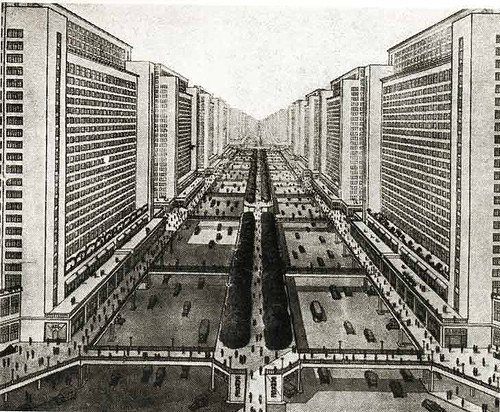
\includegraphics[width=10cm]{Illustrations/ville_radieuse.jpg}
\caption [The Radiant City, LeCorbusier (1924)] {LeCorbusier's large scale vision of a \textit{Radiant City} \index{Radiant City (1924)} introduced in 1924 suggested high density housing in form of monumental building blocks as a radical concept for a new quality of life. Large scale and repetitive architectural form refused to acknowledge the human scale and the characteristics of a vibrant public space.}
\label{RadiantCity}
\end{figure}

%%%%%%%%%%%%%%%%%%%%%%%%%%%%%

%\begin{singlespace}
%	\leftskip2.3em
%		\rightskip\leftskip
%			\textit{\small In her seminal book The Public Realm: Exploring the City’s Quintessential Social Territory, sociologist Lyn H. Lofland defines the public realm as that social entity within the physical settings of a city that is made up of interactions between  strangers—a successful public realm enables human interaction to take place. 
%} 	
%\end{singlespace}

%%%%%%%%%%%%%%%%%%%%%%%%%%%%%
 
Jane Jacobs \index{Jane Jacobs (1916-2006)} has been one of the early theorists who aimed to understand what constitutes public urban spaces.
Her book, \textit{The Death and Life of Great American Cities} (Jacobs 1961), is full of criticism on the then predominant post war urban planning, urban renewal and architecture. 
Rather than advocating for a particular architectural style Jacobs instead took a close look at the social behaviour of citizens in their local neighbourhoods. 
Jacobs' methodology was to conduct careful observations and conversations with residents in local neighbourhoods. 
She came to the conclusion that streets are the very essence of the city. 
Jacobs observed that the replacement of existing sound urban areas through up-scaling the built environment with residential super blocks, skyscrapers, shopping centres, monumental cultural centres and motorways, in other words the separation of function as proposed by Le Corbusier, led to the decline of former habitable areas, a lack of safety and the increase of poverty (Jacobs, 1961: 23-33).

Then in the 1970s \textit{The Street Life Project} \index{The Street Life Project (1980)} under the leadership of William H. Whyte \index{William H. Whyte (1917-1999)} systematically studied crowding on the streets of New York (Fig. \ref{fig:Whyte}). His research was driven by the question why some public spaces are more popular amongst dwellers than others. The observed imbalance of use in public space suggested practical implications \smalltodo[size=\footnotesize]{What are the practical implications? Could go in the appendix?.} towards a more liveable urban environment\cite{Whyte_1980} \footnote{In addition to the published book about the work conducted by \textit{The Street Live Project} a documentary has been released that clearly demonstrates the applied observations methods: \url{https://vimeo.com/111488563} [accessed 25.07.2016]}.


A comprehensive collection of attributes that describes what makes a great place originates from the non-profit-organisation \textit{Project for Public Spaces} \footnote{\url{http://www.pps.org/} [accessed 08.12.2016]} \index{Project for Public Spaces, New York} initiative in New York (Fig. \ref{great_place}). 
Eventually the sum of the successful implemented key attributes creates a specific identity of a particular place. \hyperref[placemaking]{}  

%%%%%%%%%%%%%%%%%%%%%%%%%%%%%
\begin{figure}[h] 
\centering
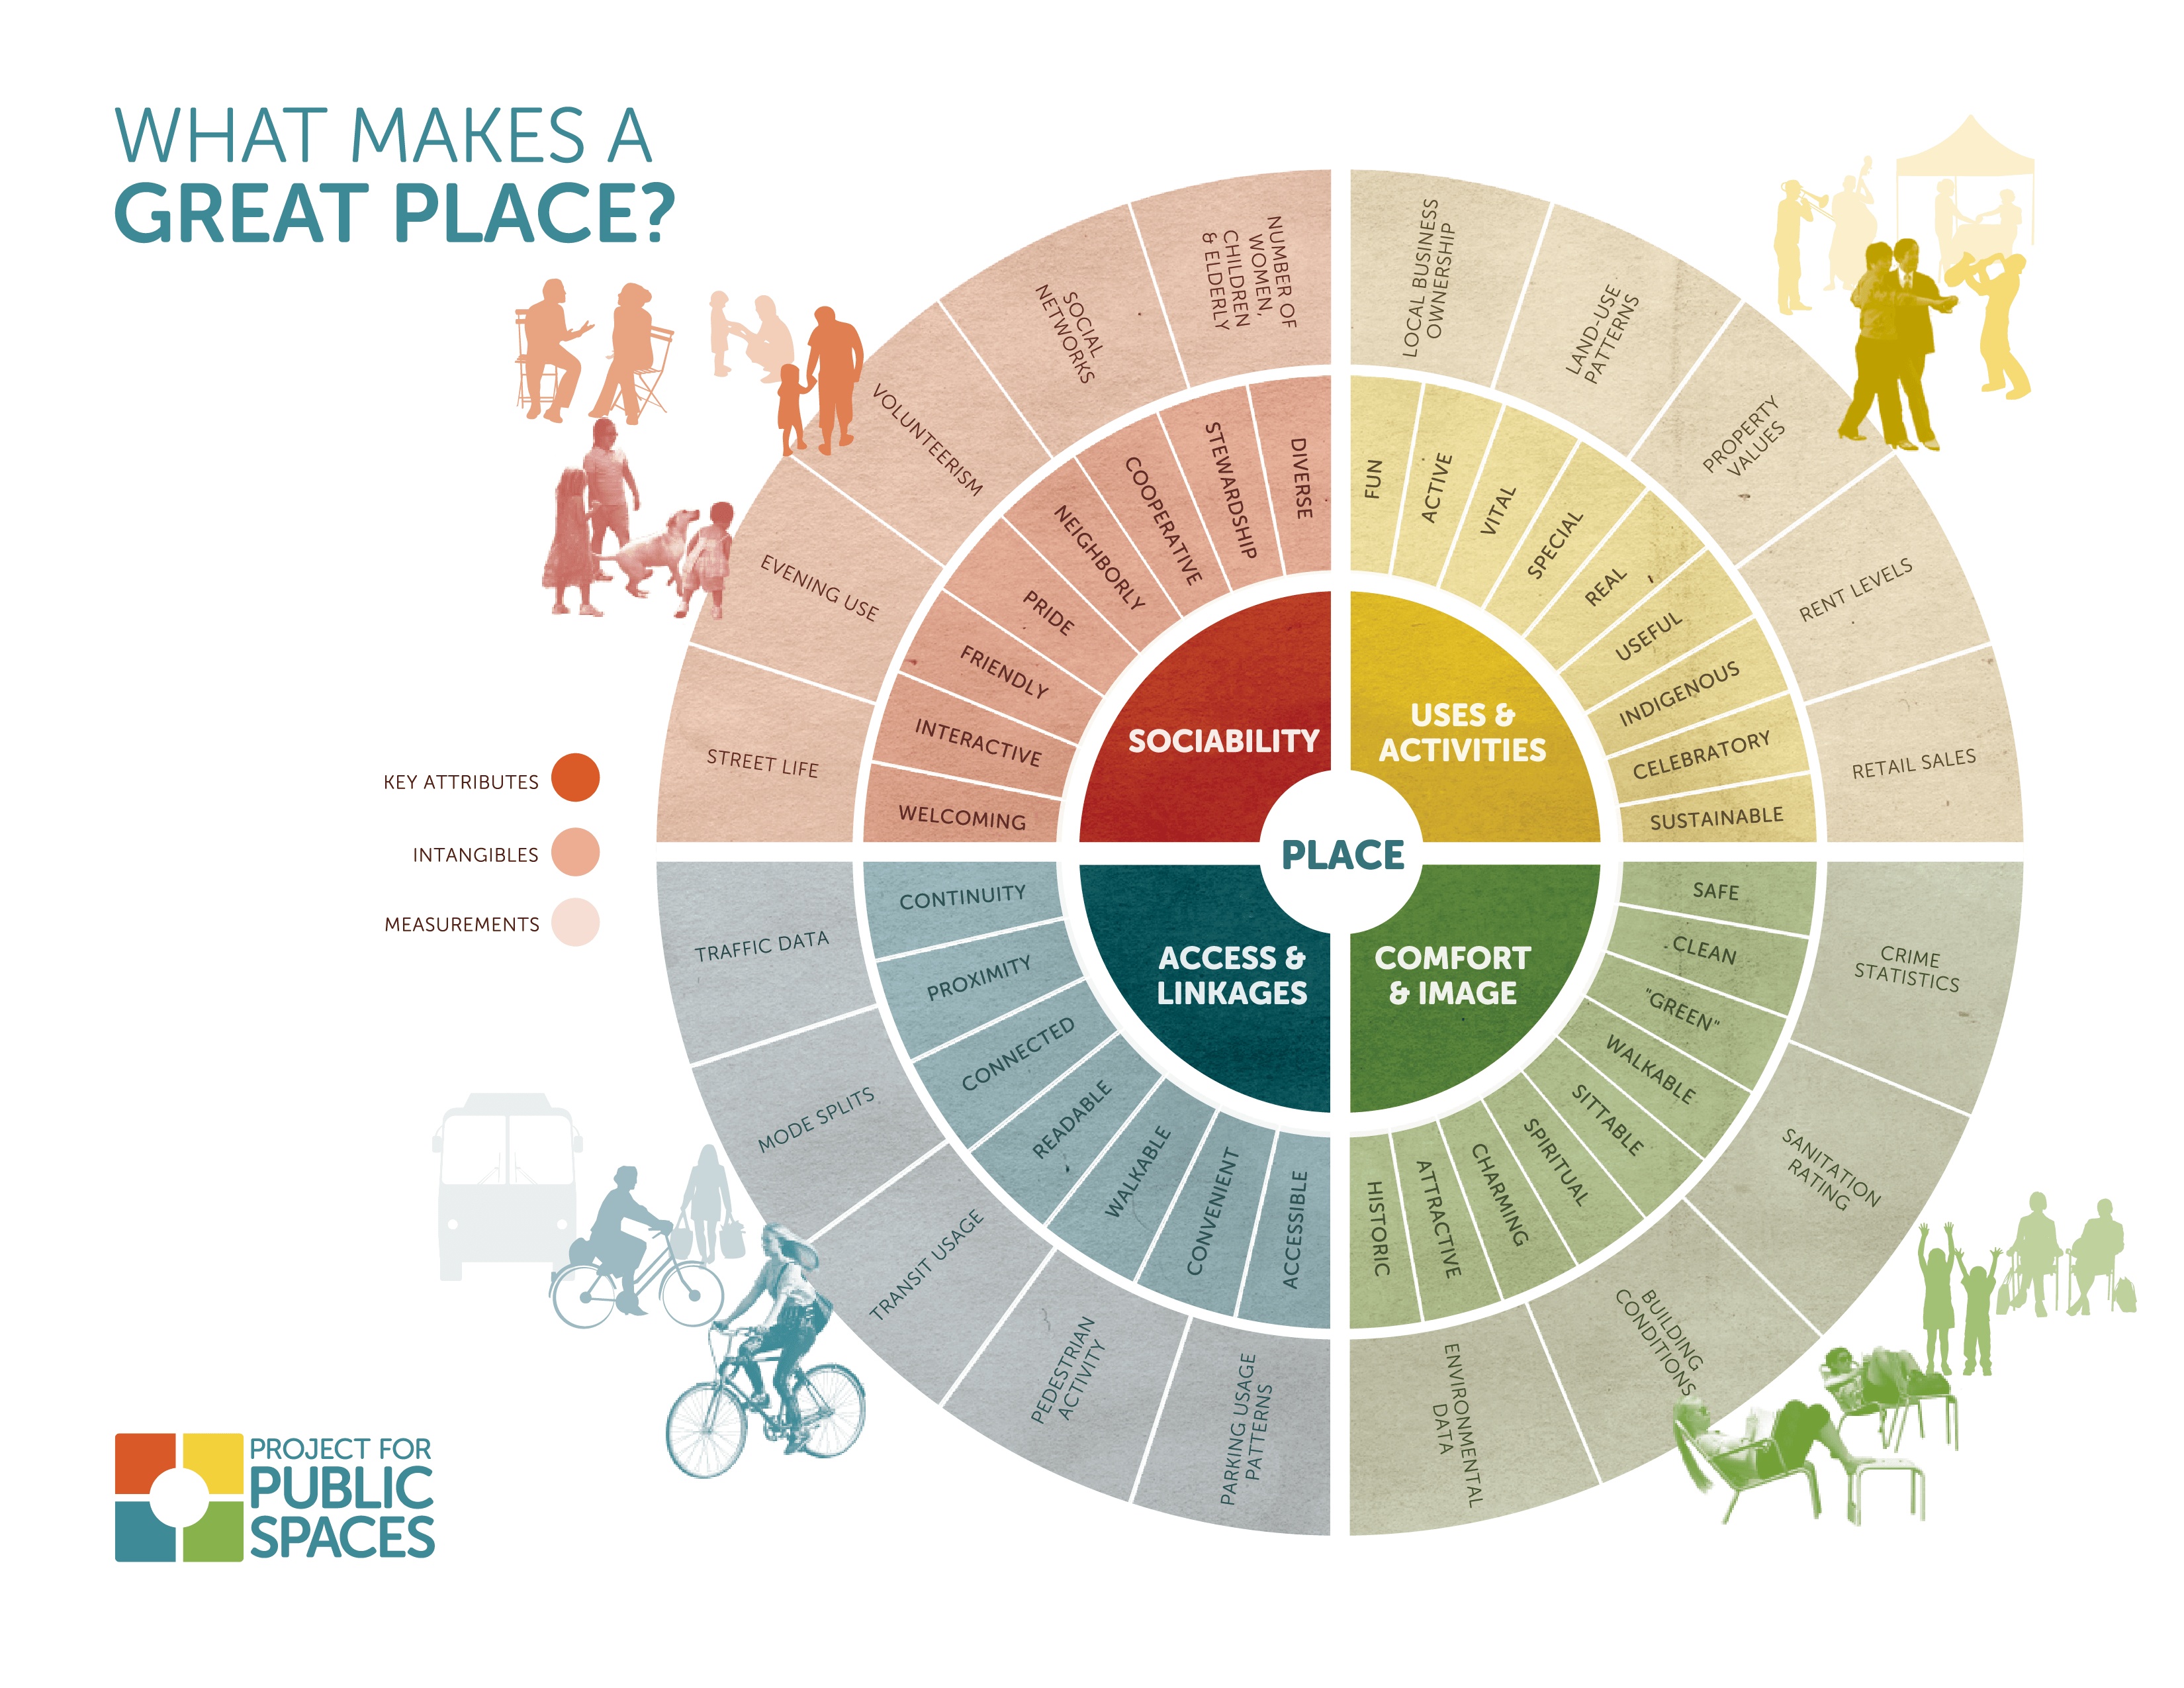
\includegraphics[width=10cm]{Illustrations/great_place.png}
\caption [What makes a great place?] {The four key attributes in the centre are surrounded by the intangibles and the indicator through which one can measure quality of the key attributes.}
\label{great_place}
\end{figure}
%%%%%%%%%%%%%%%%%%%%%%%%%%%%%

Around the same time in architectural research Bill Hillier developed his theory of what he called \textit{Space Syntax}. He generalised that cities need to be considered as an arrangement of architectural layouts that are defined through their relationships between physical space and social life reflected in movement patterns and activities of its inhabitants \cite{Hillier_1989}. 
To put it differently, \textit{Space Syntax} \index{Space Syntax} aims to analyse the spatial morphology of cities through researching the "relation of space to society, [which] is mediated by spatial configuration. Spatial configuration proposes a theory in which we find pattern effects from space to people and from people to space" \cite{Hillier1998}. This architectural theory as been applied and proofed in the fields of urban design (reference), architecture (reference), but also in cognitive science (Dalton et al., 2006) and in design and development of pervasive systems (Kostakos et al., 2009) and in particular in public displays (Dalton et al. 2010). In the meanwhile a methodological tool-set provided by Space Syntax facilitates the systematic study through spatial analysis and empirical observations of human behaviour such as pedestrian movement or social encounter in the urban realm \cite{AlSayed2013}.

%Dalton, R. C., Hölscher, C., & Turner, A. (2006). Space syntax and spatial cognition. Space Syntax and Spatial Cognition, (September), 1–201. https://doi.org/10.1177/0013916502238864
%Kostakos, V. (2009). Space Syntax and Pervasive Systems.
%Dalton, S. N., Marshall, P., & Dalton, R. C. (2010). Measuring environments for public displays. Proceedings of the 28th of the International Conference Extended Abstracts on Human Factors in Computing Systems - CHI EA ’10, 3841. https://doi.org/10.1145/1753846.1754066

The theoretical foundation of this research includes the description of the triangular relationship between a given Spatial Layout, the Attractor and Movement (fig. 2).
%Hillier, B. et al., 1993. Natural Movement: or, configuration and attraction in urban pedestrian movement. Environ Plann B. Available at: http://eprints.ucl.ac.uk/1398 [Accessed December 1, 2013].

%%%%%%%%%%%%%%%%%%%%%%%%%%%%%%%%

\begin{figure}[h!] 
\centering
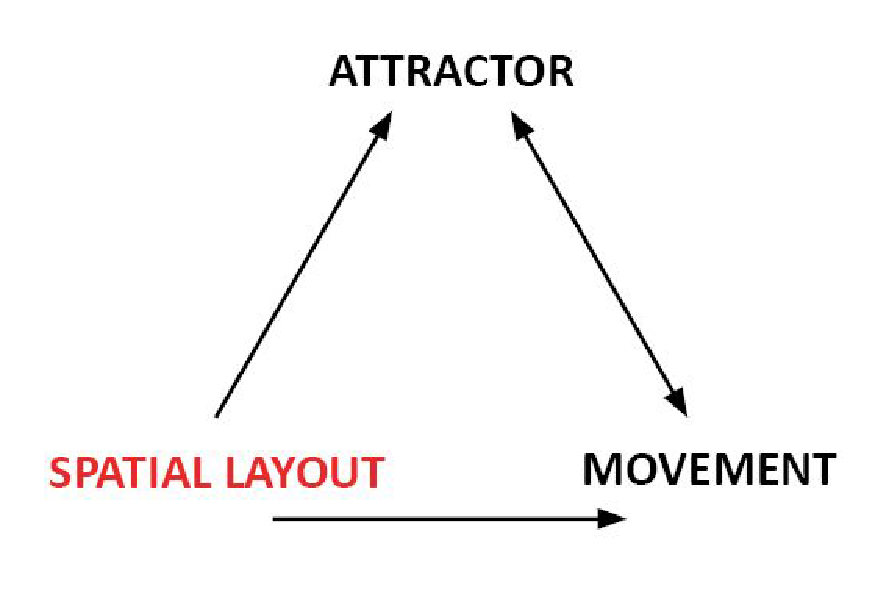
\includegraphics[width=6cm]{Illustrations/attractor_movement.pdf}
\caption [Spatial Layout, Attractor, Movement] {Socio-spatial configuration of public space: spatial layout, attractor and movement according to Hillier et al. (1993).}
\label{attractor_movement}
\end{figure}
\smalltodo[size=\footnotesize]{3D line drawing of an urban situation where the Spatial Layout has red lines, the attractor (i.e. a media facade) is blue and people within are marked green to illustrate the abstract sketch.}

%%%%%%%%%%%%%%%%%%%%%%%%%%%%%%%%

The arrangement of solid building blocks and the void space around it form the Spatial Layout \index{Spatial Layout}. Spatial layouts differ in their function and usage. Hence a central pedestrianised square differs from a traffic congested linear high street. 
Various Patterns of spatial layouts have been studied by Alexander (reference) and Lynch (reference).

\textit{Attractors}\index{Attractors} are physical objects which can be of different scale arranged  within the Spatial Layout that draw people's attention or entice people to step out of their daily routine. On a small scale attractors can be street furniture such as benches, ping-pong tables or water fountains, on a medium scale one can mention cafes, restaurants, bars and shops, whereas on a larger scale it could be historical facades, architectural landmarks or media facades. In this dissertation I consider large electronic surfaces such as urban screens or media facades as attractors. Besides their physical and spatial properties attractors have temporal qualities as well. For instance during rain one might avoid sitting on an outdoor bench and prefers to sit in a cosy bar, whereas during a warm summer afternoon people choose to enjoy cold beverages whilst sitting in front of a bar watching other people's activities.

Movement\index{Movement} is a major component in the formation of public space.
Seamon defines movement as "any spatial displacement of the body or bodily parts initiated by the person himself or herself" (Seamon, p.53). 
He further argues that the body and its extension in space and time are the essential components for an experience. Out of a sequence of movements and gestures evolves the ‘body ballet’ (Seamon, p.54). 
As soon as we locate the ‘body ballet’ into a specific physical environment we create the ‘place ballet’.
The type of movement - i.e. standing, strolling, rushing, running
Movement also has to do with people's attitudes. For example they rush to work in the morning whereas in the evenings they wander aimless through the city getting excited by different attractors.
The type of spatial layout and attractors within impact our movement. Transit spaces where people rush in order to catch a bus are different to public parks where people gather for pick-nicks.



A visible example of the triangular relationship described above is given by Jacobs:
Liveable streets in small scale neighbourhoods are the places where people meet and where commercial activities animated by cafes, restaurants, bars, bakeries and book stores take place. 
People love watching activities on the side walk generated by ordinary people, who run their daily errands (Jacobs). 
Jacobs wrote about primary children, who “dribble” to school, business men and elegant women heading for public transport and women in house dresses “criss-crossing with one another” and stopping for short conversations (Jacobs, 1961: 66-67). Jacobs identified this order of movements as a sidewalk ballet.
Not in a strict definition as a sequence of steps and movements in dance following a written notation but rather in a random alignment of improvisation of movements with ongoing new situations which demand human interactions (Jacobs, 1961: 65). 
At the same time one has to understand that the social activities in a public space change during the course of a day and even throughout the year.   
This is a glimpse on the strong spatio-temporal relation urban street life comprises. 


%‘Embodied interaction’ (Dourish, 2001), which describes action of the 'body' or user interacting with embedded technology (and thus potentially linking to social networks) is another important component in location-based applications

The given Spatial Layout, Movement and Attractors are interdependent key properties of what I will call in this dissertation \textit{socio-spatial configurations}. It is to notice that a given Spatial Layout may impact the configuration of Attractors and Movement. Attractors and Movement do influence each other, whereas neither of the both have an impact on the Spatial Layout 


\paragraph{The Digital Shift}

At the same time the city undergone a radical shift widely invisible and hidden from most citizens. The 'invisble city' (Lewis Mumford) 


In the meanwhile: 

%%%%%%%%%%%%%%%%%%%%%%%%%%%%%%%%

\begin{singlespace}
	\leftskip2.3em
		\rightskip\leftskip
			\textit{\small The visible city as a prime determinant of the urban is an artifact of the past. Instead, it is what Lewis Mumford called the "invisible city," the world of cables, wires, connections, codes, agreements, and capital that increasingly dominates our networked society [Lewis Mumford]. We stand at the dawn of the regime of the invisible, its role in determining urban structure vast. The visible becomes an irruption of other forces, a graphic user interface for a more powerful command line below [Varnelis].}
\end{singlespace}

%%%%%%%%%%%%%%%%%%%%%%%%%%%%%%%%

Based on Mamford Kittler concluded that the City as a Medium (Kittler, 1996)
 
%Thus she set up four conditions to improve street life. 
%First, she claims for street activities at all hours of the day. 
%Neighbourhoods have to attract all kinds of different people. 
%This is attainable through a mixture of uses and functions, both socially and economically. (Jacobs, 1961: 198-232) 
%Her second condition is the building of short blocks and intricate street structures which provides the possibility for pedestrians to explore different walks (Jacobs, 1961: 233-243). 
%Variation of buildings in age and function is the third condition for successful street life (Jacobs, 1961: 244-260). 
%The last one is density, because the higher the concentration of people in one place is the more attractive the area. 
%Neighbourhoods with working vivid street life determine safety, social cohesion and economic growth is Jacobs' conclusion (Jacobs, 1961: 261-289).
%To summarize, one can say that Jacobs' criticism of the prevailing architectural styles and urban planning ideologies and her persistent observations on \textit{life in between buildings} (book title by Jan Gehl) initiated a shift from form-follows-function towards a behavioural centric age.  

%With the advent of the digital our built environment has turned into an ecology of sensors measuring our behaviour in public. Human-computer interfaces such as mobile devices, urban screens or media facades augment our physical presence in digital space. 

%%%%%%%%%%%%%%%%%%%%%%%%%%%%%
In summary: Whilst modernist architects (references) focused on the physical properties of humans Jacobs and others (Seamon, Goffman, ...) explored human behaviour in relation to public space. 
Jan Gehl later accused this architectural period of lacking the people scale, which needs to work on eye-level and 5km/h perception, which in a nutshell was the method Jacobs applied in her observations. Whilst architects persistently neglected the importance of public spaces for creating social interactions Jan Gehl was one of the pioneers who put the results of his research into practice \cite{Gehl_2013}. 

To summarise 
I briefly summarised the notion of public space .
In this section I defined what I consider spatial configuration, namely the triangular relationship between Spatial Layout, Movement and Attractors. 
what I consider the notion of public space with regards to this research is: 
Firstly public space is constituted through the three components of Spatial Layout, Movement and Attractors. 
Guidelines on how to approach public spaces when designing for interactions include:
The people scale as suggested by Gehl.
Some of the conditions Jacobs suggested:
Street activities need to take place during all hours of the day. I would argue that this increasingly includes the hours of night. Further a mixture of uses and functions, both socially and economically. 
Designing for density, the more people there are in one place the more attractive this area is - of course overcrowding leads to the opposite. 

In the next section I will investigate what interactions are and how technology may assist in mediating those interactions in public space.


%%%%%%%%%%%%%%%%%%%%%%%%%%%%%

\section{Shared Encounters and Technology Mediated Interactions in Public Spaces}

Only recently digital technologies entered the public domain in form of mobile devices or large situated electronic surfaces and discussions are ongoing whether digital technologies affect social interactions in public space have adverse effects \cite{Turkle_2012}, have no impact \cite{Hampton_2015} or can be seen as an opportunity to create mediated participatory experiences \cite{Gordon_2011}. Hence the key concept of \textit{Public Space} and the triangular relationship between Spatial Layout, Attractor and Movement is followed by a review of research into what constitutes a shared encounter and how it differs from an interaction in public space.

Encounters are different in their nature and are situated either in private or in public spaces. They are individual or grouped and either they are planned or happen by chance. The characteristics of shared encounters have been characterised by Willis et al. (2010) as:

%%%%%%%%%%%%%%%%%%%%%%%%%%%%%%%%%

\begin{singlespace}
	\leftskip2.3em
		\rightskip\leftskip
\textit{\small the interaction between two people or within a group where a sense of performative co-presence is experienced and which is characterised by a mutual recognition of spatial or social proximity} 

\small Taken from  Willis et al. (2010) p.4
\end{singlespace}

%%%%%%%%%%%%%%%%%%%%%%%%%%%%%%%%%
Today, as ICTs are ubiquitous and mobile, people interacting with each other does not require them to be in the same physical space any more, instead we create co-presence where two people interact with each other without being in the same physically space. Hence the encounter is technology mediated and therefore defined as a shared encounter.
Social spaces are defined as a series of interactions and their nature is volatile - movement.

%Willis: "our interactions with other can be considered as situated in that they are shaped by both the physical setting and the social situation - consequently we behave differently in different situations"
%Willis: "Social spaces emerge through multiple one-to-one interactions and by participation in groups. These encounter spaces can disperse as rapidly as they are created, but some can become more established and exist for a period of time."
Goffman (reference) describes the part performance plays in an interaction; performances are a set of activities of an individual before a set of observers - either friends of strangers

Social encounters are defined as unplanned ad-hoc gatherings amongst (un-) known people. Research has defined ‘shared encounters’ as mostly context aware. The physical setting in which an encounter takes place is relevant (Goffman, 1963), hence the "built environment creates stages for shared encounters but sometimes the features of built space can actually hinder rather that allow these shared experiences" (Garcia). Therefore the type of encounter stage and its information context impacts the kind of shared encounters. Encounter stages are public spaces “on which people negotiate boundaries of a social and cultural nature” (Fatah et al, 2005). For example at bus stops social chance encounter happen when people ask for directions or start conversations about the delayed schedule. One objective of this research will focus on the particular spatial properties physical encounter stages require in order to support shared encounters.
\smalltodo[size=\footnotesize]{This argument can be confirmed in my findings of the case studies - e.g. participants in Sao Paulo and Linz were discussing the impact of public visualisations. }

 

(Willis, Shared encounters)).
Fatah defines three different types of encounters Fig. \ref{DigitalEncounterFatah}). 
and consequently a "concept of a digital stage that can facilitate and encourage different types of social encounters" has been developed. 

%%%%%%%%%%%%%%%%%%%%%%%%%%%%%

\begin{figure}[h!] 
\centering
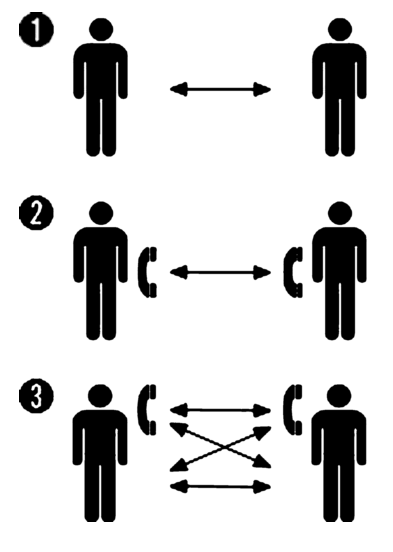
\includegraphics[width=3cm]{Illustrations/DigitalEncounterFatah.png}
\caption [Digital Encounter Fatah] {Digital Encounters: Human communication (1), communication replaced by technology (2), or augmented by technology (3).}
\label{DigitalEncounterFatah}
\end{figure}

%%%%%%%%%%%%%%%%%%%%%%%%%%%%%

To summaries: 

- need to build in ‘familiar stranger’ (Milgram 1977)

\subsection{Urban Interaction Design - Urban IxD}

%%%%%%%%%%%%%%%%%%%%%%%%%%%%%

Interaction Design (IxD) is a relatively new discipline that merges design with digital technologies and behavioural science and hence founded on divers academic and applied fields (Fig. \ref{DesignFields}).
IxD is about creating interactive products for the user experience to "enhance and augment the way people work, communicate and interact" (\cite{Rogers_2015} p.9).
Research into Human-Computer Interaction (HCI) has spawned Interaction Design \cite{Rogers_2015} to better understand "wicked problems" (Rittle and Webber, 1973; Fitzgerald, 2003; Zimmermann, 2007) created through sometimes unpredictable human behaviour.
%Rittel, H.W.J. & Webber, M.M., 1973. Dilemmas in a general theory of planning. Policy Sciences, 4(2), pp.155–169.

%%%%%%%%%%%%%%%%%%%%%%%%%%%%%

  \begin{figure}[h!]
  \centering
  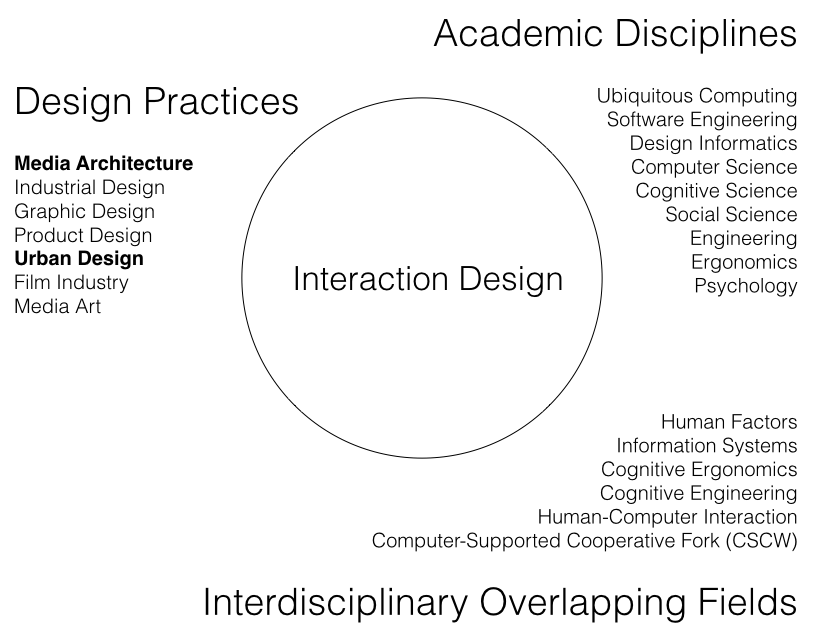
\includegraphics[width=8cm]{Illustrations/Interaction-Design-Fields.png}
  \caption{What is Interaction Design? \cite{Rogers Interaction Design - beyond HCI 4th Edition p. 9} - What is missing here is the overlapping of interaction design and media architecture.}
  \label{DesignFields}
  \end{figure}

%%%%%%%%%%%%%%%%%%%%%%%%%%%%%
The invention of the computer mouse by Engelbart in 1963 might be seen as the first IxD product as it incorporates knowledge from design, behavioural science and computer technologies.   
Apple's iPod in turb can be considered as one of the first commercial IxD products with global success that follows clear IxDs principles (Moggridge, 2006). Here the touch interface and the required gestures to use the portable music player is pioneering IxD. 
%Moggridge, B., 2006. Designing interactions - Chapter 1, Available at: http://site.ebrary.com/lib/aalborguniv/reader.action?docID=10173639.

IxD mostly develops screen-based applications and services for desktop computers or more recently for mobile devices such as smart phones or tablets. However, since the advent of ubiquitous computing (Weiser, 1991), and its application in urban space in the form of urban computing (Kindberg et al., 2007), the built environment incorporates architecture and ubiquitous computing technologies. Consequently IxD entered the urban domain and began to design way finding or location based applications that let user experience services such as bike or car sharing in new ways.
%The Internet of Things (IoT) is another application worth mentioning in this context.

In academia the research project "Digital Urban Living" at the Aarhus University was the first larger attempt to explore IxD in an urban context \footnote{http://digitalurbanliving.projects.cavi.au.dk/ accessed 29.11.2016} Within this project researchers and designers in collaboration with the CAVI centre \footnote{http://cavi.au.dk/about-cavi/ accessed 29.11.2016} implemented amongst others "Aarhus by Light" \footnote{http://cavi.au.dk/research-areas/aarhus-by-light/ accessed 29.11.2016} media facade project at the Concert Hall in Aarhus (Brynskov et al., 2009) that explored interactive systems for user engagement in urban space.
%Brynskov, M. et al., 2009. Staging urban interactions with media facades. In Lecture Notes in Computer Science (including subseries Lecture Notes in Artificial Intelligence and Lecture Notes in Bioinformatics). pp. 154–167.

%%%%%%%%%%%%%%%%%%%%%%%%%%%%%%%
\begin{figure}[h!]
  \centering
  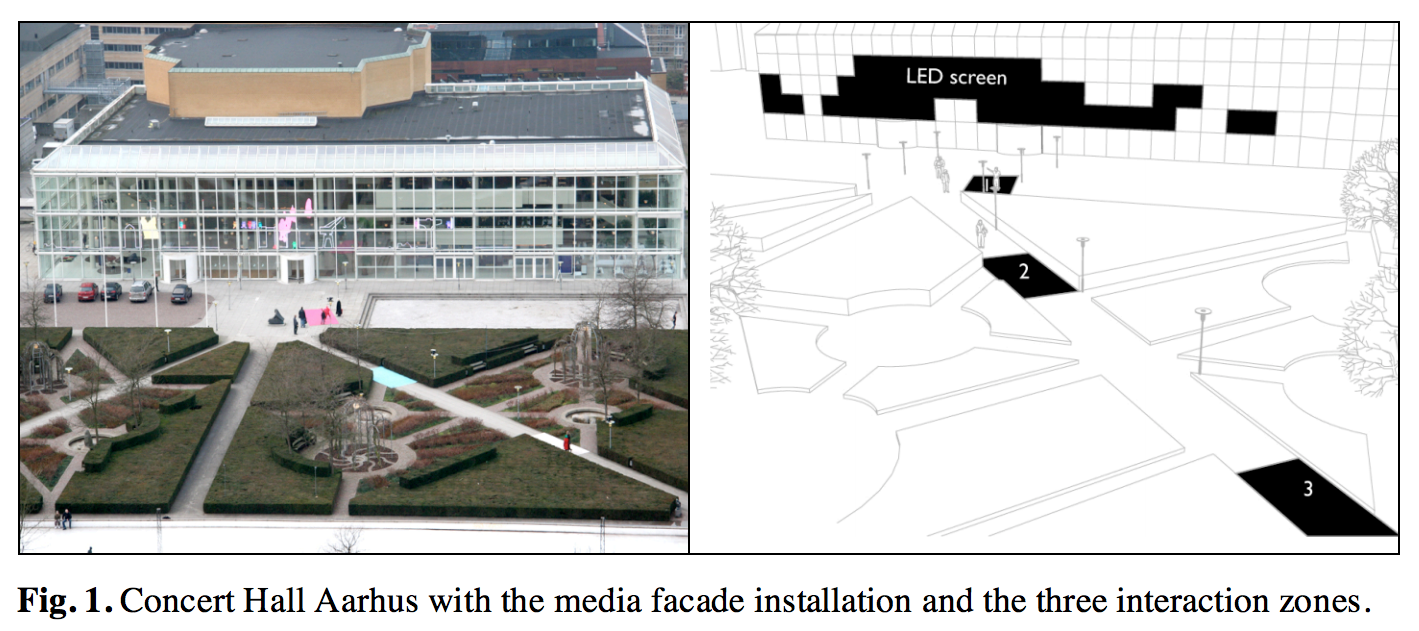
\includegraphics[width=14cm]{Illustrations/AarhusbyLight.png}
  \caption{Aarhus by Light}
  \label{AarhusbyLight}
  \end{figure}
%%%%%%%%%%%%%%%%%%%%%%%%%%%%%%%

From the spatial perspective (which will be discussed in detail later in this backround research) urban IxD benefited from Fischer's and Hornecker's research into an understanding of interaction spaces in public spaces \cite{Fischer_2012}.
Whilst designing for interactions mediated by interactive technology in public spaces has been predominately occupied by HCI and IxD there are academic initiatives and projects from architectural research and practice (Behrens, 2013).
%Behrens, M. (2013). Exploring the effect of spatial layout on mediated urban interactions. Proceedings of the 2nd …. Retrieved from http://dl.acm.org/citation.cfm?id=2491586

- Screens in the Wild
- 


Early social implications of interactive systems on urban grassroots movements have been explored by the HCI community during a CHI \footnote{ACM Conference on Human Factors in Computing Systems (CHI)} workshop in 2011 by (Kuznetsov et al., 2011).
%Kuznetsov, S., Odom, W., Paulos, E., Disalvo, C., Moulder, V., Wakkary, R., & Hirsch, T. (2011). HCI , Politics and the City : Engaging with Urban Grassroots Movements for Reflection and Action. Design, 2409–2412. http://doi.org/10.1145/1979742.1979568

The social aspects in urban IxD are currently explored in the European wide network called OrganiCity. The approach is to provide "cooperation and participation, for collaborative city experiments developed with, and at the initiative of, citizen groups, organisations, authorities and companies." In several projects across European cities the advancement of participatory city making mediated by digital technologies and IxD are investigated.  \footnote{The EU funded OrganiCity initiative connects leading smart cities Aarhus, London and Santander with the aim to "put people at the centre of the development of future cities." http://organicity.eu/ accessed 25.11.2016}

Urban IxD and wellbeing have been explored by  

%usability goals for a sustainable user experience which are: the effectiveness of use (how good is a product at performing as it should do?), the efficiency of use (Is the device able to sustain a high level of productivity?), the safety of use, the utility (Does the product provide an appropriate set of functions that will enable users to carry out their tasks in the way they want to do them?), the ease of learning (Is it possible to work out how to use the product by exploring the interface and trying out certain actions?) and the memorability of usability (What kind of interface support has been provided to help users remember how to carry out tasks?).

Research into IxD has brought forward several frameworks for designing interactions in urban space.
- technical aspects
-social aspects
- spatial aspects Daalsgarqd, Halskov ... 
From behavioural perspective designing for interactive products the following principles have been established by : "1) Affordance: This term refers to the question How easy is it to find out how to use it?. Thus a physical object has to explain itself in relation to how to use it by its obvious perceptional appearance. (Norman, 1988). 
2)Visibility: Controlling devices such as buttons basically have a very clear visibility. But far more important is the positioning of a device in the environment. If people cannot find the device, there will be no interaction (Rogers, 2011).
3) Accessibility: An interactive device has to be accessible by as many people as possible. Especially nowadays where technical progress is accelerating the integration of as many groups of people as possible this is an important aspect in interaction design. (Rogers, 2011; Negroponte, 1995)
and finally 4) Feedback: An immediate feedback such a flashing light or audio signal by the device is a crucial element to let the user know that the interaction works (Rogers, 2011)."	



These requirements are therefore integral part of the development of our project. 

%In the context of interaction design around public displays in an urban context the following research projects can be aligned:
%Elmar Trefz and Joanne Jakovich: Rapid Probing: Setting out methods and a framework for Urban Interaction Design - Media City 4
%- Urban IxD projects in research:
%1. Community notice board Sydney
%2. MyPosition
%3. Lisa Koeman, V Kalnikaite, Yvonne Rogers, Jon Bird	What chalk and tape can tell us: Lessons learnt for next generation urban displays	2014	PerDis 2014 - Proceedings: 3rd ACM International Symposium on Pervasive Displays 2014, Journal article

In summary: Designing means knowing your limitations and constraints. This is a finding that applies to architectural designing and IxD designing for interactions. 
This thinking applies for research as well.

%%%%%%%%%%%%%%%%%%%%%%%%%%%%%%%

\begin{singlespace}
	\leftskip2.3em
		\rightskip\leftskip
\textit{\small Good design comes from the successful synthesis of a solution that recognises all the relevant constraints, and the nature of the constraints defines the difference between the design disciplines.} 

\small Taken from Moggridge (2006) p.649.
\end{singlespace}

%%%%%%%%%%%%%%%%%%%%%%%%%%%%%%%

\subsection {City as Interface}

For some people to be able to encounter new people or to interact with each other without being in the same physical space interfaces that mediate communication may assist.
Today such interfaces are ubiquitous, we seem to have established an "interface culture" (Johnson, 1997) 
%Interface Culture: How New Technology Transforms the Way We Create and Communicate)
in which individual mobile devices or shared and situated large electronic surfaces structure our everyday lives (Saggio,).
However definitions of what interfaces in public spaces actually constitute are blurry and due to their interdisciplinary usage manifold.  

Going back to the early considerations in computer science, Yershov suggested the properties needed for a "dialogue between man and machine" (Yershov,). In his understanding an interface has to be "conform to the characteristics of interpersonal communication, since these are rooted in the characteristics of human intelligence."
Nevertheless the user needs to train himself to be able to communicate with the machine. 
This finding complements the notion of digital encounters as described in the previous section.
Interpersonal communication has been studied by Norman (1988).
%Norman, D. (1988) The Design of Everyday Things.
%Goffman, E.: Behaviour in Public Places. The Free Press, New York (1966)
%There is even a whole new profession of so called interface designers.

%%%%%%%%%%%%%%%%%%%%%%%%%%%%%%%

\begin{figure}[h!] 
\centering
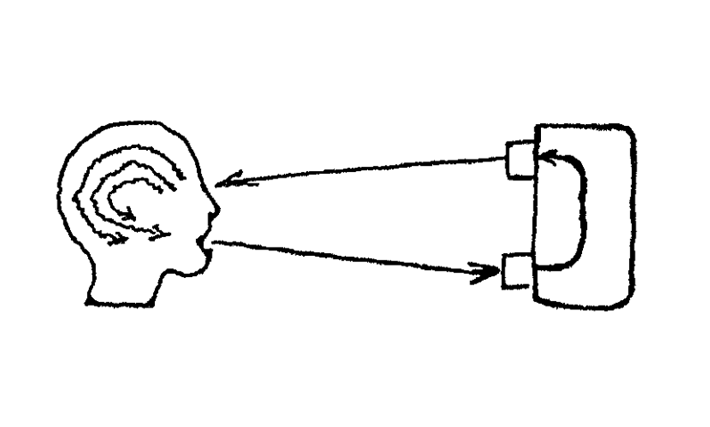
\includegraphics[width=8cm]{Illustrations/Yershov.png}
\caption [Director-agent interaction diagram by Yershov (1965)] {"The machine above all as a means of automating the mental activities of man, or as - this term seems more appropriate - an amplifier of the mental abilities of man" (Yershov, 1965). Negroponte (1970) commented, that the three arrows within the human brain compared to the single arrow within the machine would imply "an ever-continuing act particular to the role or constitution of the man and not the machine."}
%“The Architecture Machine” by Nicholas Negroponte (published by the MIT in 1970). 
\label{Yershov}
\end{figure}

%%%%%%%%%%%%%%%%%%%%%%%%%%%%%%%
These early considerations of how humans interface computers has led to the research domain called human-computer interaction.
One is aware of the early interfaces that emerged during the what is called "2nd wave" of HCI, when Tangible User Interfaces (TUIs) such as the mouse and keyboard together with Graphical User Interface (GUI) gave access to yet bulky computers. 

While it has been claimed that so called Graphical User Interfaces (GUI) are the most widely spread products of HCI that allow humans to interface with computers,  Tangible user interfaces (TUIs) "give physical form to digital information, employing physical artifacts both as representations and controls for computational media" \cite{Ullmer_2000}(p. 916). 
\textit{Tangible Interactions} evolved from research in TUI and rely on embodied interaction, tangible manipulation, physical representation of data and embeddedness in real space and give computational resources and data material form \cite{Hornecker_2006}. 

Others argue that the shift from situated (i.e desktop computer) to mobile interface (i.e. mobile phones or tablets) and its ubiquitous use in public space blurs the boundaries between the physical and the digital social networks and hence interfaces can be described as 'social interfaces'(de Souza e Silva, 2006).  

%%%%%%%%%%%%%%%%%%%%%%%%%%

\begin{singlespace}
	\leftskip2.3em
		\rightskip\leftskip
\textit{\small I propose a further conceptualization of “social interface,” which defines a digital device that intermediates relationships between two or more users. Within this context, social interfaces not only reshape communication relationships but also reshape the space in which this interaction takes place.} 

\small Taken from de Souza e Silva, A. (2007) p.261-262
\end{singlespace}

%%%%%%%%%%%%%%%%%%%%%%%%%%
%de Souza e Silva, A. (2007). From cyber to hybrid: Mobile technologies as interfaces of hybrid spaces. In D. Bell & B. Kennedy (Eds.). The Cybercultures Reader 2.0 (pp. 757-772). London, New York: Routledge. (re-print from Space and Culture journal).
And beyond the social component de Souza e Silva refers to the impact social interfaces ultimately have on the space in which they take place. This is in line with the notion of encounter stages. 

Hookway understands interfaces as a "relation with technology" rather than a technology in itself (Hookway, 2014).

%%%%%%%%%%%%%%%%%%%%%%%%%%

\begin{singlespace}
	\leftskip2.3em
		\rightskip\leftskip
\textit{\small The interface is a form of relation that obtains between two or more distinct entities, conditions, or states such that it only comes into being as these distinct entities enter into an active relation with one another; such that it actively maintains, polices, and draws on the separation that renders these entities as distinct at the same time as it selectively allows a transmission or communication of force or information from one entity to the other; and such that its overall activity brings about the production of a unified condition or system that is mutually defined through the regulated and specified interrelations of these distinct entities.} 

\small Taken from Hookway, B., 2014. Interface, p. 4
\end{singlespace}

%%%%%%%%%%%%%%%%%%%%%%%%%%
And for Galloway "interfaces are not simply objects or boundary points. They are autonomous zones of activity. Interfaces are not things, but rather processes that effect a result of whatever kind."
According to Galloway's notion of Interfaces defines "Activity zones", which is in support of the idea of social encounter stages as defined by (ref.) 
Verhoeff (reference) finally summarises that: "Following Branden Hookway and Alexander Galloway, I understand media interfaces as processes rather than objects. An interface is not something; it does something."
%Urban Interfaces: The Cartographies of Screen-Based Installations by Nanna Verhoeff (2016)
%Due to technological advancement, large public displays became ever more incorporated into the built environment and because of price decline its application for social and artistic purposes became popular in urban space. 
%This led to novel technology-mediated social interactions, such as people engaging with media facades through tangible devices.


Seen from architectural research Martyn Dade-Robertson (2013) introduces Architectural User Interfaces (AUIs) taking into account Graphical User Interfaces (GUIs) and argues that architectural design and HCI can benefit immensely from each others.
Dade-Robertson refers to McCullough (2004) who back then saw:

\begin{singlespace}
	\leftskip2.3em
		\rightskip\leftskip
\textit{\small Digital networks are no longer separated from architecture. Unlike cyberspace, which was conceived as a tabula rasa, pervasive computing has to be inscribed into the social and envirnonmental complexity of the existing physical environment.} 

\small Taken from Malcom McCullough, 2004. Digital Ground, page 4.
\end{singlespace}

Dade-Robertson concludes that the future of architectural design is accompanied by cognitive science and situated and pervasive interfaces.
%McCullough, Malcom, 2004, Digital Ground: Architecture, Pervasive Computing and Environmental Knowing, MIT Press
%(Dade-Robertson, M. (2013). Architectural User Interfaces: Themes, Trends and Directions in the Evolution of Architectural Design and Human Computer Interaction. International J of Architectural Computing, 11(1), 1-19.)

Martijn de Waal even extends the notion of an interface and considers the whole city as an interface.

%de Waal, M., 2014. The City as Interface - How Digital Media are Changing the City.

One of the first large scale social media art projects that provided an interface allowing passers-by to create and share content on a media façade was the BlinkenLights \footnote{http://blinkenlights.net/blinkenlights accessed 28.11.2016} project in 2001. Participants on a street in Berlin were able to share messages typed into a mobile phone with the public through posting them on a low-resolution media facade (each pixel was represented through an illuminated window in an office building (i.e. Haus des Lehrers, Alexander Platz, Berlin)). 
Since then numerous media art and research projects have been developed and presented that include user interfaces and applications to transmit actions, in situ and in real-time, on to a media facade that is connected to an interface. 
For example, SMSlingshot \cite{Fischer_2012}, Sonic Skate Plaza \cite{Serret_2013} or Binoculars \cite{Guljajeva_2013}.
In applied HCI research, more recently, multi-user interactions with media facades through mobile devices revealed challenges when deploying interactive artifacts in urban space that enable passers-by to engage with media facades \cite{Boring2011}. 
Wiethoff and Gehring \cite{Wiethoff2012} introduced a design toolkit to prototype when designing interactions with media facades before the actual deployment. 
\index{In-the-air-tonight} A media facade project that explored mobile interfaces to rise awareness of social issues in Toronto has been developed by the Ryerson Image Centre. During winters night the LED facade is turned in blue to represent the wind speed, as soon as the hashtag \#homelessness appears on Twitter the building's facade flashes up in red light \footnote{http://www.intheairtonight.org/ accessed 28.11.2016}. 

Since then, novel interfaces have been designed and deployed in the urban environment that let people interact with media facades \cite{Hoggenmueller_2014}.

%Fischer, P.T.; Hornecker, E., 2017. Creating Shared Encounters Through Fixed and Movable Interfaces. , pp.163–185. Available at: http://link.springer.com/10.1007/978-981-10-1962-3.

In summary: HCI considers interfaces as pure physical or graphical representations that allow users to access computer technologies. Today different disciplines understand that interfaces unfold temporal, social, spatial and cultural dimensions and designing interfaces can not neglect these dimensions.
What does it mean when one aims to design for interactions with media architectures?



%%%%%%%%%%%%%%%%%%%%%%%%%%%%%

\subsection{Communication Technologies for Mediated Encounters}

WiFi
Bluetooth
RFID

%%%%%%%%%%%%%%%%%%%%%%%%%%%%%

\subsection{Public Display Research}

Long before research into public displays \index{public displays} became a domain within HCI, various kinds of electronic displays and digital signage appeared in public spaces.
At the New York Times building the first public display, \textit{The Motogram} \index{The Motogram (Zipper)} also called \textit{The Zipper}, was installed in 1928 (Fig.\ref{DigitalSignage} (left)). The novel display consisted of a band of light bulbs (dot matrix\footnote{two-dimensional array of programmable objects, in context of this dissertation the objects are light- bulbs or LEDs}) that circulate breaking news along the facade. 
Almost fifty years later, in 1976, the same building got upgraded with the first large programmable electronic surface called \textit{Spectacolor Board} \index{Spectacolor Board}(Fig.\ref{DigitalSignage} (right)).
The rather conventional rectangular screen was mounted to the slim front side of the corner building facing towards Times Square; unlike \textit{The Motogram's} slim horizontal luminous strip which ran across all sides of the publishing house visually separating the building in a lower and an upper part. 
From an architectural point of view the analogue light bulb display conforms the architecture of the building through adapting to the characteristics of the facade. Whereas the \textit{Spectacolor Board} appears to be an oversized TV screen - attached to a wall that is too little. However, the \textit{Spectacolor Board} provides more opportunities for content creation as well the direction it is facing towards (i.e. Times Square) is very likely to reach a larger audience. Whilst \textit{The Motogram} due to its elongated shape is limited in content and can hence only show continuous running text it is specifically designed for the news agency New York Times.
Consequently, I argue that \textit{The Motogram} can be considered to be architectural compared to the \textit{Spectacolor Board}, which constitutes a public display in the form of an Urban Screen instead.

%%%%%%%%%%%%%%%%%%%%%%

\begin{figure} [h!]
    \centering
        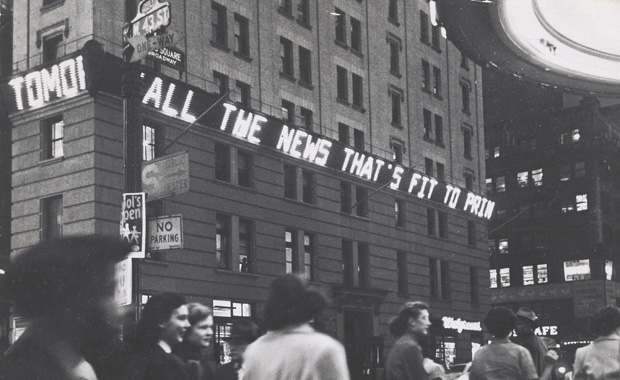
\includegraphics[height=4.5cm]{Illustrations/zipper.jpg}
        	%\caption[a]{Urban Screen}
      	%\label{UrbanScreen}
        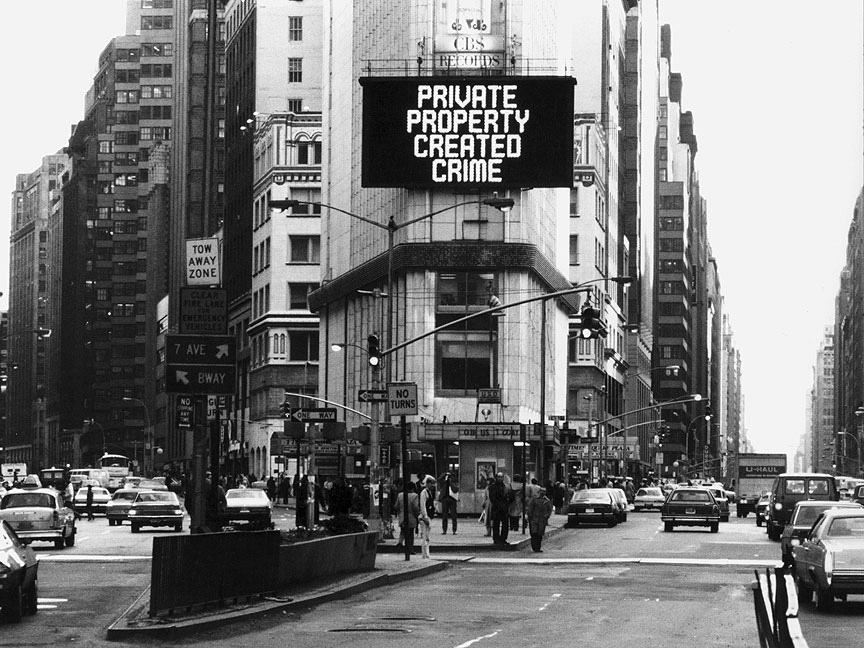
\includegraphics[height=4.5cm]{Illustrations/Spectacolor_JennyHolzer_.jpg}
       		%\caption[b]{Media Facade}
       	%\label{MediaFacade}
    \caption[First public displays]{Innovativ public displays at the New York Times Square: \textit{The Motogram/Zipper} display (left), and the \textit{Spectacolor Board} (right)}
    \label{DigitalSignage}
\end{figure}

%%%%%%%%%%%%%%%%%%%%%%

In the meanwhile public displays \index{public displays} are everywhere - mostly for commercial or informational purposes. Large screens at traffic junctions dazzle car drivers with dynamic advertising and at bus and train stations or airports huge displays update us on the latest travel news.  

Research in public displays \index{public displays} arose as observations by HCI researchers hinted towards different kind of human behaviour when having a home display in a public space for shared purposes. 
(Mention Rogers in the Wild?)
Although utility, usability and likeability seemed to be identical it has been obvious that different requirement such as "public displays need to grab the attention of passers-by, motivate passers-by to interact with them, and deal with the issues of interaction in the public" (Mueller et al., 2010) 
%(Müller, J. et al., 2010. Requirements and design space for interactive public displays. In Proceedings of the international conference on Multimedia. pp. 1285–1294.)
This relates back to Movement.

\textbf{Different Form Factors}
Whilst most public displays have conventional formats to easily be able to show cross platform content, the form factors of some displays vary and yet "it’s difficult to say whether display walls, windows, magic mirrors, or something completely different will become a dominant form for digital signs, but it’s likely that use of digital displays will continue to increase dramatically." (Want and Schilit, 2012). 
%Want, R. & Schilit, B.N., 2012. Interactive digital signage. Computer, 45(5), pp.21–24.

(Show figure of Florian Alt's shape shifting study of the public display at Munich Airport.)

\textbf{Interactivity}
In this context interactivity ar  ound those displays becomes ever more important. In the meanwhile the audience - in particular children - expect digital signage to in corporate touch features \footnote{This is an observation we frequently made during field observations in the Screens-in-the-Wild project.}. 



I will specifically refer to research in public display here as methods have been well advanced and many studies were deployed particularly from the field of HCI and hence there is a lot we can learn in terms of designing for interactions with large electronic displays. 
Whilst for HCI researchers the novelty in this kind of researchers has been to leave the secure lab environment and to study in-the-wild (reference Rogers), for researchers and practitioners in architecture and urban design the advent of digital communication technology together with research methods into how to study mediated interactions opened up a new field of research and practice as well as a new material to design with.   

Extensive research has been conducted exploring the challenges when deploying public screens in urban space. 
The technical challenges of deploying display technology in urban space have been summarized in Lancaster (2). 
Mueller et all (3) explored how to attract passers-by to public displays and what it needs to notice interactivity. 

Soon networked interactions were explored. 
Some of which pretended to connect people between London and New York where \index{The Telectroscope (2008)} \textit{The Telectroscope} \footnote{A public artwork designed by artist Paul St. George near Tower Bridge in London in 2008. \url{http://www.artichoke.uk.com/events/the_telectroscope/} accessed 07.12.2016} served as a . Others called \textit{Hole in Space} by Galloway and Rabinowitz (1980) \index{Hole in Space (1980)} connecting New York and Los Angeles \footnote{}; \textit{Hole in the Earth} \index{Hole in the Earth (2001)} \footnote{\url{http://v2.nl/archive/works/hole-in-the-earth} accessed 07.12.2016} linking Rotterdam to Indonesia.
In a larger context through \index{Connecting Cities Network (CNN} \textit{Connecting Cities Network (CCN)} \footnote{"Connecting Cities is a European and worldwide expanding network aiming to build up a connected infrastructure of media facades, urban screens and projection sites to circulate artistic and social content. 
In opposition to the commercial use of these urban media, we establish them as platforms on which citizens can exchange – within the city as much as between cities.EU funded project Connecting Cities" \url{http://connectingcities.net/ accessed 07.12.2016}} interconnecting several European cities through an existing infrastructure of urban screens and media facades in public spaces.
One specific project that can be mentioned here as it has used a very specific display is \textit{Ready to Cloud} \footnote{\url{http://theconstitute.org/readytocloud/} accessed 07.12.2016} \index{Ready to Cloud}. 
A EPSRC funded research project into networked interfaces from an architectural perspective is the \textit{Screens in the Wild} \footnote{\url{https://www.bartlett.ucl.ac.uk/space-syntax/screens-in-the-wild}} \index{Screens in the Wild (2011)}.


The role of space, social proximity and full body performative interactions in shared urban spaces have been addressed (5). 

Awareness of the relevance of the Spatial Layout has been 
Through introducing ‘urban HCI’ \index{urban HCI} (6)the spatial aspects of urban media installations have been described. 
However, the background research presented has not addressed a number of highly significant aspects in particular the ones related to the dynamic nature of urban space (7) and their potential impact on the design of public displays. 

technical challenges of deploying display
technology in public space have been summarized by Streitz et al. (2003).

%%%%%%%%%%%%%%%%%%%%%%%%%%%%%

\section{Urban Media - From Electronic Surfaces to Media Architecture}

%Structure of this chapter:
%\begin{itemize}
%\item building projections
%\item public displays
%\item urban screens
%\item media facades
%\item media architecture
%\end{itemize}

%Structure of the typologies:
%\begin{itemize}
%\item definition and theory
%\item applied research and projects
%\item discussion focusing on components (technical), social and spatial aspects
%\end{itemize}

A medium is an information carrier for communications between different entities. Whilst traditional analogue media is considered to be print, audio or video related with the advent of digital technology and the world wide web there has been a shift towards screen based digital media called new media. 
An extended definition of what a medium is has been developed by McLuhan. According to him a medium not only transfers information but the components of the medium itself influence us.  
An intriguing example of a medium in the context of this dissertation is the light bulb. According to McLuhan the light bulb is a medium that brings people together at night and therefore "creates an environment by its mere presence." (McLuhan: Understanding Media, p. 8.)
Considering light bulbs including its newer version the LEDs as a material for electronic surface one can argue that media architecture as well creates such social environments.

about the term urban media "a text message enables us to reschedule a meeting at the last minute or send a quick personal message to a loved one in between all our activities; our smartphones enable us to conveniently look up information about our surroundings (‘where is the nearest café, restaurant, ATM?’); thanks to navigation systems, we reach our destinations more quickly, especially if the software is geared to receive live traffic updates and it can redirect us so we avoid traffic jams; mobile social networks such as Twitter and Facebook enable people to keep their ‘friends’ constantly informed about where they are, what they are doing and what they think of it all. These are all examples of urban media: a collective term that I use in this book for media technologies that in one way or another can influence the experience of a physical location." martijn de wal


The intention of the \textit{Fun Palace} \index{Fun Palace (1961)} (1961) by Cedric Price was  \index{Cedric Price} to design for a time-based, indeterminate, and anticipatory architecture.
The aim was to provide the user with time-based urban interventions and flexible or adaptable projects that invited the user’s participation (Fig.\ref{fun_palace}).
Hence the structure was quickly to assemble and taken apart when necessary.
Consequently the implications would trigger curiosities about unpredictable and incomplete worlds.

%%%%%%%%%%%%%%%%%%%%%%%%%%%%%

\begin{figure} [h!]
    \centering
        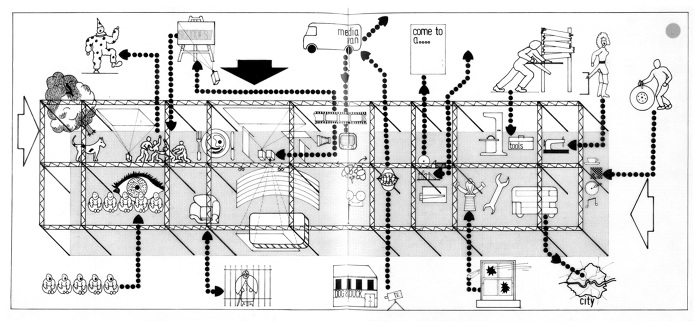
\includegraphics[width=\textwidth]{Illustrations/fun_palace.png}
    \caption[Fun Palace, (1961)]{Cedric Price's brainchild ... }
    \label{fun_palace}
\end{figure}

%%%%%%%%%%%%%%%%%%%%%%%%%%%%%

This novel approach to programmed architecture was used by many architects from then on.
Rogers and Piano proposal for the \textit{Centre Pompidou} (1971) \index{Centre Pompidou (1971)} manifested Cedric Prices Fun Palace 
designed a transparent machine with a giant screen on the main facade broadcasting electronic messages about events in the centre or cultural or political news.
first example of technology mediated interactions in connection with architecture
back the screen idea was never realised
today we have media facades everywhere

%%%%%%%%%%%%%%%%%%%%%%%%%%%%%

\begin{figure} [h!]
    \centering
        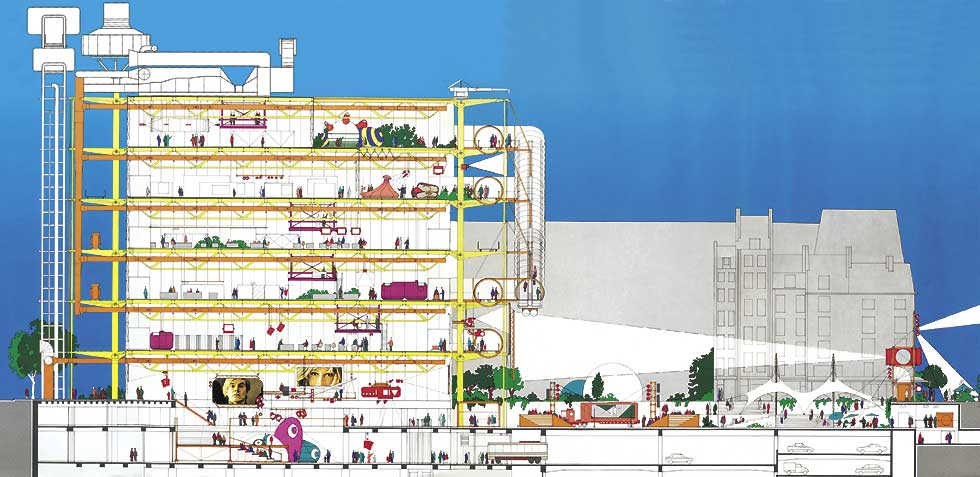
\includegraphics[width=\textwidth]{Illustrations/centre_pompidou.jpg}
    \caption[Centre Pompidou,(1971)]{An initial design drawing sketches imagines a building projection (marked through a white cone) onto the main facade in front of the main plaza. Smaller projections were suggested indoors projecting onto the outer front.}
    \label{centre_pompidou}
\end{figure}

%%%%%%%%%%%%%%%%%%%%%%%%%%%%%


What is missing here is: Venturi, Learning from Las Vegas (1972)
Learning from Las Vegas (1972) created a healthy controversy on its appearance in 1972, calling for architects to be more receptive to the tastes and values of "common" people and less immodest in their erections of "heroic," self-aggrandizing monuments.
Quote: “The Signs, oriented towards the driver’s view, use all kinds of media simultaneously: words, pictures, architecture, sound, light. The whole and its parts are balanced to work from far and near, at day and night.”


%%%%%%%%%%%%%%%%%%%%%%%%%%%%%
\subsubsection{Architectural Lighting}

Before actually continuing with electronic surfaces I briefly discuss the topic of architectural lighting which is important to mention as it existed as a discipline long before the use of electronic surfaces.

%%%%%%%%%%%%%%%%%%%%%%%%%%%%%

\begin{figure} [h!]
    \centering
        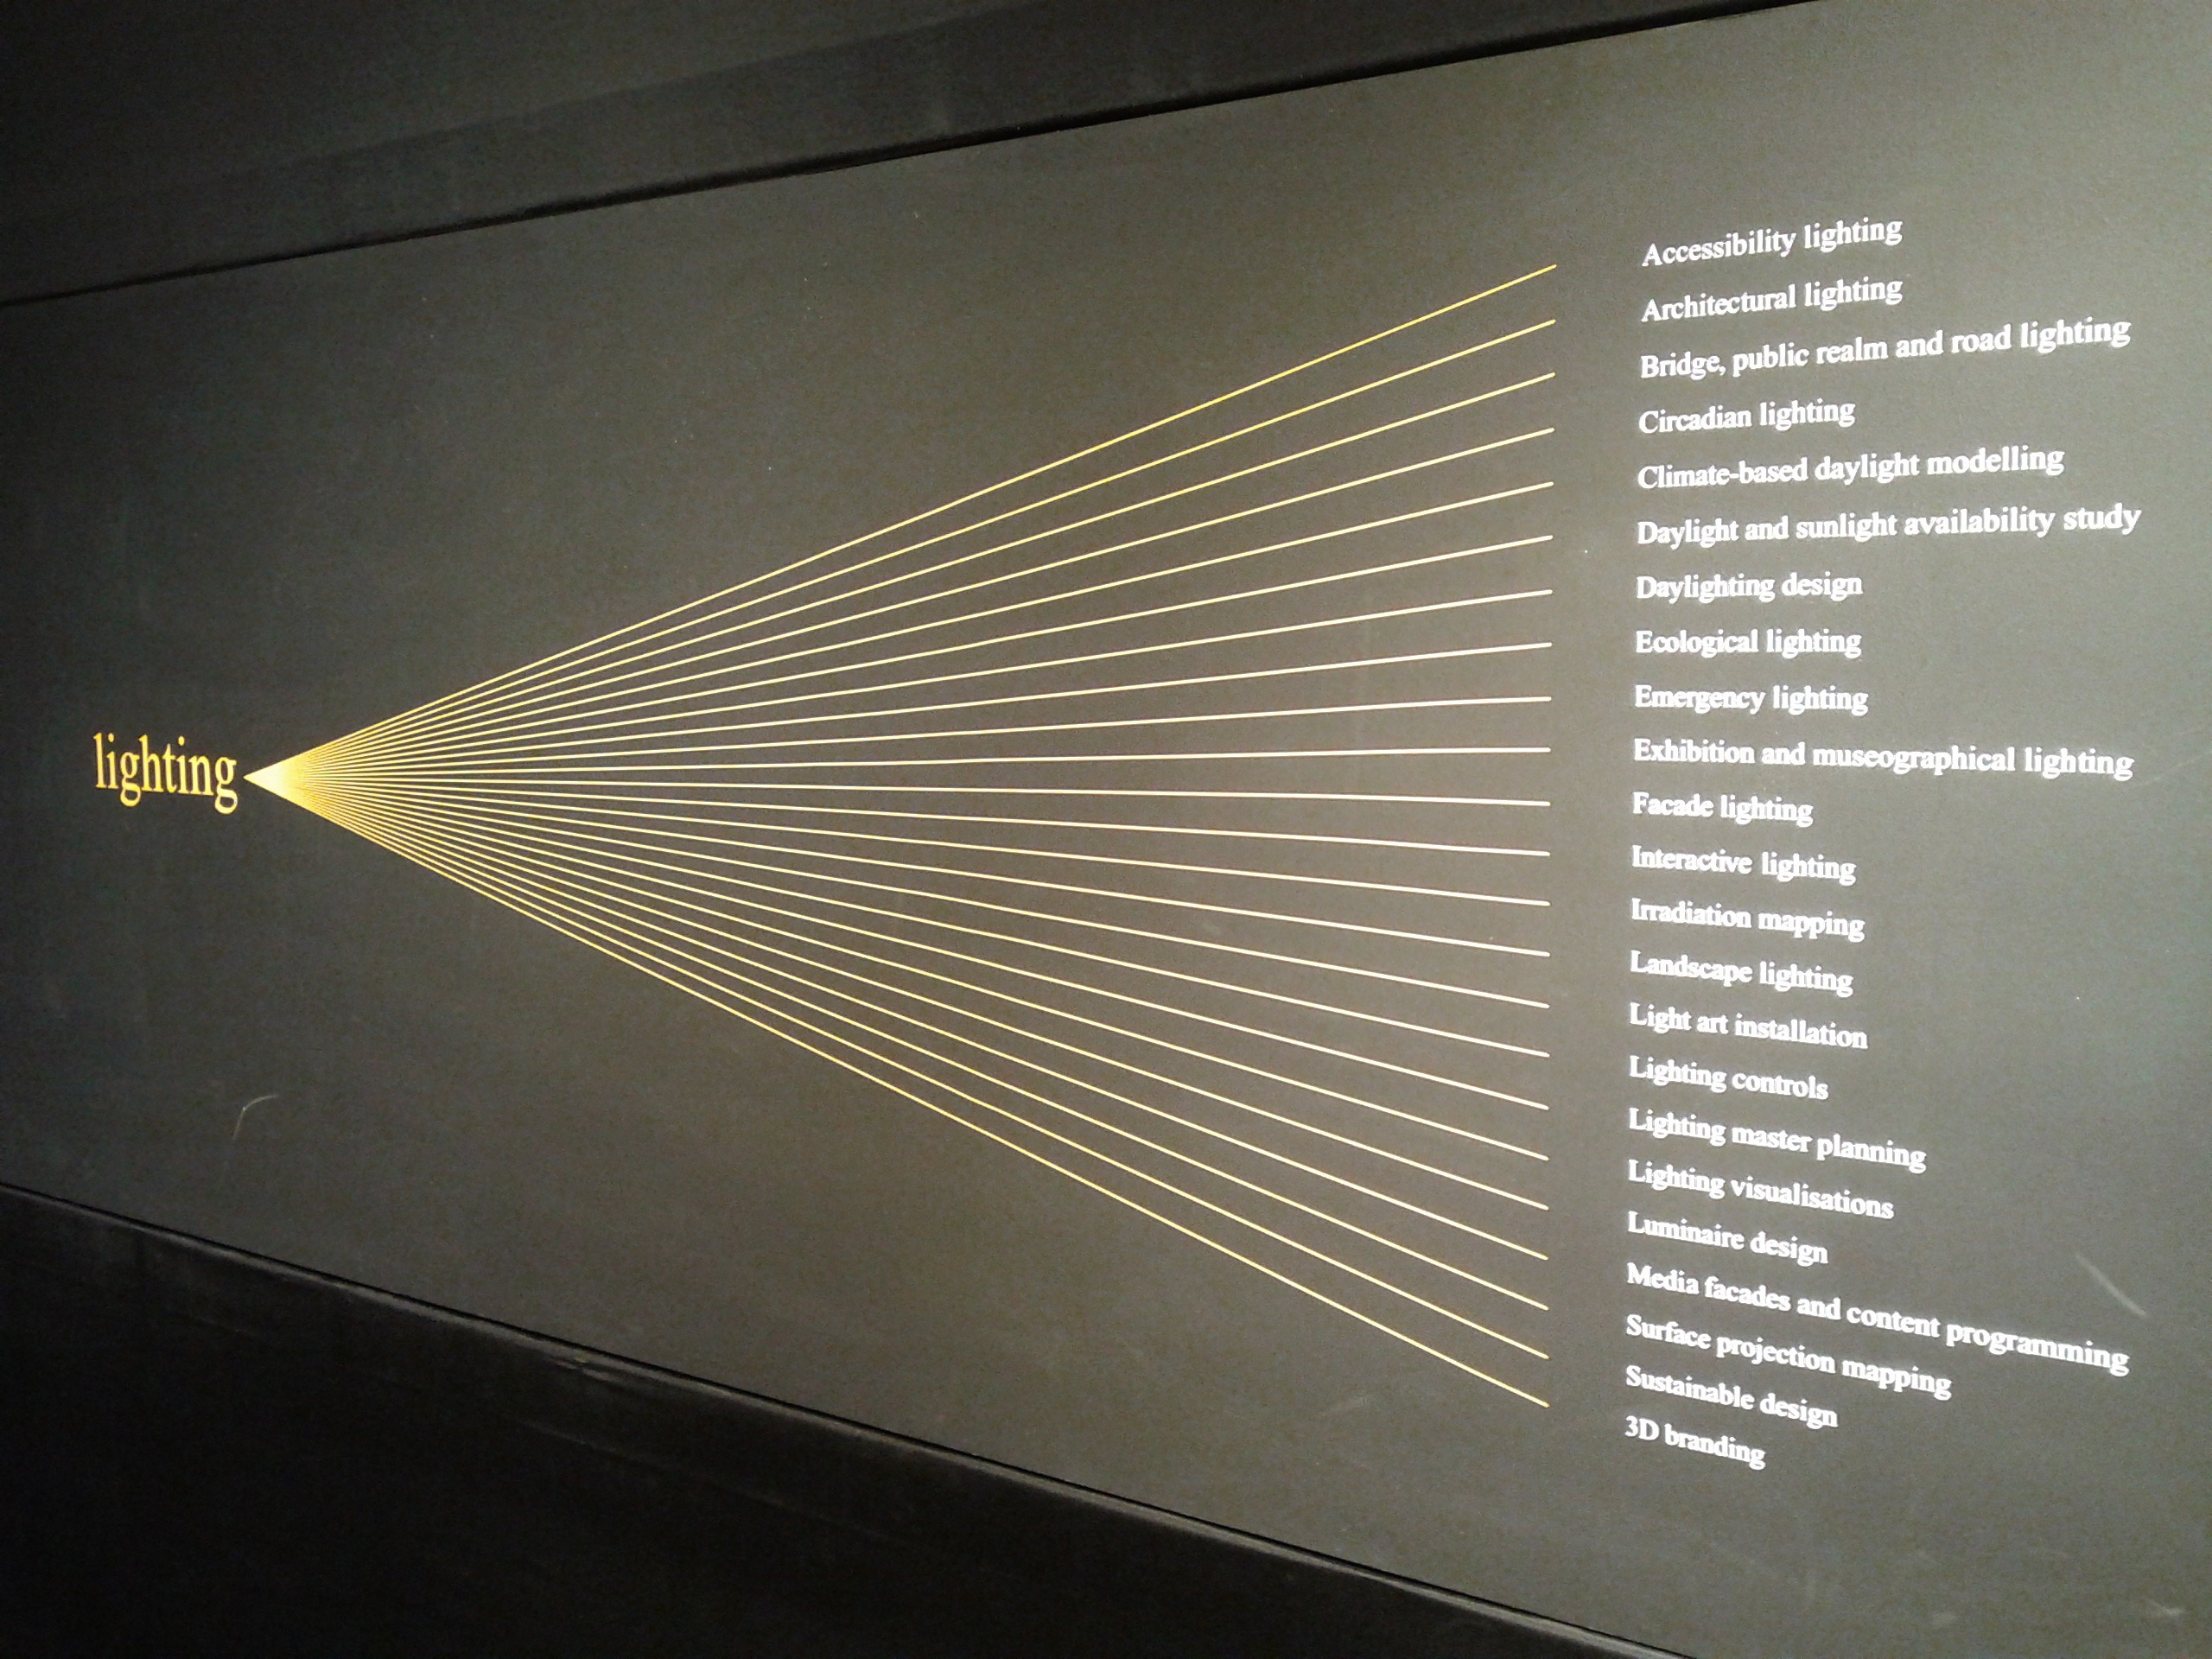
\includegraphics[width=12cm]{Illustrations/Architectural-Lighting-Fields.jpg}
    \caption[Fields of Architectural Lighting]{This diagram has been compiled by Arup for their exhibition on lighting during the international year of light in 2015 \footnote{http://www.light2015.org} }
    \label{InterfacingArchitecture}
\end{figure}

%%%%%%%%%%%%%%%%%%%%%%%%%%%%%

%%%%%%%%%%%%%%%%%%%%%%%%%%%%%

\subsection{Facade as Medium}

When it comes to architecture the notion of a building's front has always had an informational value - although static. A facade was considered to be an interface that connects the bourgeoisie (private space) with the surrounding city (public space) (Neumeyer, 2002). Architectural facades \index{architectural facade} have always been information carriers. (Architecture as a Mass Medium,  Renato De Fusco 1967)
In McLuhan's understanding traditional building materials such as bricks and stones are the medium out of which ornaments and sculptures are formed to communicate the building owner's profession or social status. 
When new media technologies emerged new types of facades emerged \cite{Haeusler2009}. Amongst those light-emitting diodes (LED) appeared as a material to build (dynamic) light facades. 
Building envelopes turned into large programmable pixel matrices displaying animated visual patterns. Information is literally not set in stone any more. 
On the contrary one can argue that new media technologies as a material in architecture has led to an arbitrary and constant exchange of information and as such can lead to a loss of identity of the built environment. Identity of place is an important feature in designing functional public spaces (see \ref{placemaking}). 

At the same time the nature of anytime and anywhere information access changed the relation between the public and private spaces which led to the development of novel forms of interactions between humans and humans, humans and computers and humans and architecture. Whereas Manovich clearly states that HCI is interactive per se (Manovich, 1991, p.71), architecture is not yet. A scale of interactivity has been described by Fritsch and Brynskov (2011) and extended by Caldwell et al. (2014).

%Manovich suggests to have a look at computer science to understand what is media today.
%To understand the logic of new media we need to turn to computer science. It is there that we may expect to find the new terms, categories and operations which characterize media which became programmable. From media studies, we move to something which can be called software studies; from media theory — to software theory.

Meanwhile, digital media technology has been weaved into buildings’ surfaces. 
For instance, visually animated surfaces, such as dynamic light facades, have been equipped with numerous addressable light-emitting diodes (LED). The FIESP building in Sao Paulo, which will be discussed in detail in the case study, is fitted with such a façade. 
Only recently the iconic 1970s building on Avenida Paulista was extended by a large programmable pixel matrix, which displays animated visual patterns. 
From a technical perspective there are other types of large electronic surfaces as well, such as projections onto facades (i.e. building projections), DIY displays, urban screens, media facades or media architectures, which I will discuss in detail in the next section.

%%%%%%%%%%%%%%%%%%%%%%

% - pre-historic cave paintings - Semper
%- Critique about the mere visual sense in today's production of architecture: Media architecture – participation through the senses Katarzyna Urbanowicz
%- In this respect the visual dominance of the visual senses have to be mentioned here. Juhani Pallasmaa (2005, 10) in his book “The Eyes of the Skin”, aims “to create a conceptual short circuit between the dominant sense of vision and the suppressed sense modality of touch.” In a way this aim is summarising the idea of interactive media architecture in my dissertation. 
%- dynamic light facades, that are equipped with numerous light-emitting diodes (LED). They turn into large programmable pixel matrices displaying animated visual patterns \cite{Haeusler2009}. 
%- today we aim to merge the digital technologies with the physical structures to enhance the urban experience  
%- "In a certain sense, the screen became the last wall. No wall out of stone, but of screens showing images. The actual boundary is the screen."  Paul Virilio, 1993 in an  interview with ‘Architecture in the Age of its Virtual Disappearance’

%%%%%%%%%%%%%%%%%%%%%%


\subsection{Large Electronic Surfaces}

Large programmable electronic displays such as building projections, urban screens, media facades and media architecture are increasingly dominating the mediascape of our cities for various purposes such as information communication, navigation, advertising and occasionally for media art. 
Today it seems that due to their omnipresence large programmable displays need to go beyond commercial purposes to stand out and create value.
At the same time electronic surfaces became a material to support architectural concepts and to implement structures. Price decline allows non-commercial initiatives to embed displays for their purposes. 
In this respect the EU funded Connecting Cities Network (CCN) established an ecology of test beds that connects various electronic surfaces and their stakeholders around the globe with enthusiastic media technologists and artists. 
Consequently, this novel synergy offers a unique opportunity for contemporary media art to explore novel socio-technological practices in urban spaces. 
It is a promising prospect to regain urban public space as the participatory domain within our cities. 
In this, novel digital technologies may support participation and media art is spearheading the exploration into interactive systems that may evoke new practices for a participatory city. 
In the following I will describe the evolution of electronic surfaces in research and practice.
I focus in particular on large programmable displays in public spaces such as public displays, urban screens, building projections, media facades or media architectures. I will consider their constituting elements potential for mediating social interactions.

%%%%%%%%%%%%%%%%%%%%%%%%%%%%%

\begin{figure} [h!]
    \centering
        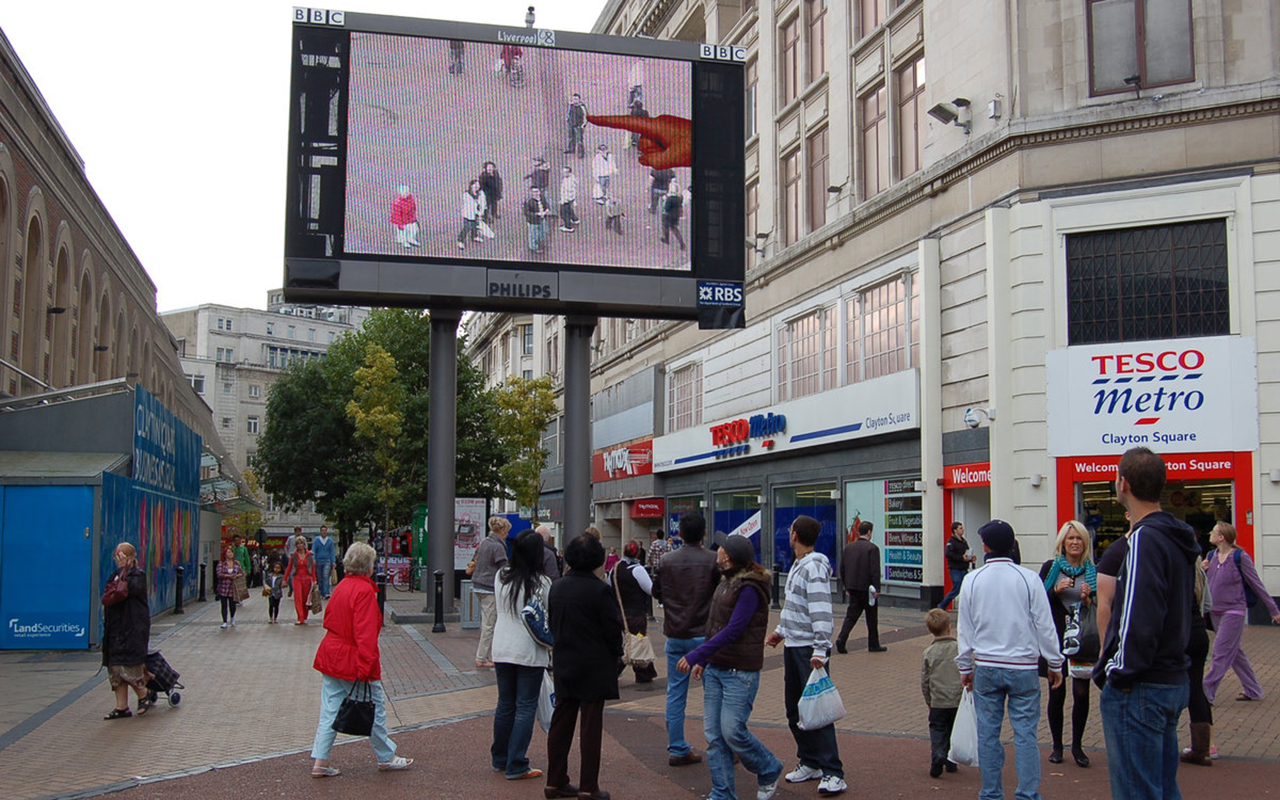
\includegraphics[width=4.5cm]{Illustrations/3.jpg}
        	%\caption[a]{Urban Screen}
      	%\label{UrbanScreen}
        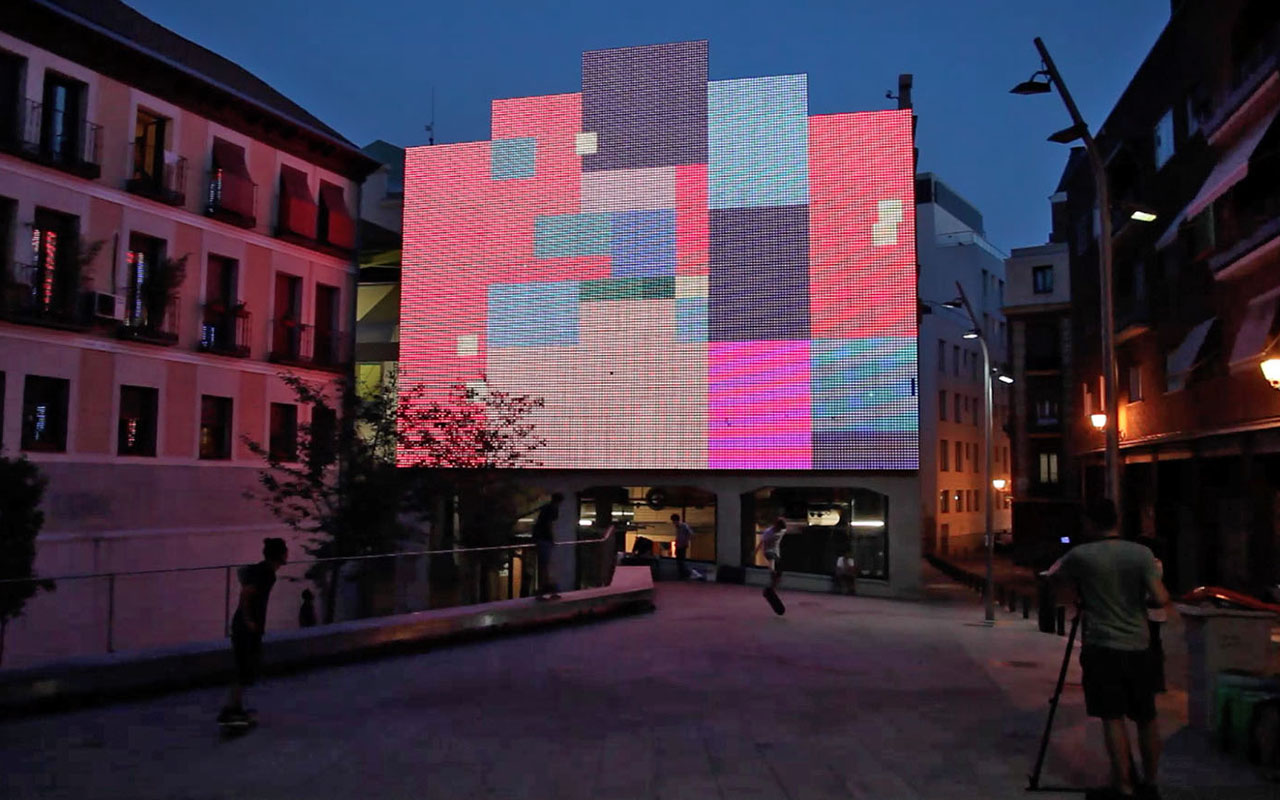
\includegraphics[width=4.5cm]{Illustrations/2.jpeg}
       		%\caption[b]{Media Facade}
       	%\label{MediaFacade}
        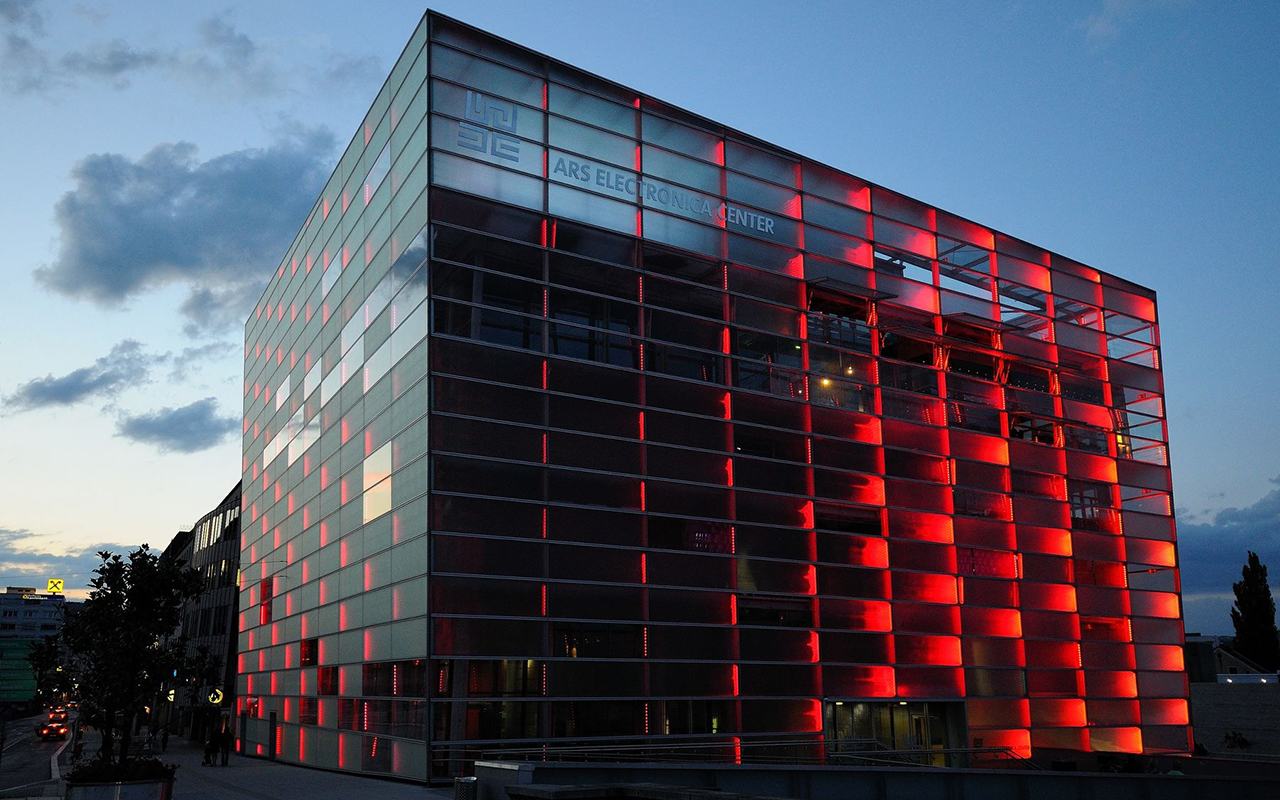
\includegraphics[width=4.5cm]{Illustrations/1.jpg}
       		%\caption[c]{Media}
     	%\label{MediaArchitecture}
    \caption[Types of electronic surfaces]{Types of large electronic surfaces in public space: (left) a free-standing rectangular urban screen, (middle) a individually shaped media facade, (right) a low resolution media architecture}
    \label{InterfacingArchitecture}
\end{figure}

%%%%%%%%%%%%%%%%%%%%%%%%%%%%%


% Please add the following required packages to your document preamble:
% \usepackage{graphicx}
\begin{table}[H]
\centering
\resizebox{\textwidth}{!}{
%\setlength{\extrarowheight}{10pt}
\setlength{\extrarowheight}{10pt}

\begin{tabular}{l|l|l|l} 
\multicolumn{1}{c|}{\textbf{Type of surface}} & \multicolumn{1}{c|}{\textbf{Surface properties}} & \multicolumn{1}{c|}{\textbf{CCN infrastructure}} & \multicolumn{1}{c}{\textbf{CCN project}} \\ \hline

\textit{Human Displays}& \begin{tabular}[c]{@{}l@{}}- embodied \\ - mobile \\ - indoors or outdoors\end{tabular} & - public space  & - 'Master/Slave Invigilator System', Jeremy Bailey (2013)  \\ \hline

\textit{Urban Screens}  & \begin{tabular}[c]{@{}l@{}}- situated \\ - permanent or temporary \\ - stand-alone or mounted\end{tabular} & \begin{tabular}[c]{@{}l@{}}- BBC Big Screen, Liverpool\\- Beşiktaş Square, Istanbul\end{tabular} & \begin{tabular}[c]{@{}l@{}}- 'Hand from Above', Chris O’Shea (2010)\\- 'Connecting Monsters', HDOTO (2013)\end{tabular}  \\ \hline

\textit{Media Facades}  &- embedded or retrofitted & \begin{tabular}[c]{@{}l@{}}- Medialab Prado, Madrid \\ - Galeria de Arte Digital do SESI-SP, Sao Paulo\end{tabular} & \begin{tabular}[c]{@{}l@{}}- ‘Sonic Skate Plaza’, Pablo Serret de Ena (2013) \\ - ‘G-Frame’, The Constitute (2014)\end{tabular}     \\ \hline

\textit{Media Architecture}  & - multi-dimensional & - Ars Electronica Centre, Linz  & \begin{tabular}[c]{@{}l@{}}- ‘Smart Citizen Sentiment Dashboard’, Behrens/Valkanova (2014)\\ - ‘(We are) Light Catchers’ Michael Ang (2015)\end{tabular}
\end{tabular}%
}
\caption[Types of electronic surfaces in urban space]{Types of electronic surfaces in urban space demonstrated through selected projects from the CC Network.}
\label{tab:typesofsurfaces}
\end{table}

%%%%%%%%%%%%%%%%%%%%%%%%%%%%%

% Please add the following required packages to your document preamble:
% \usepackage{graphicx}
%\begin{table}[]
%\centering
%\resizebox{\textwidth}{!}{
%\setlength{\extrarowheight}{10pt}

%\begin{tabular}{l|l|l|l|l}
%surface & \textbf{Human Display} & \textbf{Urban Screen} & \textbf{Media Facade} & \textbf{Media Architecture} \\ \hline
%properties & \begin{tabular}[c]{@{}l@{}}- embodied\\ - mobile\\ - indoors or outdoors\end{tabular} & \begin{tabular}[c]{@{}l@{}}- situated\\ - permanent or temporary\\ - stand-alone or mounted\end{tabular} & - embedded or retrofitted & - multi-dimensional \\ \hline

%infrastructure & \begin{tabular}[c]{@{}l@{}} - public space \end{tabular} & \begin{tabular}[c]{@{}l@{}}- BBC Big Screen, Liverpool\\ - Beşiktaş %Square, Istanbul\end{tabular} & - Galeria de Arte Digital do SESI-SP, Sao Paulo & - Ars Electronica Centre, Linz  \\ - Media Lab Prado \\ \hline

%project & \begin{tabular}[c]{@{}l@{}} 'Master/Slave Invigilator System', Jeremy Bailey (2013) \end{tabular} & \begin{tabular}[c]{@{}l@{}}- 'Hand from Above', Chris O’Shea (2010)\\ - 'Connecting Monsters', HDOTO (2013)\end{tabular} & - ‘Sonic Skate Plaza’, Pablo Serret de Ena (2013)\\ - ‘G-Frame’, The Constitute (2014)- ‘Smart Citizen Sentiment Dashboard’, Behrens/Valkanova (2014)\\ - ‘(We are) Light Catchers’ Michael Ang (2015) \\ \hline

%\end{tabular}%
%}
%\caption{My caption}
%\label{my-label}
%\end{table}

%%%%%%%%%%%%%%%%%%%%%%%%%%%%%

%\begin{figure}[!h] 
%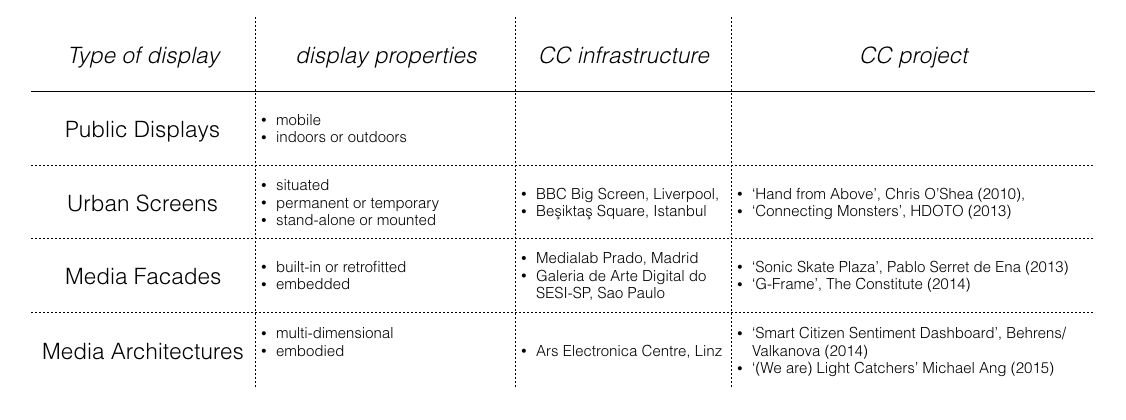
\includegraphics[width=\textwidth]{Illustrations/Types-of-displays.png}
%\caption{Types of displays}
%\label{fig:lion}
%\end{figure}

%%%%%%%%%%%%%%%%%%%%%%%%%%%%%%

\subsubsection{DIY Displays and Temporary Media Architectural Installations}

A specific application of media architecture that allows for a more experimental approach towards the exploration of new electronic surfaces are temporary media architectural installations. Due to their temporary implementation they are excluded from sometimes cumbersome processes.

\begin{itemize}
\item "Lichtwolke" - Raumwelten \index{Lichtwolke - Raumwelten (2016)} is a temporary blow-up structure that even allows for people to inhabit the structure 
\item  \textit{SKUM} \index{SKUM (2016)} by BIG architects = "inflatable balloon pavilion by bjarke ingels group / BIG. named ‘SKUM’ – the danish word for ‘foam’ – the playful and bubble form was first erected at the roskilde festival and uses the same material as bouncy castles" (taken from website).
\end{itemize}

The projects I have developed within the scope of this dissertation can be considered as temporary media architecture. They allow to be of structural and architectural nature but at the same time - through their temporarity - they give a maximum of experimental and prototypical flexibility. 


With a rapid price decline and the development of open-source platforms that provide easy to learn software tools such as Processing and Arduino computational designing became more accessible for non-experts 

With the advent of the www knowledge spread and made available more easily. Online platforms and communities provide, exchange and create new knowledge accessible for laypeople. Today we can easily find answers on how-to-fix problems, get instructions on how to do-it-yourself (DIY) or join a community and do-it-with-others (DIWO) . DIY and the maker movement not only became an alternative to consumerism but also for researchers and designers to enter new domains or to integrate digital technologies into their design work.  
One of those domains include urban computing technologies and media such as public displays. 
Access to DIY cultures and knowledge in the context of networked public displays has been used to explore community engagement by a collaboration between researchers from UCL The Bartlett and the Mixed Reality Lab at the University of Nottingham in the EPSRC funded Screens-in-the-Wild \index{Screens in the Wild (2011)} project. 
%(Considering communities, diversity and the production of locality in the Design of Networked Urban Screens by Wallis Motta https://www.irit.fr/recherches/ICS/events/conferences/interact2013/papers/8117312.pdf)

DIY Media Architectures have been explored by Caldwell et al. (2014) (DIY media architecture: Open and participatory approaches to community engagement. Caldwell, Glenda Amayo ; Foth, Marcus (2014)) 
They categorised DIY maker cultures with respect to media architectures into three categories, namely, \textit{technical DIY} which refers to the maker cultures themselves, \textit{spatial DIY}, which describe "urban interventions for the purpose of appropriating public spaces to assist in civic engagement, the communication of often political messages, or to simply improve the quality and experience of a place." (Caldwell et al.) and can be summarised with the term placemaking. The third category is called \textit{social DIY}, which they summarize as urban citizenship.

Recent projects that include DIY displays include. I have categorised them following the framework Caldwell et al. suggested:

\begin{itemize}
\item Heart of the City http://www.connectingcities.net/project/heart-city
\item (WE ARE) LIGHT CATCHERS http://www.connectingcities.net/project/we-are-light-catchers
\end{itemize}

%%%%%%%%%%%%%%%%%%%%%%%%%%%%%

Different kind of display - so called drone displays - has been explored by Ars Electronica in the project \textit{Spaxels} \index{Spaxels} \index{Ars Electronica} \footnote{\url{http://www.spaxels.at/} accessed 07.12.2016}

%%%%%%%%%%%%%%%%%%%%%%%%%%

\begin{figure}[htp]
\centering
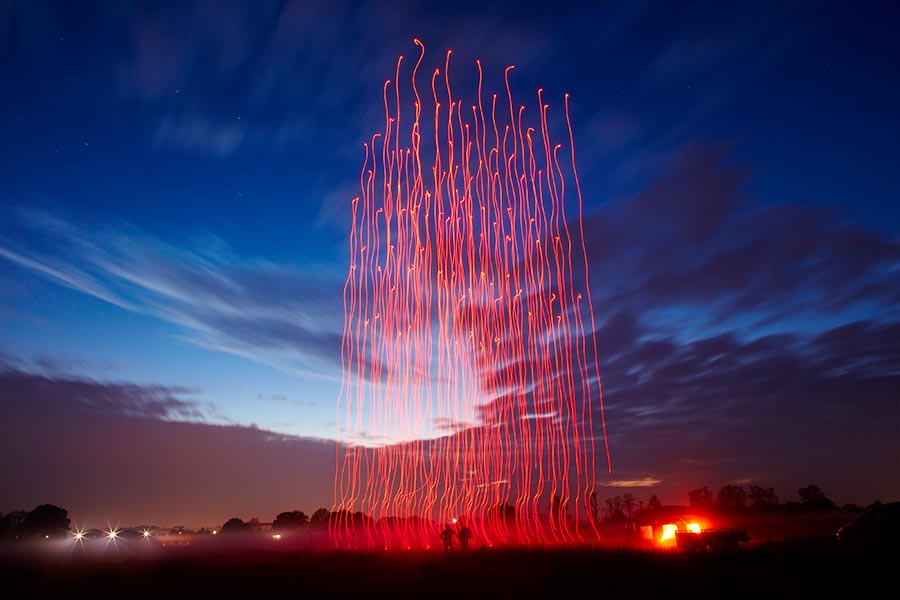
\includegraphics[width=\textwidth]{Illustrations/spaxels.jpg}
\caption{A series of drones equipped with LED pixels form a dynamic display.}
\label{spaxels}
\end{figure}

%%%%%%%%%%%%%%%%%%%%%%%%%%

The VEIV display that is part of the case study in this dissertation can be described as an DIY display. The purpose was to test an idea in an affordable time and cost frame, without specific knowledge. Based on the observations of the implementation I was able to develop a research proposal for this PhD.

DIY practices may encourage digital literacy amongst citizens in the smart city at the same time they allow interdisciplinary research. 

%%%%%%%%%%%%%%%%%%%%%%%%%%%%%%


\subsubsection{Building Projections}

For the initial proposal of the Centre Pompidou \index{Centre Pompidou (1971)} in 1971 Rogers and Piano envisioned a large projection onto the main facade of the cultural centre announcing the programme of what is going on inside (Fig.\ref{centre_pompidou}).  

Building projections map dynamic content onto existing architectural facades by means of an optical device that projects (animated) images onto a surface. Projection mappings are mostly temporary and designed for special occasions. They aim to augment architectural facades with additional dynamic visual content - mostly with a strong narrative.  

Large building projections became popular among light festivals where historic iconic building facades such as churches are overlayed with colourful patterns. Currently the biggest of these nocturnal events is the VIVID Light Festival in Sydney, Australia, where each year millions of visitors are fascinated by the various light shows and building projections produced with the latest projection technology. Light festivals in the meanwhile belong to the repertoire of global city marketing hence many major city is organising an annual festival. The first festival of this kind emerged in the French city of Lyon \footnote{Since 1852 the citizens of the French city Lyon are coming together to celebrate the unity of their city with a light festival called La Fete des Lumieres. Back then candle lights were positioned in each window. Since 1999 a professional light festival attracts many tourists in Dezember to visit Lyon. See also: \url{http://www.fetedeslumieres.lyon.fr/en/page/history} accessed 04.11.2016}.    

A building projection project worth mentioning here is the \textit{555 KUBIK} \index{555 KUBIK (2009)} project initiated by the German based \textit{Urbanscreen} agency for the facade of the Hamburger Kunsthalle, Galerie der Gegenwart in 2009 \footnote{\url{http://www.urbanscreen.com/555-kubik/} accessed 10.11.2016}. The content of full facade projection successfully plays with the existing architectural surface.  

%%%%%%%%%%%%%%%%%%%%%%%%%%

\begin{singlespace}
	\leftskip2.3em
		\rightskip\leftskip
\textit{\small The Basic idea of narration was to dissolve and break through the strict architecture of O. M. Ungers “Galerie der Gegenwart”.
Resultant permeability of the solid facade uncovers different interpretations of conception, geometry and aesthetics expressed through graphics and movement. A situation of reflexivity evolves – describing the constitution and spacious perception of this location by means of the building itself.} 

\small Project description by Urbanscreens
\end{singlespace}

%%%%%%%%%%%%%%%%%%%%%%%%%%

What is interesting here is that the designers of the projection content were playing with the rigid design grid O.M. Ungers is famous for. The rigid facade was augmented through the projection. In contrast to many other building projections here the augmented content and the original facade seemed to merge and graphical additions seemed to extend the facade.

%%%%%%%%%%%%%%%%%%%%%%%%%%

\begin{figure}[htp]
\centering
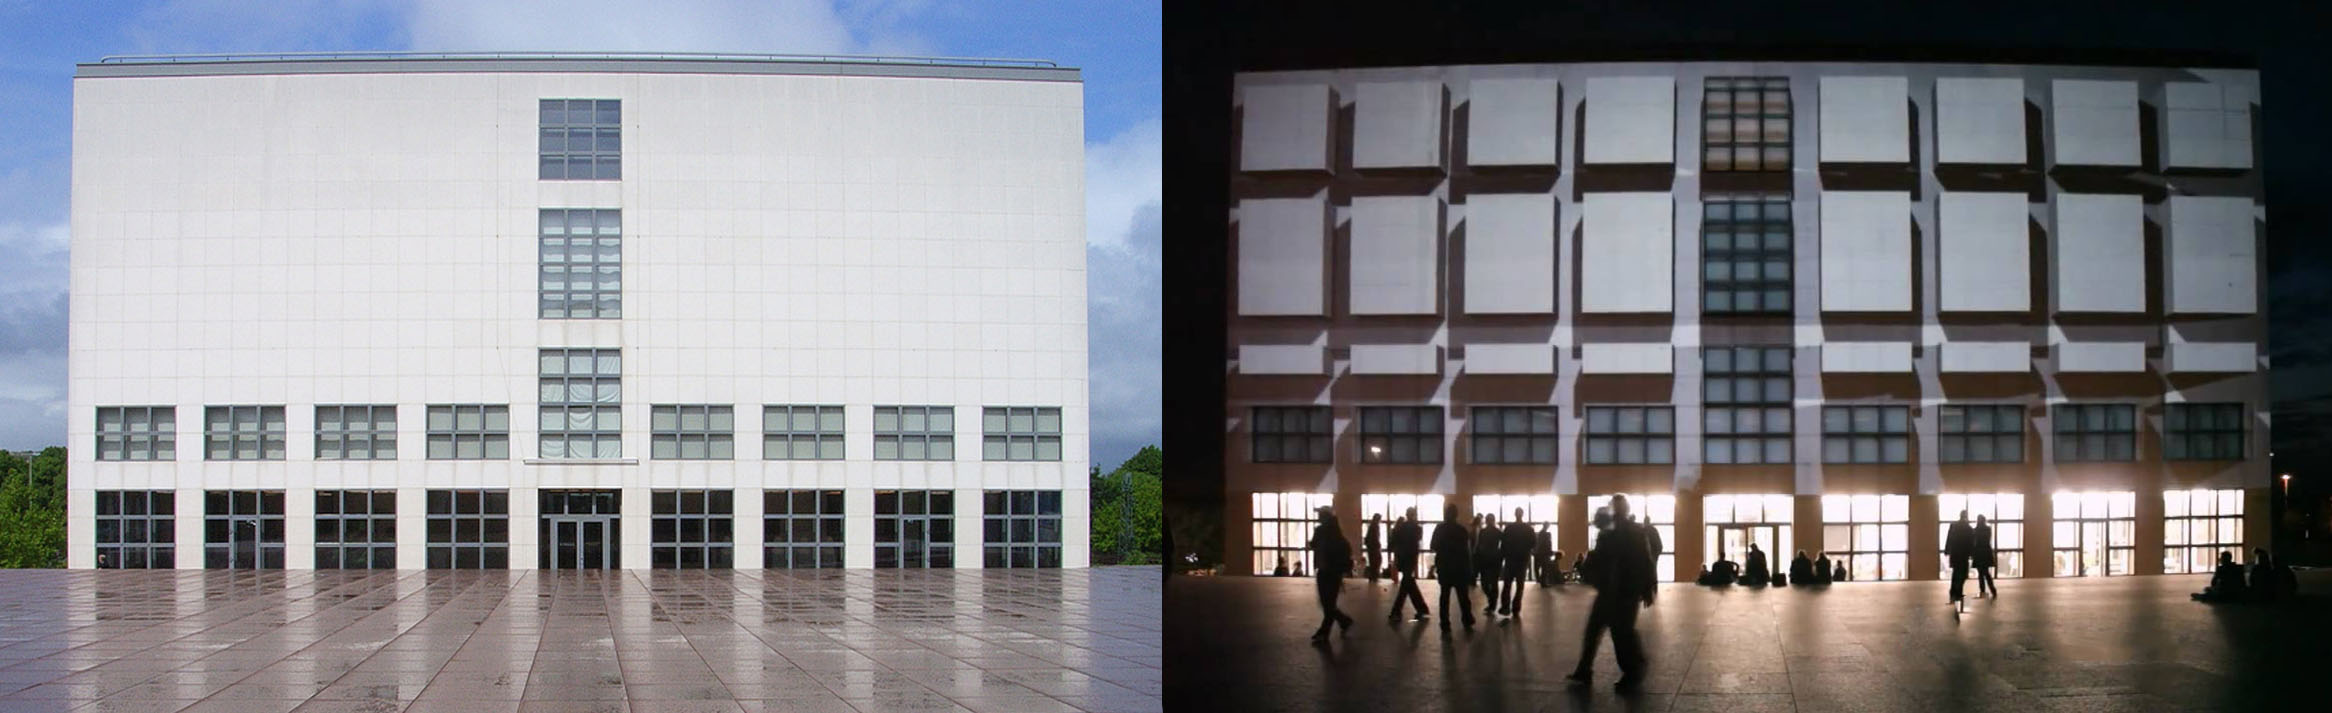
\includegraphics[width=\textwidth]{Illustrations/Ungers_day_night.jpg}
\caption{Augmentation of an architectural facade through a projection. The dynamic content allows for a speculative extension of the given surface.}
\label{fig:ungers}
\end{figure}

%%%%%%%%%%%%%%%%%%%%%%%%%%

Besides the common facade mappings there are a few so called rear-projections, that project content onto translucent film from the back. An installation that has been developed permanently and has been part of the initial architectural design process is the Media Wall.
The Media Wall in the IAC Building in New York designed by Frank Gehry and completed in 2007 is built into the reception area. 
Its dimensions are 3.4 meters high and 37 meters long. 
The projectors are based on Laser Phosphor Display (LPD) technology \footnote{ \url{http://www.prysm.com/laser-phosphor-display accessed 10.11.2016}}
Thin laminated film sandwiched between glass panels enable high resolution that compared to LED displays allows for very close use of participants.
This rear projection project is different to others and mentioned here as it is not a temporary installation with a removable support structure. The project had to be integrated into the building structure itself early on. The section Fig .. shows the backstage of the display wall with scaffolding, mirrors and projectors.

Content wise projection mappings do not always serve merely the purpose to entertain an audience with colourful and flashy animation as widely demonstrated in light festivals.   
Political activism was first explored through projections by pioneering artist Krzysztof Wodiczko, who projected a swastika on the South Africa  embassy  in Trafalgar Square London in 1985 to confront former PM Thatcher over financially supporting the  apartheid regime. Although the projection lasted only two hours the impact and media coverage has been overwhelming.     
During the 2011 Occupy Wall Street protests building projections have been used by the New York activist group The Illuminator \footnote{\url{http://theilluminator.org/about/}} to map the movements 99percent logo onto the iconic Verizon building. 

%%%%%%%%%%%%%%%%%%%%%%%%%%

\begin{singlespace}
	\leftskip2.3em
		\rightskip\leftskip
\textit{\small "99\% / MIC CHECK! / LOOK AROUND / YOU ARE A PART / OF A GLOBAL UPRISING / WE ARE A CRY / FROM THE HEART / OF THE WORLD / WE ARE UNSTOPPABLE / ANOTHER WORLD IS POSSIBLE / HAPPY BIRTHDAY / \#OCCUPY MOVEMENT / OCCUPY WALL STREET / {[list of cities, states and countries]} / OCCUPY EARTH / WE ARE WINNING / IT IS THE BEGINNING OF THE BEGINNING / DO NOT BE AFRAID / LOVE."} 

\small As the demonstration took the Brooklyn Bridge The Illuminator supported the chanting protest march with these messages.
\end{singlespace}
\
%%%%%%%%%%%%%%%%%%%%%%%%%%

The group developed a projector van, which allowed them to project the 99percent logo onto any facade in New York with ease.

Building projections can also be interactive as shown by the SMSlingshot project. Here participants were invited to shoot text messages onto a facade with the use of a slingshot.  
On another matter projections have been used for prototyping social data visualisations in favour of public engagement. Valkanova et al. (...) developed an application asking participants to reveal their energy consumption data publicly which is then projected onto a public wall. The aim is to enable rich discussions about energy consumption and behaviours.  

Projections on different surfaces: 

In summary, the small size of projectors, their high mobility and ability to be set up quickly with projecting from various angles they are highly suitable for rapid urban prototyping, bottom-up initiatives and political activism.  Consequently they have a very strong temporal aspect.
Their high resolution allow for close distant interactions.
Only occasionally the specific form of rear projections is used in permanent architectural set ups.

%%%%%%%%%%%%%%%%%%%%%%%%%%%%%

\subsubsection{Urban screens}

Urban screens are considered to be a technological advancement of the traditional billboard, serving to broadcast commercial content \cite{Huhtamo2009}. 
In the 1970s James P. Mitchell's invention of a LED (light emitting diode) matrix marked the end of the analog CRT displays (cathode-ray tube technology). This novel display technology paved the way towards today's high-resolution outdoor public displays, called urban screens.
Whilst public displays include TV sized screens in indoor places such as museums urban screens are different in scale and considered to be outdoors. 
Large programmable electronic surfaces such as urban screens can be stand-alone or façade-mounted whilst being used either temporary or permanent (Tscherteu and Tomitsch, 2011). 
%Tscherteu and Tomitsch describe urban screens as mid- to large-scale screens that can either be freestanding or attached to a building façade. (Tscherteu, G.  Tomitsch, M. (2011). Designing Urban Media Environments as Cultural Spaces. Presented at the CHI’11 Workshop on Large Urban Displays in Public Life, May 2011, Vancouver, Canada.)
In 2005 a conference was hosted in Amsterdam with the name Urban Screens. For the first time advertisers, content providers, engineers, stakeholders, researchers, architects, city planners and artists came together to discuss the future of large public displays. 
The questions considered since then were manigfold:

%%%%%%%%%%%%%%%%%%%%%%%%%%%

\begin{singlespace}
	\leftskip2.3em
		\rightskip\leftskip
\textit{\small "What is the relation between technology, culture, economics and politics? How do technical decisions, such as determining standards and ‘affordances’, or erecting stand-alone installations or forming unified networks, affect cultural experiences and the distribution of power? How should we conceptualise public participation in relation to urban screens? Are the public citizens, consumers, producers, or something else? And when considering the location of a large screen, what are the appropriate forms of urban planning, design and governance? When a screen is erected in public space, who should have access to it and who has control over it? What kinds of partnerships enable innovative screen programs, and contribute to rich public cultures? How might this be evaluated? In what conditions can public screens contribute not only to new forms of public interaction but to the deeper democratic ambi- tions of public culture? Where is the contemporary public sphere located and what are its boundaries and lines of force?"} 

\small Taken from the introduction of the Urban Screens Reader by Mcquire, S., Martin, M. and Niederer, S. 2009.
\end{singlespace}

%%%%%%%%%%%%%%%%%%%%%%%%%%%

One can mention the stand-alone and permanent \textit{BBC Big Screens} \index{BBC Big Screens} distributed across the UK. In Liverpool the Big Screen hosted a CCN project in 2010 named \textit{Hand from Above} \index{Hand from Above (2010)} by Chris O’Shea.
A similar infrastructure exists at the Beşiktaş Square in Istanbul where CCN deployed \textit{Connecting Monsters} \index{Connecting Monsters (2013)} by HDOTO in 2013. 

%%%%%%%%%%%%%%%%%%%%%%%%%%%%%

\subsubsection{Media facades}

Haeusler, M. Hank, Tomitsch, Martin,  Tscherteu, Gernot. (2013). New Media Facades: A Global
Survey. Ludwigsburg, Germany: avedition.

Another type of large electronic displays constitutes media facades. Here digital media technology is already built-into the building’s surface or retrofitted to an already existing building. An example where the installation of a media facade was already part of the initial design process of the building is the Media Lab Prado in Madrid, Spain or the Ars Electronica Center in Linz, Austria. Whereas the iconic FIESP building in Sao Paulo, Brazil built in the 1970s only recently was retrofitted with a media facade.

Seen from building engineering, according to Tomitsch, media facades "in contrast to Urban Screens feature a closer integration of the screen and the building layers, if not a complete integration into a new hybrid structure." (Tomitsch)

Eight challenges have been identified by Dalsgaard and Halskov (2010). 
%Dalsgaard, P., & Halskov, K. (2010). Designing Urban Media Façades: Cases and Challenges. In Proceedings of the 28th international conference on Human factors in computing systems (pp. 2277–2286). ACM.
These challenges clearly acknowledge the importance of the particular physical space a media facade is planned to be implemented (i.e. Spatial Layout). Further the impact of media facades on social interactions (i.e. Movement) is mentioned, as well as the function of the media facade itself (i.e Attractor).
%%%%%%%%%%%%%%%%%%%%%%%%%%

\begin{figure}[htp]
\centering
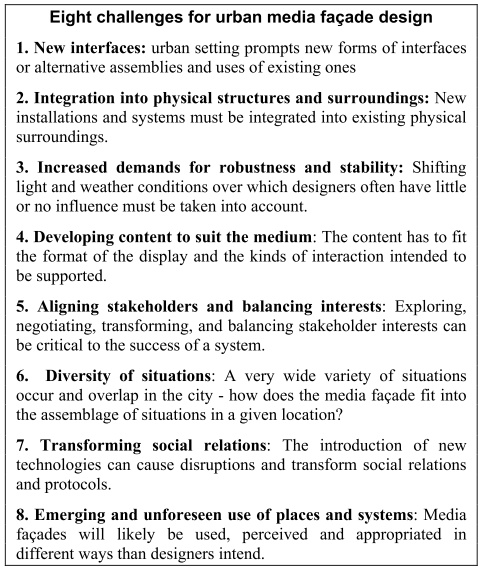
\includegraphics[width=8cm]{Illustrations/8challenges.png}
\caption[Eight challenges for urban media facade design]{Eight challenges for urban media facade design taken from }
\label{8challenges}
\end{figure}

%%%%%%%%%%%%%%%%%%%%%%%%%%

Kunsthaus Graz \index{Kunsthaus Graz - BIX (2003)}finished in 2003 is an architectural landmark designed by Archigram architect Peter Cook and Colin Fournier. 
The BIX {(acronym for Big piXels)} media facade has been designed by the Edler brothers from the Berlin based practice realities:united 
%\footnote{\url{http://www.realities-united.de/#PROJECT,69,1} accessed 11.11.2016}.
In away the BIX media facade is a retrofitted facade as well as the lighting designers have been called in only when the Kunsthaus has already been under construction. Hence in my definition it is not a media architecture. I will explain this in the next section.

The conceptual idea for the BIX media facade has been further explored in the project SPOTS \index{SPOTS (2005)}

A recent project that illustrates the idea of display technology as a material for architectural design is the \textit{LED Frieze} facade (2016) \index{LED Frieze (2016)} for the new building of the Kunstmuseum Basel designed by Christ and Gantenbein. The solid bright brick front with few openings is at the top interrupted with a luminous band of three meters hight that encricles the entire museum at a height of 12 meters. The relief like pattern of the bricks creates tiny voids that are equipped with 
The low resolution and monochromatic media facade is able to show text and patterns. From an architectural point of view this is a very successful project.
\smalltodo[size=\footnotesize]{This argument needs to be picked up in the discussion about the cocoon and its appearance ... low res and monochromatic, but very strong in its architectural expression.}
%%%%%%%%%%%%%%%%%%%%%%%%%%

\begin{figure}[htp]
\centering
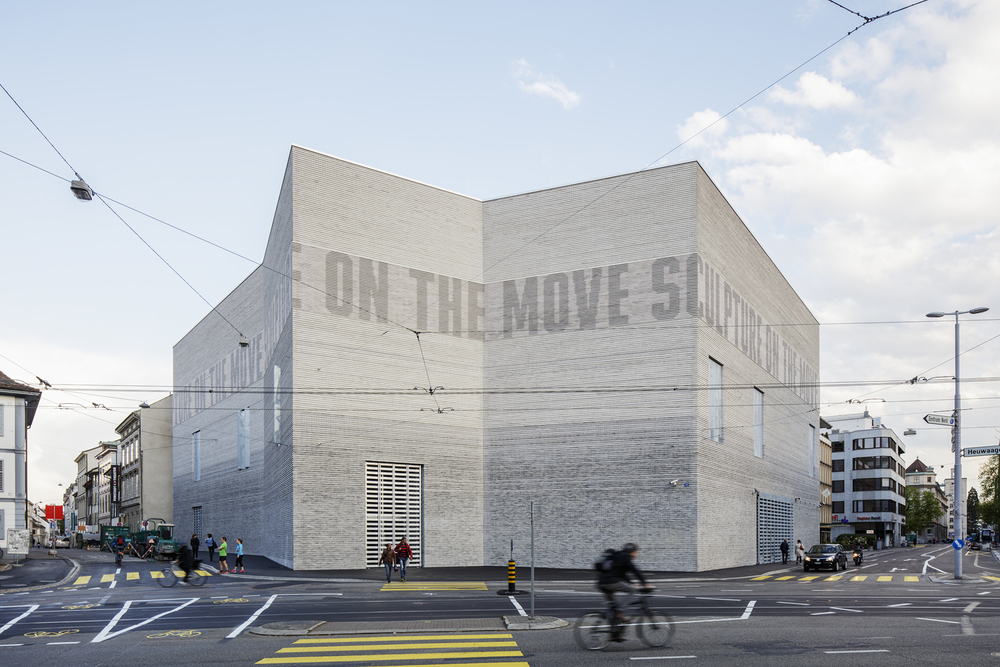
\includegraphics[width=\textwidth]{Illustrations/LEDfrieze.jpg}
\caption[LED Frieze by Christ and Gantenbein (2016)]{xxx}
\label{LEDfrieze}
\end{figure}

%%%%%%%%%%%%%%%%%%%%%%%%%%


\subsubsection{Media architecture}

Although literature in media architectural research mainly considers media architecture as an umbrella for the aforementioned surface types (i.e. DIY screens, urban screens, building projections and media facades), I argue that digital technology and media utilised for architectural design constitutes a category on its own. In the following I will developed a definition for what I consider the notion of media architecture.

In recent years different technical, spatial and social definitions gathered around the emergent term media architecture depending on which discipline is looking at it. Practitioners and researchers from architecture, lighting design, interaction design or HCI covered a wide range of social, spatial and technical aspects. 


The technical aspects with the respect to light have been summarized by Gielen: "Media architectures are technical systems consisting of a matrix of components that are able to individually change its appearance in terms of luminance and/or colour to depict digital content." 
%Johann Gielen (Lighting  Urban Designer, 2013)
The aspect of spatiality in media architectures and how it differs from the aforementioned surface types (i.e. DIY screens, urban screens, building projections and media facades) have been identified by Tomitsch: "Media installations work with the depth of space, in which case it is no longer possible to speak of a screen or a façade." 
%(Tomitsch) 

Brynskov et al. [6: p. 1-2], "Media architecture is an overarching concept that covers the design of physical spaces at architectural scale incorporating materials with dynamic properties that allow for dynamic, reactive or interactive behavior. These materials are often digital, but not always, and they allow architects and (interaction) designers to create spatial contexts for situations using a variety of modalities."
%(Brynskov, M., Dalsgaard, P.,  Halskov, K. (2013). Understanding Media Architecture (Better): One Space, Three Cases. Presented at the CHI’13 Workshop on Interactive City Lighting, Paris, France.)


I consider all these definitions as valuable under the umbrella of media architecture, however they are only describe partially the notion of media architecture. All these definitions together form the notion of media architecture. 

Consequently, media architectures manifest the idea of incorporating digital technologies and media systems already into the initial process of architectural designs by architects, designers and media artists. Here I would like to emphasise the initial intention to integrate digital technologies and media systems as materials of the architect to implement her vision. In other words, media architectures involve multi-dimensional media systems from the very beginning, and electronic surfaces become part of the architectural repertoire. The emblematic building of the Ars Electronica Centre incorporates this approach towards a museum that offers artists the platform to explore the technology mediated future not only within the building but as well on the outer media façade. 

We follow this definition in practice and hence it is part of our methodology in this research.


One can categorise Media Architecture into the following groups as defined by the Media Architecture Institute:
"The Media Architecture Awards are given to outstanding projects at the intersection of architecture, media and interaction design. Three projects are nominated in each of the five categories:

%%%%%%%%%%%%%%%%%%%%%%%%%%%%%

\begin{itemize}
\item \textbf{Animated Architecture:} Projects demonstrating creative media facades solutions
\item \textbf{Money Architecture:} Projects illuminating buildings that are closely related to business, banks, shopping centres, and entertainment.
\item \textbf{Participatory Architecture and Urban Interaction:} Interactive media projects that enable local city development from a bottom up perspective.
\item \textbf{Spatial Media Art and Future Trends and Prototypes:} Projects produced in an artistic context at the intersection of architecture and media art, mostly non-permanent movable installations with an innovative form of spatial interaction and/or perception of space.
\item \textbf{Future Trends and Prototypes:} Special solutions like three-dimensional displays, kinetic facades, OLEDs or even robotic elements that could shed light on what future media architectures might look like.
\end{itemize}



\begin{figure}[htp]
\centering
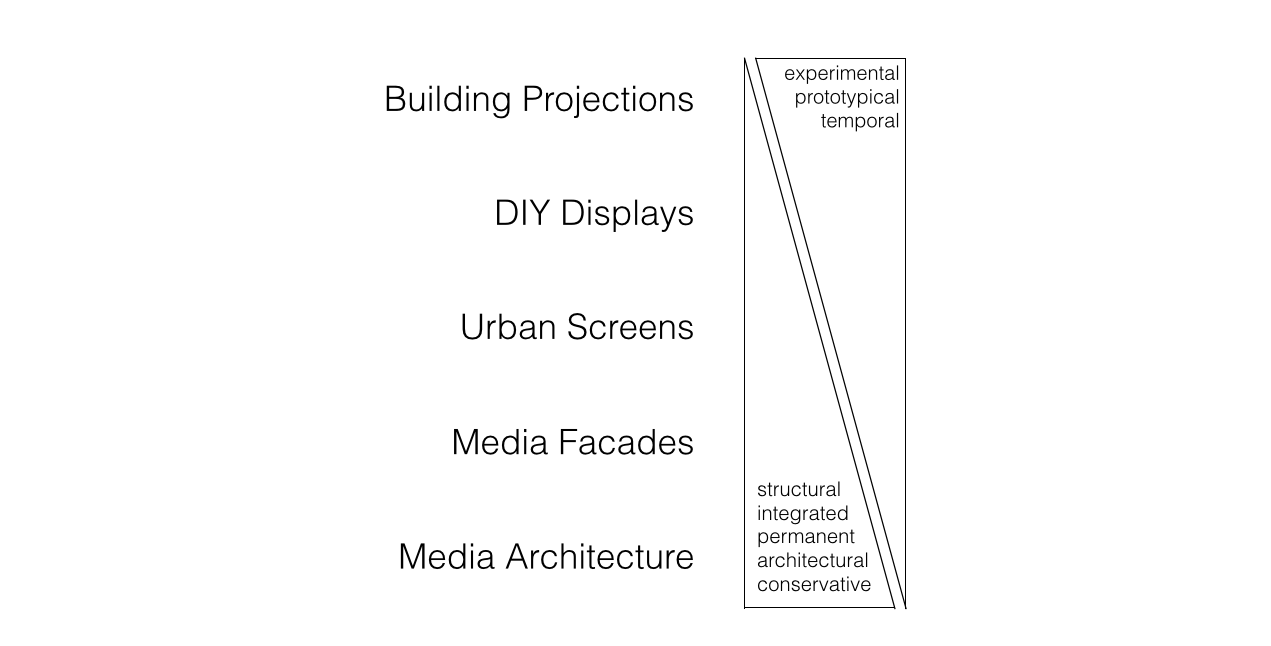
\includegraphics[width=\textwidth]{Illustrations/Typo_diagram.png}
\caption{Interactivity is missing!!! The diagram shows the properties and relations between }
\label{Typo_diagram}
\end{figure}

%%%%%%%%%%%%%%%%%%%%%%%%%%

\subsubsection{Architectural/Urban Mediascapes  / Networked Urban Mediascapes}

Definition:
Marcus Foth, Florian Fischer, Christine Satchell:From Movie Screens to Moving Screens: Mapping Qualities of New Urban Interactions, Media City 4

Projects:
- illuminated river london
- China ... ?

%%%%%%%%%%%%%%%%%%%%%%%%%%

\subsection {Media Architecture and the Role of Context}

McQuire \cite{McQuire2006} argues that TV screens have been transformed from small-scale interior devices to large architectural surfaces that no longer broadcast to private inside spaces but to public outside spaces. Architectural surfaces turned into public media interfaces, transmitting mostly content curated by corporate organisations, rather than interactions generated by the public in situ. 

Some see digital media facades as simple ornaments that create an ambient atmosphere \cite{Caspary2009}. 
Others consider the potential of digital media facades for communicating content, for instance, advertising (e.g. Times Square, New York or Piccadilly Circus, London), news content (e.g. the network of Big Screens in the UK, which was initially run by the BBC),\footnote{xxxBBCBigscreen} media art (e.g. Lozano Hemmer’s work),\footnote{xxx} social visualization (e.g. BlinkenLights)\footnote{xxx} or for community purposes on a neighbourhood level (e.g. Screens in the Wild).\footnote{xxx}

Extensive research has been carried out to explore the challenges of deploying large electronic surfaces in public space.
Initially, the technical challenges of deploying display technology in public space have been summarised by Streitz et al. \cite{Streitz2003}. 
As the design and implementation of digital media facades in the built environment progresses, the purpose of such facades and the contextual characteristics of ''media architecture" are addressed. Parameters that impact the integration of media
facades into the existing social fabric from a socio-demographic (environment), technical (content) and architectural (carrier) perspective have been addressed by Vande Moere and Wouters \cite{VandeMoere2012}. On the urban scale, the role of space, social proximity and full body performative interactions in shared spaces have been addressed by Fatah gen Schieck et al. \cite{Fatah2008}, O’Hara et al. \cite{Hara2008} and Peltonen et al. \cite{Peltonen2008}.



%%%%%%%%%%%%%%%%%%%%%%%%%%

\section{Socio-Spatial Interaction Frameworks}

In the following, I will focus on four existing frameworks that acknowledge space as an essential component when designing for mediated interactions in public space. The compilation aims to complete current HCI research about the importance of space within an integrated media architectural design. 

Only recently the spatial has been detected in HCI research:
%%%%%%%%%%%%%%%%%%%%%%%%%%

\begin{singlespace}
	\leftskip2.3em
		\rightskip\leftskip
\textit{\small (...)the fundamental character of ubiquitous computing research is not technological, but spatial. (...) the spatial character of ubiquitous computing systems is one of their intrinsic properties and a crucial area for analysis and design. 
By “spatial” here, I do not mean merely geometric. 
Instead, I am focused on the fact that they inhabit the same space as we do, and that they structure it and organize it in much the same way as our own activities and movements do.} 

\small Foreword by Paul Dourish In: Willis, K.S., Shared Encounters,
\end{singlespace}

%%%%%%%%%%%%%%%%%%%%%%%%%%


Each framework that will follow describes the relationship between humans and their action in the presence of programmable electronic displays and in relation to the surrounding space.
These frameworks describe the following: (1) awareness space, (2) actor space, (3) action space, and (4) physical space (Fig. 1).

%%%%%%%%%%%%%%%%%%%%%%%%%%%%%

\begin{figure}[htp]
\centering
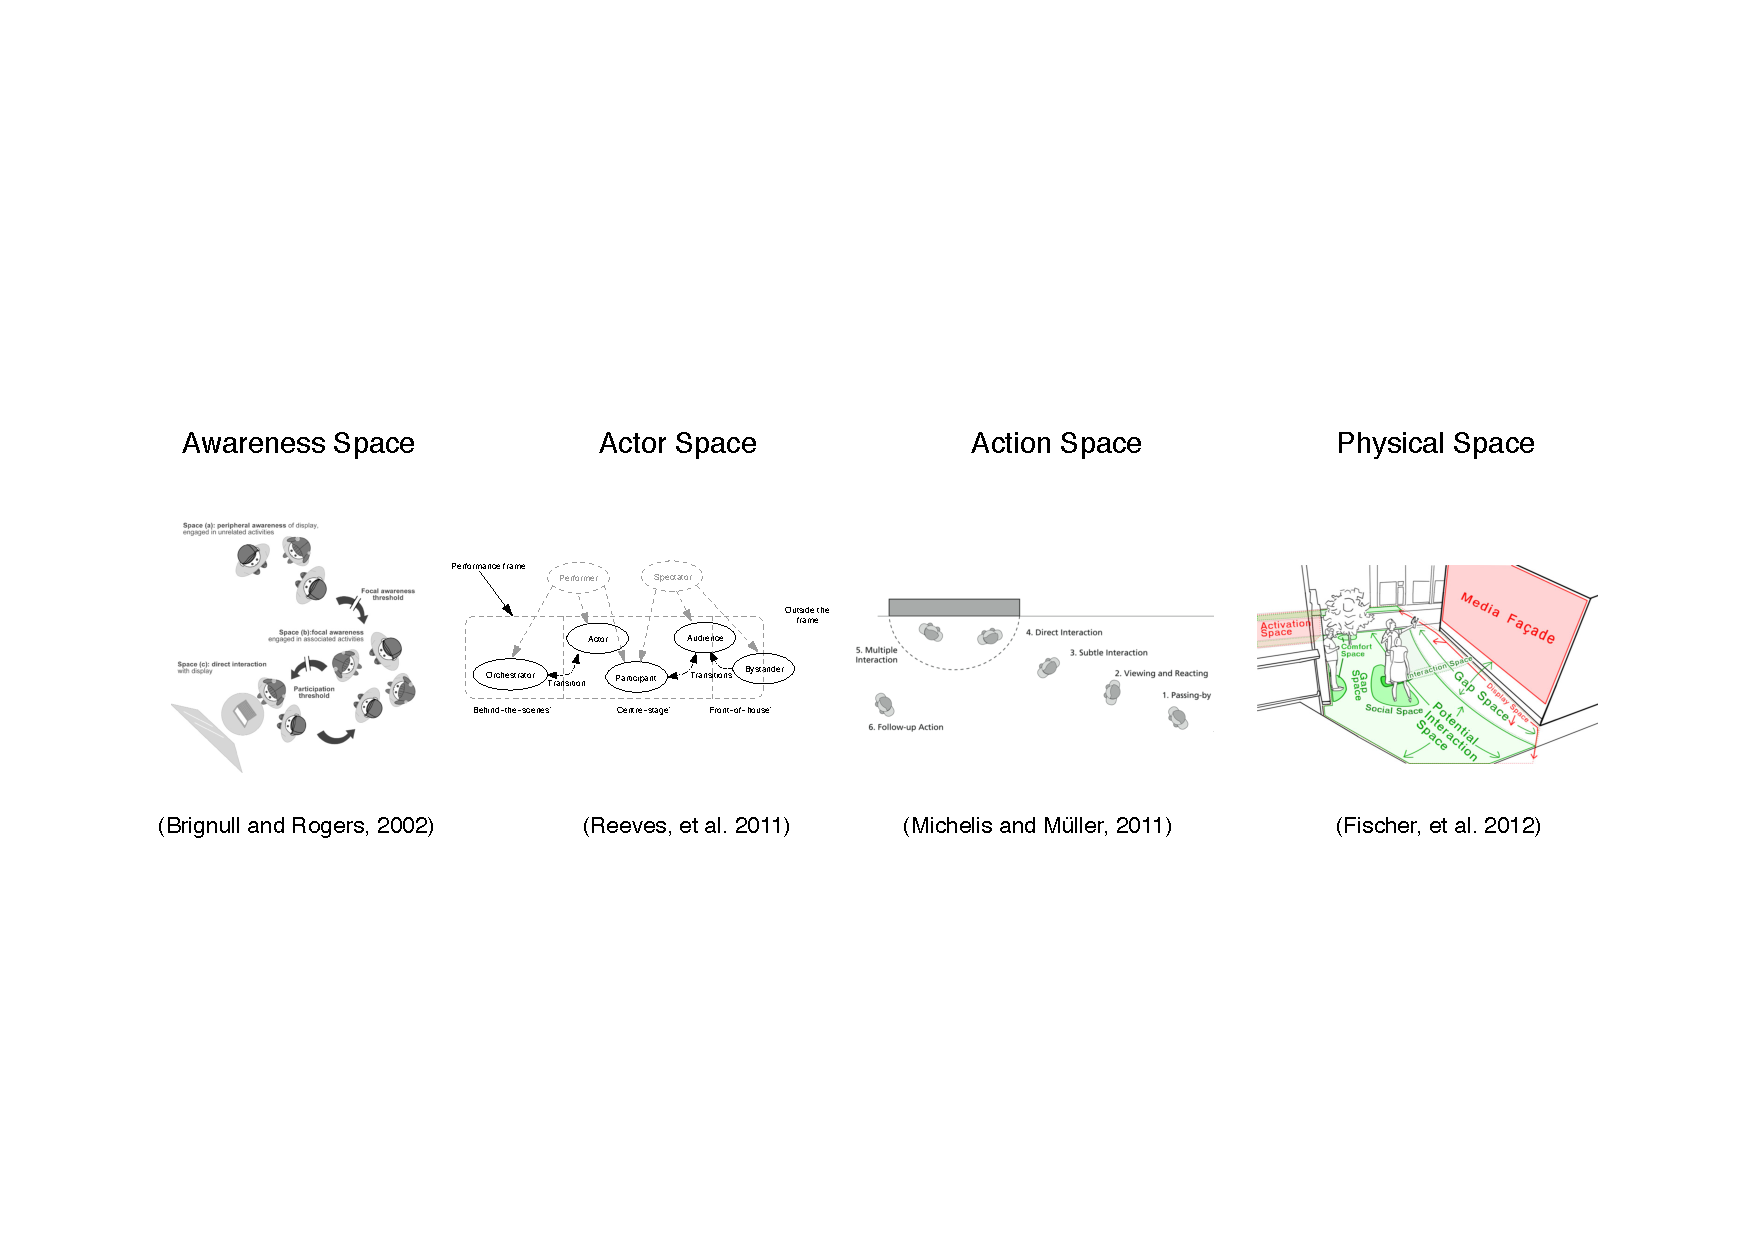
\includegraphics[width=\textwidth]{Illustrations/SpatialFrameworks.pdf}
\caption{Four existing socio-spatial interaction frameworks}
\label{fig:Background-frameworks}
\end{figure}

%%%%%%%%%%%%%%%%%%%%%%%%%%%%%

\subsection* {Awareness Space}
Research on awareness of public displays in relation to social interactions was first described in HCI research, when noticing a novel social phenomenon around public displays (Brignull and Rogers 2003). 
Three different types of ‘activity spaces’ were described: (1) Peripheral awareness activities: activities that take place in the wider space around the display, where people socialize but are not necessarily aware of the presence of the public display. (2) Focal awareness activities: in this space, people are aware of the presence of the display. 
They are looking at the display, discuss activities that take place around the display or learn how to engage with the content. (3) Direct interaction activities: this is the space where individuals or groups actively engage with the display. The research findings suggest that
people found it difficult to transit from one ‘activity space’ to another.
Later, Vogel and Balakrishnan (2004) published a spatial framework, which
described how users fluidly move from implicit interactions in the wider surrounding
towards explicit interactions when approaching the direct interaction space
around a public display.

\subsection* {Actor Space}
The actor space describes the different roles people take on when being in the vicinity of interactive installations. 
By now, computers have moved away from the desktop and novel interfaces appear, which spread into new spatial settings.
People are changing their role; in particular, in public settings people traverse various awareness spaces, which afford specific roles. 
Consequently, a better understanding of what kind of roles these are, when and where people take them on, is crucial for the design and deployment of interactive systems in urban spaces.
Reeves (2011) identified that the conventional user is actually changing her role when passing-by, on looking or turning into a performer in the vicinity of an interactive installation. 
Within this framework, the performing user plays the central role when engaging with an interface. 
Her acting entices other people from the audience into the experience; some of them may become performers. 
More recently, Behrens et al. (2013), and Fatah gen Schieck et al. (2013), have explored in detail how these roles are framed through the situated layout of urban screens.

\subsection* {Action Space}
In the last section, we clarify the diverse roles individuals take on in connection with interactive installations; here, we describe the various phases of interactions people traverse. 
The Audience Funnel by Michelis and Müller (2011) depicted a framework that establishes a terminology for each transition. 
These phases were identified as (1) passing by, (2) viewing and reacting, (3) subtle interaction, (4) direct interaction, (5) multiple interactions and (6) follow-up action. 
Michelis and Müller found that people proceed from one phase to the next in order to understand the interaction. 
Boundaries are described as a series of thresholds that need to be crossed before one can interact with a public display.

\subsection* {Physical Space}
The spatial localization of interactions is largely neglected in the work described above. 
In contrast, Fischer and Hornecker (2012) have outlined an interaction framework that focuses on the spatial properties of interactions. 
When looking into the various encounter stages, ‘urbanHCI’ specifies different ‘interaction spaces’ on which people perform different activities. 
This includes the (1) display spaces, (2) interaction spaces, (3) potential interaction spaces, (4) gap spaces, (5) social interaction space, (6) comfort space and (7) activation space on which participants
behave differently towards an interactive media facade. 
Fischer and Hornecker’s framework was explored through a media art project called ‘SMSlingshot’. 
This project developed an interface that looks like a wooden slingshot, but its integrated digital technology allows the user to shoot short text messages (SMS) together with virtual paintballs on a media facade. 
Within these immediate spaces around an electronic display (i.e. interaction spaces), passers-by stop, watch and start playing with the media architectural interface and eventually change the look of the media façade individually; others observe in groups from a distance, discuss or engage as well; simultaneously, other pedestrians do not sense the presence of such interactions and the existence of the media facade at all. 
‘Screens in the Wild’, on the other hand, addressed the question of spatial layout and its relation to technologically mediated interactions (Behrens et al. 2013; Fatah gen Schieck et al. 2013). 
Four interactive and networked urban screens have been deployed in four different neighbourhoods in London and Nottingham.
Within this approach, the following interaction zones were recognized: (1) direct interaction space surrounding the display (direct); (2) the surrounding public space (wide); and (3) across spatial boundaries, i.e. the remotely connected space through the networked displays (networked).
Sociospatial configurations mediated by urban screens were explored, and site-specific interactions were observed and compared to more generic types of interactions. 
Indications were found that the properties of the spatial layout play a significant role and, to a certain extent, frame the type of interactions mediated through public displays (Fig. 2).

In a more systematically approach the ‘Screens in the Wild’ research project explored socio-spatial configurations mediated by urban screens (Behrens et al. 2013, Fatah et al. 2013). Within this research project four interactive and networked urban screens have been deployed in four different neighbourhoods in London and Nottingham. The particular study the applied methodology, included the analysis of the spatial layout in two screen locations in London. This was followed by the observations of social behaviour and technologically mediated interactions by actors, spectators and passers-by during two community events. Within this study the following interaction zones were recognized: 1) direct interaction space surrounding the display (direct); 2) the surrounding public space (wide); and 3) across spatial boundaries i.e. the remotely connected space through networked displays (connected) over time. Site-specific interactions were observed and compared to more generic types of interactions. Indications were found, that the properties of the spatial layout play a significant role and, to a certain extent, frame the type of interactions mediated through public displays (fig. 34).

%%%%%%%%%%%%%%%%%%%%%%%%%%%%%

\begin{figure}[htp]
\centering
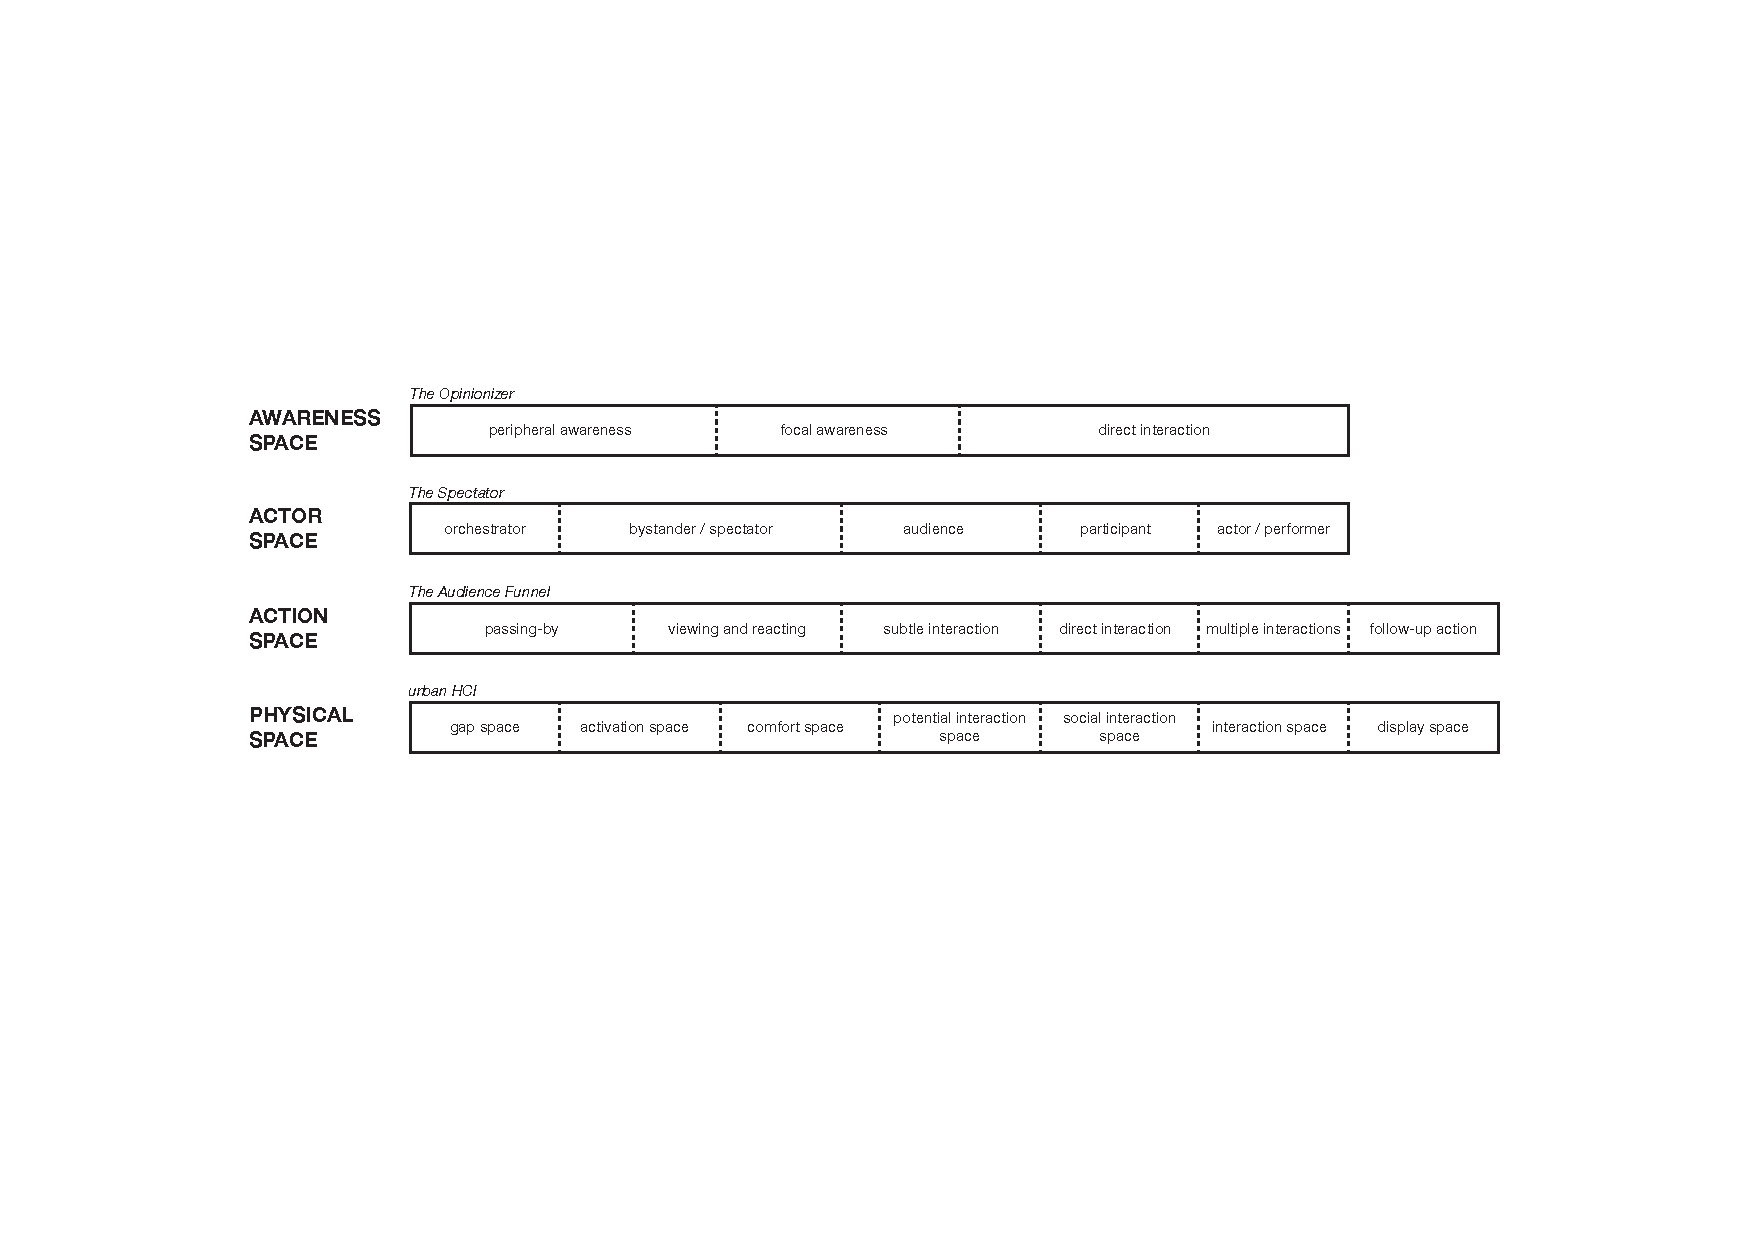
\includegraphics[width=\textwidth]{Illustrations/SpatialFrameworks_2.pdf}
\caption{Comparison of four spatial frameworks for describing interaction mediated through public
displays}
\label{fig:comparison}
\end{figure}

%%%%%%%%%%%%%%%%%%%%%%%%%%%%%

In summary, we plotted four existing spatial frameworks that describe interactions between humans and displays from (1) awareness spaces, (2) actor spaces, (3) action spaces and (4) physical spaces. 
Although three of the presented frameworks dealt with smaller public displays, in comparison with the large urban displays, juxtaposing these frameworks assists designers to understand the multilayered design space when designing interactive systems for large programmable displays. 
We contribute to this body of research by exploring specifically the relation between TUI and large programmable displays (such as media facades) in a given context. We clarify the notion of MAI and apply it on two design case studies we conducted.

%%%%%%%%%%%%%%%%%%%%%%%%%%%%%

%\begin{figure}[htp]
%\centering
%\includegraphics[width=\textwidth]{IMG_3399Resized_Image_1024}
%\caption{ShareLaTeX logo}
%\label{fig:lion}
%\end{figure}

%%%%%%%%%%%%%%%%%%%%%%%%%%

\section {Towards Sentiment Architectures}

Sentiment Architectures are a specific type of Media Architectures


A panopticon that allows for its inmates to be visually observed at any time is a Sentiment Architecture. 
A fortified panic room that provides shelter for people to take refuge in case of a threat is a Sentiment Architecture. 
A participatory media installation is a Sentiment Architecture. 
Sentiment Architecture is not a typology.
It is a function. That is why we use its plural, Sentiment Architectures.
The term is derived from a technology called sentiment analysis — a tool to identify people’s emotions in language. 
The contents of this book try to utilise this idea and its potential for an expanded architectural theory and practice. 
Following this approach, Sentiment Architectures are not either positive or negative. 
They are part of our world. They are part of us. 
And that is why we have to attain a conscious understanding and handling of them. 
This is what this collage-like publication is aiming for.
It meanders through a variety of forms to encounter this phenomenon in all its modes of existence: A socio-critical utopia, a subjective history, a real-world documentation, a satellite essay, an individual mythology, and two interviews create a picture of our world where subject and object collided and fused into one a long time ago. 
We think it is about time for architecture to acknowledge that more actively.

%%%%%%%%%%%%%%%%%%%%%%%%%%%

\section {Discussion}

Having reviewed research on public spaces it is clear that human behaviour and social interactions are in the focus when designing.

%%%%%%%%%%%%%%%%%%%%%%%%%%%%%

Today it is all about the understanding of human behaviour.

%%%%%%%%%%%%%%%%%%%%%%%%%%%%%

\begin{singlespace}
	\leftskip2.3em
		\rightskip\leftskip
			\textit{\small Public realm considerations are our most powerful tool in designing cities that work for their inhabitants. In order to create and enhance vital, functional public spaces, we need to gain a better understanding of the way different demographic groups want to use and experience the city.}
	
    \small ARUP, Cities Alive - Rethinking the Shades of Night.\\
\end{singlespace}

%%%%%%%%%%%%%%%%%%%%%%%%%%%%%

In recent years the socio-economic relationship between so called 'good' public spaces and quality of life in urban areas has become the focus for those responsible such as politicians, urban planners, architects, local neighbourhood initiatives and more recently for businesses.  
Already in 1997 this had led to the economic assumption by The Department of the Environment, UK:

\begin{singlespace}
	\leftskip2.3em
		\rightskip\leftskip
			\textit{\small For retailers, a good-quality public environment can improve trading by attracting more people into an area. It has been shown, for example, that well-planned improvements to public spaces within town centres can boost commercial trading by up to 40 per cent and generate significant private sector investment. Urban design improvements undertaken as part of a wider strategy can have even more dramatic results.\footnote{in: DoE and The Association of Town Centre
Management (1997) Managing Urban Spaces in Town Centres – Good Practice Guide. London, HMSO taken from: The Value of Public Space: How high quality parks and public spaces create economic, social and environmental value, by CABE Space. 2014. Available from: http://www.designcouncil.org.uk/sites/default/files/asset/document/the-value-of-public-space1.pdf; accessed 19.10.2016}}
\end{singlespace}

Of course that raises immediately the question what a 'good-quality public environment' constitutes?

%%%%%%%%%%%%%%%%%%%%%%%%%%%

\chapter{A framework for Media Architectural Interfaces (MAIs)}
\label{chapterlabel3}

\section*{Chapter summary}

In this chapter 

\newpage


\section{Designing for Interaction: Existing Interaction Frameworks}

Weiser (1991) and Dourish (2004) predicted a shift in personal computing and
interaction design. Interactions have moved from home and office desktops onto
mobile phones, tablets or public displays into urban spaces. Since then, extensive
research in HCI has explored social interactions mediated by public displays in
public spaces and brought several interaction frameworks forward.
Dalsgaard and Halskov (2010) have outlined the cases and challenges when
designing urban media facades and suggest considering eight challenges when
designing for media facades. The first two challenges focus on the need for new
interfaces that are required in urban settings as well as the integration of these into
the existing built environment. Based on this, a framework for designing complex
media facades has been developed by Halskov and Ebsen (2013), which includes
a description of what the difference is between media facades and conventional
displays. Scale, shape of display, pixel shape and their configurations as well as the quality of light were defined as parameters that differ when comparing media
facades with conventional displays. Most obvious is the fact that media facades are
not standardized in these properties, the scale is a way bigger than with conventional
displays, and compared to conventional displays media facades can have a
three-dimensional surface. In the following, we focus on four existing frameworks that we consider as important milestones towards an integrated media architectural design. Each
framework describes the relationship between humans and their action in the presence
of programmable electronic displays and in relation to the surrounding space.
These frameworks describe the following: (1) awareness space, (2) actor space,
(3) action space, and (4) physical space (Fig. 1).

\begin{figure}[htp]
\centering
%\includegraphics[width=\textwidth]{Background_frameworks}
\caption{Background frameworks}
\label{fig:lion}
\end{figure}

\subsection* {Awareness Space}
Research on awareness of public displays in relation to social interactions was first
described in HCI research, when noticing a novel social phenomenon around public
displays (Brignull and Rogers 2003). Three different types of ‘activity spaces’
were described: (1) Peripheral awareness activities: activities that take place in
the wider space around the display, where people socialize but are not necessarily
aware of the presence of the public display. (2) Focal awareness activities: in
this space, people are aware of the presence of the display. They are looking at the
display, discuss activities that take place around the display or learn how to engage
with the content. (3) Direct interaction activities: this is the space where individuals
or groups actively engage with the display. The research findings suggest that
people found it difficult to transit from one ‘activity space’ to another.
Later, Vogel and Balakrishnan (2004) published a spatial framework, which
described how users fluidly move from implicit interactions in the wider surrounding
towards explicit interactions when approaching the direct interaction space
around a public display.

\subsection* {Actor Space}
The actor space describes the different roles people take on when being in the
vicinity of interactive installations. By now, computers have moved away from
the desktop and novel interfaces appear, which spread into new spatial settings.
People are changing their role; in particular, in public settings people traverse
various awareness spaces, which afford specific roles. Consequently, a better understanding of what kind of roles these are, when and where people take them
on, is crucial for the design and deployment of interactive systems in urban spaces.
Reeves (2011) identified that the conventional user is actually changing her role
when passing-by, on looking or turning into a performer in the vicinity of an
interactive installation. Within this framework, the performing user plays the central
role when engaging with an interface. Her acting entices other people from
the audience into the experience; some of them may become performers. More
recently, Behrens et al. (2013), and Fatah gen Schieck et al. (2013), have explored
in detail how these roles are framed through the situated layout of urban screens.

\subsection* {Action Space}
In the last section, we clarify the diverse roles individuals take on in connection
with interactive installations; here, we describe the various phases of interactions
people traverse. The Audience Funnel by Michelis and Müller (2011) depicted a
framework that establishes a terminology for each transition. These phases were
identified as (1) passing by, (2) viewing and reacting, (3) subtle interaction, (4)
direct interaction, (5) multiple interactions and (6) follow-up action. Michelis and
Müller found that people proceed from one phase to the next in order to understand
the interaction. Boundaries are described as a series of thresholds that need
to be crossed before one can interact with a public display.

\subsection* {Physical Space}
The spatial localization of interactions is largely neglected in the work described
above. In contrast, Fischer and Hornecker (2012) have outlined an interaction
framework that focuses on the spatial properties of interactions. When looking into
the various encounter stages, ‘urbanHCI’ specifies different ‘interaction spaces’
on which people perform different activities. This includes the (1) display spaces,
(2) interaction spaces, (3) potential interaction spaces, (4) gap spaces, (5) social
interaction space, (6) comfort space and (7) activation space on which participants
behave differently towards an interactive media facade. Fischer and Hornecker’s
framework was explored through a media art project called ‘SMSlingshot’. This
project developed an interface that looks like a wooden slingshot, but its integrated
digital technology allows the user to shoot short text messages (SMS) together
with virtual paintballs on a media facade. Within these immediate spaces around
an electronic display (i.e. interaction spaces), passers-by stop, watch and start
playing with the media architectural interface and eventually change the look of
the media façade individually; others observe in groups from a distance, discuss
or engage as well; simultaneously, other pedestrians do not sense the presence of
such interactions and the existence of the media facade at all.
‘Screens in the Wild’, on the other hand, addressed the question of spatial layout
and its relation to technologically mediated interactions (Behrens et al. 2013;
Fatah gen Schieck et al. 2013). Four interactive and networked urban screens
have been deployed in four different neighbourhoods in London and Nottingham.
Within this approach, the following interaction zones were recognized: (1) direct
interaction space surrounding the display (direct); (2) the surrounding public
space (wide); and (3) across spatial boundaries, i.e. the remotely connected space
through the networked displays (networked). Sociospatial configurations mediated by urban screens were explored, and site-specific interactions were observed and
compared to more generic types of interactions. Indications were found that the
properties of the spatial layout play a significant role and, to a certain extent,
frame the type of interactions mediated through public displays (Fig. 2).

\begin{figure}[htp]
\centering
%\includegraphics[width=\textwidth]{DC_Behrens_FIGURE-02}
\caption{Taxonomy}
\label{fig:taxonomy}
\end{figure}

In summary, we plotted four existing spatial frameworks that describe interactions
between humans and displays from (1) awareness spaces, (2) actor spaces,
(3) action spaces and (4) physical spaces. Although three of the presented frameworks
dealt with smaller public displays, in comparison with the large urban
displays, juxtaposing these frameworks assists designers to understand the multilayered
design space when designing interactive systems for large programmable
displays. We contribute to this body of research by exploring specifically the
relation between TUI and large programmable displays (such as media facades)
in a given context. We clarify the notion of MAI and apply it on two design case
studies we conducted.

\section{ Media Architectural Interfaces (MAI) }

We introduce the notion of MAI. MAI capture an ecology of tangible (TUI) and
non-tangible interfaces. They can be considered as interactive systems in urban
space, which potentially entice people to step out of their routine and perceive
urban space or act differently within it. In more detail, we consider MAI as the
synthesis of situated and shared interfaces. They mediate participants’ engagement
with large programmable electronic displays such as urban screens, media facades
or media architecture. Tangible interfaces are generally located on street level,
whereas the connected displays are mostly vertical surfaces attached to buildings
or are the buildings themselves such as the case with media facades. Eventually,
they may disrupt movement and behavioural patterns in the given spatial setting.
The TUIs frame the interaction modalities (Müller et al. 2010) with the display
as well as they set the level of participation as described by Fritsch and Brynskov
(2011) and complemented by Caldwell and Foth (2014). Usually, these interfaces
call for explicit and shared interactions following the ‘urbanHCI’ framework
(Fischer and Hornecker 2012). Large programmable displays amplify participants’ interactions through the tangible interfaces, which depend on technical properties
of these displays such as type, shape, material, size and resolution of the display
(Halskov and Ebsen 2013).
Both interfaces (tangible and non-tangible) are dependent on the given sociospatial
setting (for example pedestrianized places, busy high streets or transport hubs).
As a consequence, the distance in between the tangible interface and the display
can vary. Further, when changing the properties within one of the three constituent
elements (i.e. the tangible situated interface, display or setting), the two other elements
are directly affected. This will be discussed in more detail in Sect. 5.
In the next section, we report on a case study, which describes an example of
a MAI consisting of two similar tangible user interfaces connected to two very
different displays within two different sociospatial settings. The aim is to test and
explore the notion of MAI and to eventually guide designers when developing
interactive systems for urban spaces.
\chapter{Methodology}
\label{chapterlabel4}

\section*{Chapter summary}

In this chapter I will introduce the empirical methodology for this exploratory research. A mix of existing cross-disciplinary approaches have been applied, for instance, "research through design", iterative urban prototyping,   \newpage



\section{Research through design approach}

This PhD research is located within the fields of architectural research and human-computer interaction research in urban space (urban HCI). Both fields are concerned with human behaviour, urban space and increasingly with digital media technologies (i.e. media architecture). This PhD research explores the design, deployment and evaluation of ‘media architectural interfaces’ (MAIs) in urban space. ‘Media architectural interfaces’ (MAIs) consist of a mediator (i.e. situated ‘tangible user interfaces’) and a carrier (i.e. urban screen or media facade). More specifically, this PhD research will explore, how citizens may use the mediator to engage with the carrier. And further how the deployment of ‘media architectural interfaces’ (MAIs) may influence the socio-spatial configuration of pedestrian flows, encounter and social interactions.
In the following this PhD research suggests a methodology, which brings together empirical architectural research and interaction design research (O’Neill et al., 2006; Fatah et al, 2013). It is driven by a research through design approach (i.e. iterative prototyping) using qualitative and quantitative methods.

The methodology will focus on four goals in order to address the research: 
\begin{enumerate}
\setcounter{enumi}{0}
\item Design and deployment of the ‘media architectural interface’ MAI (section link);
\item Analysing full-body interactions of participants interacting with the ‘media architectural interface’ (section link); 
\item Identifying participants behaviour when bridging the focal awareness space at the TUI and the distant awareness space at the media façade (section link);
\item Observing and analysing of pedestrian flows, encounters and social interactions before and during the deployment of the ‘media architectural interface’ (section link);
\end{enumerate}

To clearly describe the methodology a chronological approach subdivides it into three stages. The pre-deployment stage marks all research activities that are required prior to the actual setting up of the ‘media architectural interface’ (MAI). It mainly involves the search for an appropriate location that accepts the Mediator (i.e. tangible user interface) and a Carrier (i.e. media facade) to connect to. To inform the appropriation of the location and to have comparative data sets for the evaluation afterwards, spatial observations (see next section) have to be carried out in the field. 

The during-deployment stage will mostly take place on location. The MAI is fully working and the data collection starts. As Mediator and Carrier are connected through a database, log files will store information about the interactions between user and the Mediator. Observations about the types of encounters the Attractor enables will be captured in the direct space around the Mediator and in the wider surrounding that is affected by the Carrier. In addition, audio-visual data such as full-body interactions will be captured through video recording and picture taking. 
In the after-deployment stage all collected data will be analysed. The data gained through spatial observation will be mapped and compared to the observation data from the pre-development stage.


\section{Iterative urban prototyping}

The prototype will be based on a technology that has been developed during a series of iterative design processes before. The shared and situated tangible interface has been originally developed as part of the authors MSc studies and since then been iteratively deployed, tested-out during various events and improved (i.e. Behrens, 2011; Behrens, 2013). The technology facilitates on the ubiquitous travel cards, such as the London Oyster Card, which is based on RFID technology. The goal is to make use of existing smart technology beyond travel purposes and allow citizens to express their mood and opinion instantly in the technology mediated urban realm.

\section{The Interface}

As outlined in the introduction, the MAI consists out of two elements: 
Mediator is a situated ‘tangible user interface’ that generates user specific data 
Carrier is the object that displays the data generated by the Mediator. 
The carrier might be a building projection, an urban screen, or a media façade and might change depending on the location of the case study. The Mediator is built on the same technology (fig. 5) and will not change. Only the appearance (i.e. case or description) might change according to the content of the deployment (fig. 22).
For this PhD research the prototype of the Mediator will be based on a technology that has already been developed during a series of iterative design processes. The system architecture behind the ‘situated tangible interface’ has been originally invented as part of the authors MSc studies and since then been iteratively deployed, tested-out during various events and improved (i.e. Behrens, 2011; Behrens, 2013). The system is based on ubiquitous travel cards, such as the London Oyster Card, which are based on radio-frequency identification (RFID) technology. The idea is to build on the fact that almost everyone is carrying around such an identifiable tag and make use of the existing smart technology beyond travel or access purposes and allow citizens to express their mood and opinion instantly using this technology in the urban realm. Using an RFID tag will allow to gather data (fig. 6) such as preference of interactions (1), identification of interaction (2), date (3), and time (4) of interactions.The TUI is connected to a database, which logs all data. The visualization for the carrier will pick up the data from the database. Interactions with the feedback device will be plotted quantitatively onto timeline diagrams  (fig. 7), which show the ID number of the participants transport card, the time when the interaction took place and the preference of the interaction (i.e. like or dislike).
The outcomes of the surveys will be visualized and qualitative observations and interviews will be summarized in written form.


\section{Data collection, observations and analysis}

Before actually deploying a prototype interface, spatial observations need to quantify and qualify people’s behaviour and movement in relation to the specific layout of their built environment. The objectives are firstly to identify suitable locations for the deployment of the prototype and secondly to capture the socio-spatial configurations before the deployment in order to be able to compare them with the configurations before and during the design intervention. Spatial observations will be conducted as developed by Space Syntax and summarized by Kinda Al Sayed et al (2013). Therefore researchers will need to be in the field during all times of a weekday and a weekend day.
\chapter{Cases}
\label{chapterlabel5}

\section*{Chapter summary}

This chapter will present the conducted case studies in support of the research questions. I will introduce one pilot study, which originally emerged during my MSc studies. Followed by five in depth studies.  All studies are based on the same digital technology to mediate human interaction, but differ significantly in In describing these case studies, I explore the deployment of each MAI and highlight the implications for designing interactions. The focus is on mediated interactions in the vicinity of the deployed MAI. Both case studies differ in the architectural scale and the nature of the urban space (i.e. pedestrianised courtyard vs. congested high street). \newpage

\section{Swipe I like}

\subsection{The Petry Museum}


\subsection{Discussion}



\section{VEIV London}

\subsection{The Building Projection Party}

This study \cite{Behrens2013} (Behrens 2013) is a follow-up on the early implementation we conducted using a TUI of the digital ‘I like’ button (Fig. 3), situated in the physical space within a museum context \cite{Behrens2011} \cite{Behrens2011} (Behrens 2011a, b). The findings suggested that visitors are keen to leave their feedback and share it with others (in this case through a simple swipe card interface connecting to Twitter and Facebook).
Analysis of the submitted data discovered movement and encounter patterns of
visitors interacting with the installed devices and the observations of interactions
revealed various forms of human behaviour such as strangers discussing the purpose
of the new interfaces. In other words, the space around the tangible device
turned into an encounter stage that did not exist at this place before. However, it
became clear that a real-time visualisation or representation of the gathered data
shown to the audience as an immediate feedback of their actions was desired by
many participants but missing in this initial implementation.
Building on these initial findings, the purpose of the VEIV London study was
to: first, explore whether a feedback device that works in a condensed indoor
public space can also be deployed in an outdoor public setting full of urban distractions,
and second, add a dynamic display to the device to fulfil the need of
providing the user with an immediate visual feedback. Consequently, we ask what
kind of social interactions and dynamic relations of human behaviours take place
in an urban setting when mediated by this interactive installation.
The study took place during the UCL Virtual Environments, Imaging and
Visualisation doctoral centre (VEIV) festival, 2013, where we set up the first
prototype of the LED display at the UCL main campus. To explore interactivity,
we connected the light installation to the binary feedback device based on Radio
Frequency IDentification (RFID) technology, which was used in the indoor public
space of the museum \cite{Behrens2011} (Behrens 2011b). During the festival, participants were able to leave their feedback in a playful way through swiping their travel cards (Oyster)
or UCL access cards over the thumbs-up or thumbs-down icons on the card reader.
Basically, the simple but effective question was whether visitors like or don’t like
the VEIV Centre. When swiping across the thumbs-up icon, the light installation
turned the VEIV logo into a warm orange, whilst the thumbs-down icon turned the
logo into a cool blue (Fig. 4).
The LED display consists of three low-resolution displays following the principle
of 16 digit number displays, which allow the projection of numbers and letters.
In total, 48 RGB 24V LED light strips are connected to micro-controllers, which
are addressable through the DMX protocol. A decoder transfers the DMX signals
through USB wire to a laptop. The visualisations are programmed with processing.
The installation was running between 8 and 10 pm on a summer day. During
the first hour, the daylight reduced the light distribution of the LED light, whereas
with the approaching darkness the LEDs were colouring the surrounding buildings
in either orange or blue ambient light.
Throughout the event, we took pictures, notes and informally talked to people
joining the event. Overall, participants enjoyed using their Oyster Cards or UCL
access cards to change the colour of the low-resolution display. The fact that they
were actually rating the event was less important than the playfulness of changing
the colours.
We observed people sitting on the lawn suddenly walking up to change the colour
from the apparently uncomfortable blue to the warm orange. They obviously
felt more comfortable with the cosy orange light than with the cold blue light.
A kind of campfire atmosphere was created where people were sitting around a
source of pleasant light that illuminates the faces of others as well as putting the
surrounding facades of the classic campus building into an orange-red shade.
The lawn in front of the installation was the preferred seating area and the TUI
(i.e. ‘I like’ device) created a stage for social encounters. However, after sunset,
people moved away from the immediate space around the display as the LEDs
became too bright. Interestingly, people neither sat nor stood in between the tangible
interface and the LED display nor behind the LED display.
The DIY and low-resolution media display worked out very well considering
the relatively low effort that was put into the design and making of the low-resolution
screen and the visual impact of illuminating a courtyard during a large public
event was huge. The fact that the lightweight frames are easily movable makes this
project easily adaptable to other locations.


\section{SCSD Riga}

How do the citizens of Riga actually feel about their city? What do they think about urban topics that concern the development, public transport, environment, safety and culture of their city? As part of the Participatory City, initiated by the Connecting Cities Network, Staro Riga Festival invited us to show our work. 

The project called Smart Citizen Sentiment Dashboard (SCSD) is an interactive and participatory installation that lets citizens engage with and comment on urgent urban challenges concerning the city of Riga. The SCSD project aims to translate citizen feedback into a visual language, which is displayed on a large LED display. The media facade and its surrounding turn into a stage for social encounter where citizens meet and urban challenges can be discussed.

\subsection {Staro Riga Festival}

During the Staro Riga Festival the installation was set up on a busy pedestrian crossing at the intersection of Marijas Iela and Satekles Iela, which is close to the Riga main train station. The visualization was displayed on a large mobile screen facing towards Satekles Iela, and the sentiment dashboard was set up in front. The installation ran daily in between 6pm and 11pm starting Friday, 14 November 2014 and finished at the National Independence Day on Tuesday, 18 November. During the five days of deployment, in which the installation was running for five hours each evening, the interactive system tracked approximately 1600 interactions.

\subsubsection{The Dashboard}

The motivation was to develop, design and deploy a situated and tangible system that mediates collaborative interactions in public spaces whilst focusing on accessibility and affordance. In other words, the interface should be understandable and easy to use for people. The employed technology makes use of existing ‘Radio frequency identification’ (RFID) as known from smart card technology such as the e-talon in Riga. We build on the widely spread use of these unique ID tags for payless travel purposes, as a large proportion of citizens of Riga carries an e-talon in their pocket. Consequently the use of these cards is a recurring embodied interaction in the smart city. At the same time every interaction is uniquely identifiable and therefore traceable. Our aim was to allow people to use their ID tags beyond technical purposes and express their mood and opinion about specific issues in the technology mediated urban realm. Hence the Smart Citizen Sentiment Dashboard (SCSD) enables participants to express their mood about urgent urban challenges in the city of Riga. The challenges were defined as follows: 1) ATTĪSTĪBA (development), 2) TRANSPORTS (transport), 3) VIDE (environment), 4) DROŠĪBA (safety) and 5) KULTŪRA (culture). By switching a knob on the device participants are able to choose one of the aforementioned categories. By swiping their RFID token (i.e. e-talon) across one of the two emoticons (happy or sad) their mood was transmitted onto the LED display. The SCSD affords three folded interactions: 1) switching: 5 categories can be selected through a rotary switch; 2) swiping: after choosing the category, the electronic ID card needs to be swiped over one of the three mood states (happy, indifferent, sad); 3) pushing: finally a simple push-button (Red Button) allows users to view the overall feedback of all collected moods.

\subsubsection{The Visualisation}

We chose a visualisation technique that combines the “seriousness” of the topic with the more accessible style of popular info-graphics. The visualisation consists of an abstract sunburst representation, of which each burst corresponds to the sentiment of an individual participant towards the currently selected urban challenge. Each urban challenge is encoded by a different colour and an icon representation. Upon switching the rotary knob, the sunburst visualisation corresponding to the specific urban challenge, and coloured accordingly appears on the facade.

The sentiment ‘value’ for each participant (happy, un-happy) is graphically encoded through the length of the corresponding burst: the longest burst represents a positive sentiment towards the urban challenge at hand, while the shortest corresponds to a negative statement. Our choice for this circular visualisation technique was also motivated by its scalability, which allows for an arbitrary number of people to participate and be visually represented. We considered this flexibility a desirable feature in the context of urban environments, often characterised by highly variable and open-ended, and unpredictable flux of people and interactions.

\subsubsection*{Animations}

The integration of dynamic visual cues can make visualisations richer, more vivid and therefore easier to understand. Accordingly, our visualisation shows a dynamically animated circle over the sunbursts in order to convey the average participants’ sentiment for the given urban challenge. Each new burst from a participant visually appears with a smooth animation and bouncing effect, to highlight the recording of fresh data. A new entry is displayed in a white color to unambiguously distinct it from the rest of the graphical representation. Shortly after it is smoothly taken over by the color of its respective urban challenge.

\subsubsection*{The Red Button}

In order to provide citizens with an overview of previously submitted sentiments, and a more interactive approach to exploring the installation, we integrated a ‘Red Button’ at the bottom of the interface. When pushing this button, a dynamic visualisation of the average feedback for all available urban challenges is represented on the facade. As mentioned above, each urban challenge is represented by its corresponding colour, and occupies a different part of the circular shape proportionally to the relative participation rate of the according challenge. We aimed to create a simple, playful, yet meaningful approach to enable citizens and participants alike to make a deeper sense of the installation, and the underlying participation results: people can gain insight about which urban challenge is most attractive to vote for, and what is the average sentiment about it of fellow citizens. This, beyond being an overview, the heart visualisation symbolises the overall ‘sentiment’ of the city towards its urban challenges.

\subsection{Riga’s Sentiments}

The installation was running for five days, in total for 25 hours. During this time the database logged about 1600 interactions. These interactions cannot automatically be counted as single votes by individuals as many participants were exploring the installation in a playful manner through swiping their e-talon more often. In a next step with an elaborate data cleaning process this behaviour can be removed from the data set. However, we can already identify a clear tendency that shows that participants overall voted positive, as 75 percent of the interactions were happy. If we look more closely into the different urban challenges we can reveal more telling insights of how the citizens of Riga think about their city. ATTĪSTĪBA (development) was the category, which attracted with 356 interactions the least attention of participants. Still 76 percent (270 counts) of the recorded data was positive. As development maybe interpreted in many ways participants could have felt irritated and therefore may have decided not to vote in this category. TRANSPORTS (transport) and DROŠĪBA (safety) were the most controversial topics, which is by the way in line with other cities where the installation was running before. Transport attracted 379 interactions and safety 434 interactions of which both topics were 65 percent happy and 35 percent un-happy. As there were more interactions tracked for the category of safety one may argue that this is due to the higher importance of this topic to participants. VIDE (environment) attracted 447 interactions of which 78 percent were positive and 22 percent negative. KULTŪRA (culture) has been the topic most participants wanted to express their sentiments about. The system logged 518 interactions of which 441 (85 percent) were positive and only 77 (15 percent) negative. Culture is therefore not only the most frequently used urban topic but also the topic participants are the happiest about. One may argue that this result might be due to the fact that participants were influenced by the many cultural events that were going on at this time during the Staro Riga Festival.

\subsubsection{Observations}

Overall it is to say that the logged interactions by the system were on average 75 percent positive as well as none of the categories reached a majority of un-happy interactions. This is a result we did not find in any previous deployment and therefore lets us assume that Riga is a city where people seem to be quite content with the addressed urban challenges or tend to see things in a more positive way.

Our observations revealed three different participation patterns:

The serious behaviour

A participant submits exactly one sentiment for each of the explored categories. This pattern would reflect how we expected the interaction mechanism to work – i.e. a person would explore the categories by rotating the knob and would submit one sentiment for a specific preference.

The repetitive behaviour

This was the most frequently observed participation pattern. The participant has submitted the same sentiment (same preference for a certain category) several times within the considered time range. The occurrence of this pattern can be explained with our frequent observation of participants holding their card over the RFID reader (for a certain preference) for several seconds. Thus the system registers several submissions (although our system had restricted votes not to be registered within 5 seconds after each given participation). This behaviour might be due to a usability flaw of our installation – the participating person did not realize the effect of her participation in the visualization, hence tried several times. Another explanation might be the manifestation of a particular sentiment towards one urban challenge: by holding the card over the reader, the user might have wanted to reassure herself that her opinion would be registered by the system.

The playful behaviour

There were many occurrences of this behaviour during the deployment of the installation. The participant has submitted several different preferences for the same category within the considered period of time. This might indicate that s/he did not really want to express an opinion, but rather explored how the installation and the visualization work. While we cannot account for representative polling results, the findings indicate the installation fulfilled its intentions as an urban feedback platform, where people engage meaningfully with locally relevant topics. In the future it would be exciting to deploy several citizen sentiment dashboards permanently across the city as well as working closer with city authorities and local communities. This might open a fruitful dialog in between citizens and stakeholders of Riga.

\subsection{Discussion}



\section{SCSD Sao Paulo}

\subsection{Viva Cidade Festival}

The Smart Citizen Sentiment Dashboard (SCSD) is an interactive participatory
installation that lets citizens engage with, and comment on, urban challenges in
their cities. Through a tangible interface connected to a media facade, passersby
and participants on-site can submit their sentiments and simultaneously see
the effect of their actions projected onto the facade. The tangible urban interaction
device allows for an intuitive and accessible, yet identifiable and public way
of expressing ones view. The project aims to create an open, aesthetic dialogue
about urban challenges and invites citizen to engage, by playfully allowing them
to express their opinion and share and compare their views in the physical built
environment.
Our motivation was to design, develop and deploy a situated system that mediates
collaborative interactions in public spaces, whilst focusing on accessibility
and affordance. In other words, the interface should be understandable and easy
to use for people. Based on the feedback of the previous pilot study, described in
the previous section, we deployed and tested-out the TUI in various occasions and
improved the system iteratively. Similar to the VEIV London study, the employed
technology makes use of existing RFID technology as known from smart card
technology. We build on the widely spread use of these unique ID tags for payless
travel purposes or building access, as a large proportion of city dwellers carries
a RFID tag in their pocket (i.e. the Bilhette Unico is the transport card in
Sao Paulo). Consequently, the use of these cards is a recurring embodied interaction
in the technologically augmented city. At the same time, every interaction is
uniquely identifiable and therefore traceable. Our aim was to allow people to use
their ID tags beyond technical purposes and express their mood and opinion about
specific issues in the technology-mediated urban realm. Hence, the Smart Citizen
Sentiment Dashboard (SCSD) (Fig. 5, left) enables participants to express their
mood about urgent urban challenges in the city of Sao Paulo (Behrens et al. 2014).
Up front, we were running four design ethnographic workshops amongst
various social groups in Sao Paulo with the aim to learn about citizens’ urban
challenges. As a result of the collaboration, five categories were established:
(1) environment, (2) mobility, (3) security, (4) public space and (5) housing.
By switching a knob on the device, participants are able to choose one of the
aforementioned categories. By swiping their RFID token (i.e. Bilhette Unico)
across one of the three emotions (happy, indifferent and sad), their mood was
transmitted on to the media facade (i.e. display) (Fig. 3).
The mood expressed by the user (i.e. happy, indifferent or sad) is then projected
onto a huge LED media facade (i.e. display), which has been retrofitted in the
existing honeycomb facade of the pyramidal FIESP building.
The media facade is divided into three parts, which are situated on three different
sides of the facade. The biggest and main display faces to the opposite side of
the street, whereas the two smaller screens are directed to display to both directions
of Avenida Paulista. The threefold low-resolution LED facade is formed of
a network of approximately 26,000 LED clusters (pixels) embedded in 3700-m2
metal structure that covers the pyramidal FIESP building. The grid is approximately
13 × 13 cm. Each pixel consists of a module of four LEDs: 2 × R, 1 × G,
1 × B the luminous intensity is 4.5 cd/module.
For the display, we chose a visualisation technique that combines the ‘seriousness’
of the topic with the more accessible style of popular info-graphics. The visualisation
comprises of an abstract sunburst representation, of which each burst
corresponds to the sentiment of an individual participant towards the currently
selected urban challenge. Each urban challenge is encoded by a different colour
and an icon representation. Upon switching the rotary knob (Fig. 6), the sunburst
visualisation corresponding to the specific urban challenge and coloured accordingly
appears on the facade. The sentiment ‘value’ for each participant (happy,
indifferent, sad) is graphically encoded through the length of the corresponding
burst: the longest burst represents a positive sentiment towards the urban challenge
at hand, whilst the shortest corresponds to a negative statement. Our choice for
this circular visualisation technique was also motivated by its scalability, which
allows for an arbitrary number of people to participate and be visually represented.
We considered this flexibility a desirable feature in the context of urban environments,
often characterised by highly variable and open-ended, and unpredictable
flux of people and interactions. The integration of dynamic visual cues can make
visualisations richer, more vivid and therefore easier to understand. Accordingly,
our visualisation shows a dynamically animated circle over the sunbursts in order
to convey the average participants’ sentiment for the given urban challenge. Each
new burst from a participant visually appears with a smooth animation and bouncing
effect, to highlight the recording of fresh data. A new entry is displayed in a
white colour to unambiguously distinct it from the rest of the graphical representation.
Shortly after, it is smoothly taken over by the colour of its respective urban
challenge. In order to provide citizens with an overview of previously submitted
sentiments, and with a more interactive approach to exploring the installation, we
integrated a ‘heart’ button at the bottom of the interface (Fig. 7). When pushing
this button, a dynamic visualisation of the average feedback for all available urban
challenges is represented on the facade. As mentioned above, each urban challenge
is represented by its corresponding colour and occupies a different part of the circular
shape proportionally to the relative participation rate of the according challenge.
We aimed to create a simple, playful, yet meaningful approach to enable
citizens and participants alike to make a deeper sense of the installation, and the
underlying participation results: people can gain insight about which urban challenge
is most attractive to vote for, and what is the average sentiment about it of
fellow citizens. This, beyond being an overview, the heart visualisation symbolises
the overall ‘sentiment’ of the city towards its urban challenges.

\subsection{Findings and discussion}

Our findings suggest that the implementation of a tangible interface not only supports
engagement indoor, such as in a museum context, but also outdoor during a
festive event and a media art festival. Yet, the actual TUI in an outdoor setting was
not immediately attracting participants. Instead, our observations suggest that the
strong visual presence of the display (i.e. low-resolution display or media facade)
appealed peoples’ attention first.
In the first study, VEIV London, the interactive system consisted of a simple
binary RFID swipe card interface. In the second study, conducted in Sao Paulo,
the shared user interface was again based on RFID technology but with additional
features such as a rotary knob and a push button. Initially, we decided to use RFID
technology instead of simple touch buttons due to the potential to identify the user.
We were able to track individual user behaviour such as returning users or misapplication,
which simple buttons would not allow. Despite these useful features,
we observed that the need for an individual swipe card generated a barrier that
was hindering some people to interact. The reasons for this may be manifold: in
London, the use of the transport card (i.e. Oyster Card) has a wider distribution
amongst all citizens. Public transport is generally considered to be a convenient
way of commuting and people feel secure using London buses or undergrounds.
Consequently, the usage of the Oyster Card appears to be more embodied than in
Sao Paulo, where private transportation is very common, mostly due to personal
security. Thus, Londoners more likely understand how to engage with the interface
and particularly liked the idea to use a smart card to give feedback about
services. However, we observed that the fact that not all people carrying a RFID
card in their pockets triggered unexpected social encounters during both studies.
Bystanders, curious to get involved, asked actors to borrow their cards, or families
sharing one card amongst each other. In addition, bystanders started debating
about the sense of having such interfaces in urban space or simply wanted to know
how the technology works.
During the SCSD Sao Paulo study, we looked closely at actors directly interacting
with the TUI. The most common behaviour actors performed started with
looking at the TUI, swiping their card or turning the rotary knob. After expressing
their feelings towards one of the categories at the swipe card interface, we saw that
participants would then frequently look up to the media facade to see what impact
their acting had on the visualisation. The fact that the visualisation was slightly
delayed (i.e. less than a second) was an advantage for the actor experience as it
left time for the body orientation towards the large media facade. Close bystanders
were behaving almost synchronic in order to understand the interaction modality
(Fig. 8).
At the same time, we made observations in the wider surrounding of the MAI
during the SCSD Sao Paulo deployment. We recognised MAI-related interactions
around the facade in the close interaction space as well as in the wider ambient
space. Although these observations were not rigorously conducted, we did notice a few recurring behaviours. In particular, we frequently saw people taking pictures
of the media facade with their mobile phones or taking pictures of each other in
front of the facade. These informal observations would suggest that people simply
liked the visual presence of the media facade’s visualisation and the heart icon it
used. Yet, the initial design aim was to develop an interactive system, which would
spark passers’-by engagement with the informational content and eventually
may trigger new social encounters and discussions about the matter. In the case
of VEIV London, participants were asked to express their opinion about the UCL
doctoral centre (i.e. like or don’t like), whilst during the SCSD Sao Paulo event
contestants could share their sentiments about urgent urban challenges in their
city (i.e. environment, mobility, security, public space or housing). Accordingly,
this raises the question regarding the informational character of the installation as
intended and the actual ambient perception of the visualisation by many people
in particular outside the direct interaction space in the close vicinity of the TUI.
Our findings here suggest that designers need to take the ambient perception of
MAI set ups into account when designing interactive systems in urban environments
(Fig. 9).
More specifically, we would like to relate our findings to the initially examined
interaction frameworks in Sect. 3, which dealt with the (1) awareness space,
(2) actor space, (3) action space and (4) physical space in the context of public
displays or a media facade. In the following, we will discuss these frameworks in
relation to the two design studies as outlined in the last section. We argue for the
consideration of these multilayered interaction spaces when designing interactive
systems in urban spaces.
Awareness space: In both studies (VEIV London and SCSD Sao Paulo),
the direct interaction activities took place in the immediate vicinity of the TUI,
whereas the focal and peripheral awareness spaces differed in their dimensions.
This is firstly due to the dissimilar size of the displays. The display used for the
VEIV London study was only 2 by 6 m (i.e. 12 m2) compared to the large media
façade for the SCSD Sao Paulo study with 3700 m2. At the same time, the difference
in distance between the user interface and the display was significant: 5 m
VEIV London compared to 33 m SCSD Sao Paulo. This seemed to have an impact
on people’s spatial awareness with regard to dynamic displays in the city.
Actor space: Compared to the dynamic stream of pedestrians in the SCSD Sao
Paulo study, the flow of people in the VEIV London study was rather calm, whilst
the event was highly attended. The audience hardly changed during the party, but
their actions altered; for instance, spectators turned into actors when walking up
to the TUI to change the colour of the display and returned to their friends. Others
simply enjoyed the presence of the colourful display or watched other guests interacting
with it. In contrast, the dwelling time of the audience during the Sao Paulo
event was much lower due to the high pass-through frequency of pedestrians on
their way to the underground station.
Action space: The flow of people’s actions during the VEIV London event was different
to SCSD Sao Paulo. Other than Michelis and Müller (2011) stated, the phases
through which people had to go before they could actually interact with the MAI
were not stringent in the VEIV London set up. People did not necessarily cross in the described order from (1) passing by to (2) viewing and reacting to (3) subtle interactions
to (4) direct interactions to (5) multiple interactions and to (6) follow-up actions.
Instead, we observed groups gathering on the lawn walking up to the TUI to collectively
explore the interactive system. In contrast to this, we identified human behaviour
as explained by Michelis and Müller (2011) during the SCSD Sao Paulo study.
Physical space: The spatial layout in the VEIV London case consisted of a
pedestrianised rectangular courtyard enclosed by the historical university buildings,
compared to the vibrant two-directional avenue in Sao Paulo, which was
lined by high-rise office towers. In the VEIV London set up, there was hardly
any gap space in between the TUI and the display (i.e. ca. 5 m), compared to the
congested main road in Sao Paulo, which divided the tangible interface from the
media facade (i.e. ca. 33 m). In addition, the comfort spaces, potential interaction
spaces and social interaction spaces varied greatly in both studies. The enclosed
courtyard and the positioning of the display within it released more of these spaces
than the congested pavement in Sao Paulo.
In summary, it appears that the affordance of each of the described spaces has a
strong impact on the presented studies and therefore need to be taken into account
when designing for such interactive systems in the built environment. With this in
mind, we return to our initial question: How to actually go about designing for an
interaction with MAI? To help answering this question, we now introduce a taxonomy
for the categorisation of MAI based on the triangular relationship between
TUI, display and setting. Within Fig. 10, we have plotted the relevant information
of both design studies against each other to gain a better understanding of the relation
between the individual properties.
In more detail, the properties of each constituent element will be described
below:
Interface: The characteristics for the participation level have been described by
Fritsch and Brynskov (2011) as (1) static, (2) dynamic, (3) reactive, (4) interactive,
(5) participatory and (6) communicative and recently have been extended by Caldwell and Foth (2014), who added the terms (7) performative and (8) controllable.
The characteristics of the interaction modalities originate from dimensions
summarised by Müller et al. (2010) and use the following interaction modalities:
(1) presence, (2) body position, (3) body posture, (4) facial expression, (5) gaze,
(6) speech, (7) gestures, (8) remote control, (9) keys and (10) touch. This may also
impact the distance between the interface and the display. Being aware of these
properties and their characteristics will allow designers clarifying the nature of
interaction they want to design for.
Display: These properties are mostly related to the technical details of large
programmable displays as described by Halskov and Ebsen (2013). They consist
of (1) type, (2) material, (3) shape, (4) size and (5) resolution but also of (6) the
type of content. Each of these characteristics can impact the multilayered spatial
frameworks described above (i.e. awareness, action, actor, physical).
Context: Understanding the socio-spatial settings as described in Sect. 2.1 are
core properties when locating a MAI. As explained in this paper, here is a huge
difference when designing in the context of a pedestrianised university court (i.e.
VEIV London) or a busy high street (i.e. SCSD Sao Paulo).
Although most of the characteristics aligned in our taxonomy describe the
properties of the constituent elements (i.e. display, interface, context) from a technical
point of view, they influence the multilayered spatial frameworks (i.e. awareness,
actor, action, physical) and consequently assist when designing MAI for
interactions in urban space. Through understanding the effect of the single properties
of each constituent element on the whole interactive system, designers may
eventually be able to be fully aware of their design decisions.

\subsubsection{Conclusion}
In this paper, we ask the question ‘how to go about designing for an interaction
with such a large programmable electronic display’ and introduced the
notion of MAI founded on existing spatial interaction frameworks established
in HCI research in recent years. We further described two design studies, which
we designed, deployed and observed in urban space. The first study was carried
out at a gathering in a university courtyard (i.e. VEIV London), whilst the second
was conducted in a complex urban setting in the city of Sao Paulo (i.e. SCSD
Sao Paulo). Further, we described the setting in which the interactive system was
arranged and presented our observations concerning mediated social interactions
in the surrounding space. Based on our findings, we discussed the relation of our
observations to four existing spatial frameworks and suggested a taxonomy, which
categorises the properties and characteristics related to our notion of MAI.
In this work, we laid the focus on social interactions mediated through our
MAI. For future development, we aim to explore other MAI, study their properties
between human behaviour, the user interface and the display in a given spatial layout
and compare them with our taxonomy.

\section{SCSD Linz}

\subsection{Ars Electronica Festival}


\section{Sentiment Cocoon}

\subsection{No.8@Arup Competition}

The competition, under which the Sentiment Cocoon evolved, called No.8@arup , is a programme that provides space to host installations and sculptures in Arup’s Central London office. The idea is a simple one, to provide an opportunity and encourage emerging architectural practices to showcase their creativity.
No.8@arup provides a fertile thinking ground to collaborate in a fast paced programme with support from Arup engineers. Arup is passionate about how the built environments will be shaped. Hence the creation of installations and sculptures plays a role in stimulating thinking around the transformation of our environment in the 21st Century.

The No.8@arup Installation is now in its third year. This year, entrants were asked to respond to the theme “Designing for People”, and consider how the No.8@arup installation should reflect the need for occupants to be placed at the heart of a design brief (see appendix). Arup aspires to create efficient and comfortable environments, where people are productive and also inspired, motivated, healthy and happy.
Previous installations have included the 'Balls'  (2014), which allowed visitors to interact with a moving sculpture and the ‘Splinter’  (2013), an 18m tall timber tower.

\subsection{Initial design idea}

We propose an interactive cocoon weaved out of a translucent fabric that turns the atrium into a stage for social encounter. The aim is to foster the notion of an atrium as the social centre of a building. Our focus is on the exploration of architectural form, translucent materials and responsive lighting to facilitate social interaction. We collect people’s sentiments and materialise them into light and fibre.
Based on our experience in human-computer interaction and interactive lighting we suggest a system that lets occupants interface with the light structure by using any RFID card. Simple sentiment interfaces attached to the entrance barriers and rails on each floor allow employees to express their current sentiments. These interactive dashboards were designed with knobs, dials and buttons. Each day, Arup people will be encouraged to share their sentiments via one of the dashboards that are installed on each of the six office floors. As people approach the dashboard they will be invited to choose which mood they are in to record their sentiment of the day. People will operate a dial and this will identify their sentiment, happy, sad or indifferent. Individual swipe cards such as the London Oyster card will enable participants to submit their sentiment for the day. As everyone’s RFID enabled swipe card is unique this will allow the system to identify behaviour albeit anonymously. A sophisticated algorithm will feed participants’ feelings through the dashboard and these will be digitally projected into a light field created by LEDs that forms the spine of the cocoon.
Our system architecture allows for the tracking and displaying of several behaviours. These parameters are encoded into lighting patterns that suggest the collective mood of the building’s occupants. The sentiment engine (database) collects human data in the office building through the sentiment recorder. The Sentiment Cocoon is to represent a collective visualisation of how everyone is feeling in the Arup head quarters in London on any given day. 
The lighting design of the Cocoon will create an enigmatic display. Natural daylight, pooling into the atrium from the skylights above will blend with the light emitted from the LEDs. This will allow for a rich interaction of varying forms of light, which will be diffused through the skin of the cocoon. The translucency of the material will create an effect whereby the suspended Sentiment Cocoon will generate a striking visual display of light that has been informed by the feelings of people working at Arup.
The sentiment will be encoded in different colours and movement. Colour gradients, the velocity of the colour and movement will be represented through patterns. Over time the patterns will become recognisable and therefore people working in the Arup building No.8 will experience the overriding sentiment of the day within the office.

The Sentiment Cocoon is yet another example of the increasing proliferation of media architectural interfaces mediating human behaviour with architecture. These social applications will ultimately lead to responsive, adaptable and clever buildings that serve human well-being.

\subsection{The realisation phase}

After we won the competition the hard work began. Within ten weeks we actually had to deliver a physical version of our initial design idea. Part of this challenge was the extremely short period of time that was left until the opening as well as the amount of research and development that was still needed before actually being able to build a physical form. 

The following timeline shows the structure of meetings Arup requested in order to deliver certain milestones at certain dates.

Timeline of realisation 10 weeks:
•	Friday 27th February: Kick-off meeting
•	Monday 9th March: Design meeting
•	Monday 13th April: Design review meeting
•	Friday 8th May – Sunday 17th May: Construction phase
Deliverables:
•	Design drawings of physical structure
•	Interaction design method
•	Lighting design 
•	Method statement
•	Budget estimates
•	Risk assessment (health and safety) 
•	Fire assessment

\subsection{The Design Process}

\subsubsection*{Form finding}

The idea for the Arup atrium was to design a continuous and organic cocoon like lightweight structure that would winch through the open space and connect all eight floors of the rectangular atrium.
For the initial form finding process we therefore developed a parametric programme that enabled us to explore different shapes and structures of the Cocoon. One structural objective was to determine the amount of splines on the outer surface needed to provide an optimized grid-sized surface for the transparent skin to stay tight. From physical prototyping we knew that the rhombus shaped grid’s size should not extend 50cm in its widest distance.
Based on the programming platform ‘openframeworks’  we were able to change several parameters through a graphical user interface (GUI), such as the amount of splines, the gradient of the splines or the direction in which the splines winch up. Even though parametric modelling has been conducted, extensive prototyping was needed to develop a cybernetic system that appeared to be interactive, lightweight and translucent.

\subsubsection*{Structural design}

Soon after the kick-off meeting and in collaboration with an Arup structural engineer we searched for possible structures that would represent the initial design concept. As our intent was to explore architectural form, translucent materials and responsive lighting to facilitate social interaction, we studied a series of construction principles that would represent the lightweight character of the proposed Cocoon:

•	Pre-fabricated metal spline structure
•	Pre-fabricated plywood spline structure
•	Metal tube loop structure
•	Plywood branch to core structure
•	Metal spoke to core structure

Metal spoke to core structure  
Based on the branch to core principle in the last section, engineers at Arup suggested to use threaded rods instead of timber, which require fewer diameter to deal with the same amount of loads. Eventually this structural option turned out to be the most feasible to start with. 

The first three structural principles follow the idea that the outer structure (i.e. the splines) are self-sufficient, meaning that all loads, such as the weight of the structure itself as well as the applied translucent fabric, will be carried through the surface structure. We were in favour of this idea, but considering planning, manufacturing and assembling efforts, eventually we decided to split the structure into an outer and inner configuration. Later it even turned out to be a good decision as during the prototyping phase we explored additional loads caused through the processing of the translucent outer skin.        

The scale of the Cocoon, initially proposed, was to have a 30m tall structure with the widest diameter of 5m within a 6m by 9m wide and 30m tall atrium. When considering all design constraints such as suspension of the installation, fabrication of the substructure and the existing staircase between ground floor and basement we came to the conclusion that the initial proposition needed to be down scaled slightly. The final size was 20m in height and 3.5m in diameter.

\subsubsection*{Translucent Skin}

Initially the translucent skin of the Cocoon was thought of a fibre structure applied onto the substructure through a spinning weaving machine. A small-scale prototype of this processing machine was already successfully in usage, however the enormous upscale of the fabrication process in connection with the available budget and the short developing time created insuperable challenges. As a consequence we had to rethink the making of the translucent skin from scratch. The new design intend here was to come up with a material that has very similar properties as the initially suggested fibres but at the same time the fabrication process needed to be significantly faster. After intense research into materials and production methods we finally came up with the – at first glance rather unattractive looking – cling film. Cling film, also called plastic or cling wrap, is an affordable and efficient material mostly used in logistics to wrap goods on pallets.

Consequently along our research journey several processing methods came up, as well as appropriate machines available on the market. Due to their weight and limitations in size, rather than freestanding machines, we decided to explore autonomous wrapping machines. After testing one of those machines, we eventually bought an affordable second hand pallet robot in Munich. In the next step we were able to hack the robot’s electronic in order to make customized processing programmes. Therefore we attached a micro-controller interface (i.e. raspberry pie) to remotely control the robot’s activities and to emergency stop it. Finally the pallet wrap robot was able to perform the wrapping of cling film up to two meters at any given diameter following a given outline. Furthermore the programmed weaving patterns allowed performing various patterns. 
As our initial design intents included the fabrication of the translucent skin on site, we were working on a processing method that would allow the weaving during working hours in the atrium space of the Arup London office. The aim was to get the fabrication out of hidden workshops into the heart of engineers and designers. Hence we planned to build a stage above ground level with the aim to bring the process of making as well as the digital fabrication through the robot on a plinth. From below onlookers would get a new perspective onto the production process. Implementing this intent required careful planning in close collaboration with the health and safety department at Arup to avoid distraction or even hazards for employees.

\subsection{Interaction Design}

The motivation for the interaction design was to develop, design and deploy a situated and tangible system that mediates collaborative interactions in public spaces whilst focusing on accessibility and affordance. In other words, the interface should be understandable and easy to use for people. The employed technology makes use of existing ‘Radio frequency identification’ (RFID) as known from smart card technology such as the London Oyster card. We built on the widely spread use of these unique ID tags for payless cash and travel purposes, as a large proportion of citizens in London carries an Oyster card in their pocket most of the time. Consequently the use of these cards is a recurring embodied interaction in the smart city. At the same time every interaction is uniquely identifiable and therefore traceable. Our aim was to allow people to use their ID tags beyond technical purposes and express their mood and opinion about specific issues in the technology mediated workplace. Hence the Sentiment Dashboard enables employees to express their current mood when in the Arup London office. 

The dashboard works as follows: On top of the dashboard the user is asked: ‘How are you feeling today?’ Below three categories were defined as follows: 1) Happy (green), 2) Motivated (blue), 3) Workload (red). By pushing one of the buttons on the device participants are able to choose one of the aforementioned categories. In the next step they need to turn the dial to express if they are happy, indifferent or sad and eventually swiping their RFID token (i.e. Oyster card) across the bottom of the interface where it says: ‘Register your Sentiment: Swipe your Card’ to submit their mood to the Sentiment Cocoon. In summary, the sentiment dashboard affords three folded interactions: 1) pushing: one out of three categories can be chosen; 2) dialling: by turning a rotary switch the user can gradually adjust their mood; 3) swiping: finally the electronic ID card needs to be swiped over the allocated field.
The interaction modus was set to allow participants to only express their mood once an hour. This measure has been introduced to avoid certain users swiping over and over again to manipulate the results. 
In total six dashboards were distributed across six floors of the office building. All dashboards were installed at the balustrade facing towards the atrium. 
In the heart of the interactive dashboard there is a microcontroller (i.e. Arduino Yun), which can be directly connected via an Ethernet cable to the in-house network. On top of the Arduino Yun we placed a customized sentiment shield, which we have designed and produced for the specific needs of the sentiment data collection. Each shield is equipped with three RFID reader, three slots for potentiometer input and three slots for push button input.

\subsection{Lighting Design}

For the lighting design the idea was twofold, to visualise the data captured by the six sentiment dashboards and to also create a visceral response to the interaction with the dashboard. The intent has been to use the lighting within the Cocoon as a visual indicator that represents and physically situates the recorded ‘sentiments’ within the Cocoon and thus in the ‘real’ space of the Arup atrium. As well, the lighting was intended to mirror the actions, and the physical presence of people interacting with the sentiment dashboard that is connected to the Cocoon sculpture. When a user swipes their RFID card and ‘sends’ (records) their sentiment a white flash of light appears directly in front within the Cocoon. The white flash of light is intended to mirror the users presence and to give them the feeling that they have transformed their sentiment and presence into a pulse of light. The intent of the visceral lighting response was to encourage and to provide a moment of instant gratification, which in turn would encourage further interaction. It was also important the lighting visualisation not be too detailed, that users could immediately intuit the meaning of the lighting.

The LEDs are four continuous lines totalling 4800 pixels that generate complex patterns and gradients of colour. Running the entire height of the Sentiment Cocoon, 20 metres, the LEDs will create an enigmatic display. Natural daylight, pooling into the atrium from the skylights above will blend with the light emitted from the LEDs. This will allow for a rich interaction of varying forms of light, which will be diffused through the skin of the cocoon. The translucency of the material will create an effect whereby the suspended Sentiment Cocoon will generate a striking visual display of light that has been informed by the feelings of people working at Arup. The sentiment will be encoded in different colours and movement. Colour gradients, the velocity of the colour and movement will be represented through patterns. Over time the patterns will become recognisable and therefore people working in No.8 will experience the overriding sentiment of the day within the office.
The lighting visualisation was implemented using an LED lighting system, which consisted of a power and control system along with four 20m runs of LED ribbon, which can be controlled down to the level of each individual pixel. A bespoke app, known as the “light server” was created to control the lighting within the Cocoon, running within the app is an algorithm designed to record, catalogue and transform the individual interactions (recorded sentiments) into animated light pulses. Interactions are recorded via Arduino Yun micro controllers situated within each dashboard that send data recorded via interactions to the app. Another aspect of the implementation was devising how to blend the emitted light with the physical materials used in the Cocoon, specifically the plastic wrap skin and light diffusion materials, the goal was to create a blending of light and materials that were indistinguishable from each other.

\subsubsection{The Construction Phase}

\subsubsection*{The Final Cocoon Structure}

The Sentiment Cocoon is an in total 20m tall and in between 1.4m and 3.5m wide lightweight structure suspended from the atrium ceiling. 
Alongside an inner core with a diameter of 0.15m there are 21 rings that consist of ten spokes, each layered on top of each other in a distance of 1m. The inner core is made off 20 segments each 1m high. One segment consists of two plywood disks, which host the horizontal spokes and two vertical threaded rods. In between the two plywood disks there is a 0.96m long white PVC tube (thickness 1.5mm). The two threaded rods (10mm) compress both disks against the PVC tube. All segments are interconnected and therefore require onsite construction.
The horizontal rings consist of ten threaded rods (thickness 10mm), which are screwed into the plywood disks. During the prototyping phase the applied forces onto the larger rings (i.e. radius > 1m) required to support the threaded rods with additional metal tubes.
All the way from top to bottom the 210 spokes are tied together with 2mm metal ropes, in a rhombic pattern. At the position where the metal ropes meet each spoke they are clamped together with a round-head screw. Snap hooks on both ends of the ropes connect them back to the inner core.
The whole construction was designed to be suspended from the atrium’s ceiling. Hence special construction efforts were needed. During the initial design stage it was planned to build a truss structure on top of the 5th floor. After first cost estimates building facilities and Arup engineers decided to make use of the building maintenance unit (BMU) on the 6th floor. Usually the BMU is pulled out to clean the glazed parts of the atrium. After structural considerations it was possible to attach the cable winch to the BMU. Being able to use the BMU enabled us to navigate the Cocoon in all directions (x-, y-, z- axis).

Another challenge that needed careful considerations during the design construction process from the very beginning on was the restriction of access for production materials. The only available entrances into the building were limited to the dimensions of 2.2m in height and 1.4m in width. As a matter of fact it was not possible to prefabricate the Cocoon and deliver it in one piece. Even the delivery of single segments was not feasible. Therefore all parts had to be delivered individually and assembled on site. Assembling on site compared to prefabrication on site requires a much simpler method as the processing conditions differ enormously (e.g. skilled worker versus motivated volunteers). Eventually the whole substructure (i.e. the inner core, the spokes and the metal ropes) was assembled only with hand tools.

\subsubsection*{Setting up the Cocoon}

The on site construction started Friday May 8th in the evening with the setting up of the scaffolding platform founded on the basement floor and finished with the upper edge on 1.4m above ground level. To ensure safe working the platform needed to be secured with a balustrade and people had to wear full personal protective equipment (PPE) whilst on platform. In addition everyone involved needed a induction to Health and Safety as well as fire safety standards held by Arups H and S officer.
Before the scaffolding platform could be completed, the wrapping robot had to be lifted through a whole in the wooden blanks with the help of the BMU. Thus the rigging company had to attach the winch to the movable truss of the BMU. In the next step the robot could be lifted onto the platform. After this the platform floor was closed and additionally the raw scaffolding floor needed to be covered by additional MDF boards to provide the pallet wrapping robot with a smooth surface. 
Another task during the pre-setup included the construction of a wooden ring with a diameter of 3.7m in the centre of the platform. The outline of this ring gave the wrapping robot the direction to follow. The centre of the ring carried a metal mounting fixture to hold the different segments of the Cocoon whilst assembled.
The pre-setup was accomplished by Saturday and the construction of the Cocoon itself started. First of all the winch was lowered onto platform level in order to equip the hook with the first segment of the inner core. At the same time all power supplies and data wires for the LED stripes had to be mounted on a separate winch and connected with the top of the first segment. The aim was to lift both the power supply pack and the Cocoon at the same time. Therefore all electrical installations had to fully function before lifting, as maintenance work afterwards would have been difficult. The next steps included the mounting of the plywood disks with the threaded rods and the PVC tube in between the disks. The four LED strips were fixed to the white PVC tubes of the inner core. 
Two segments consisted of three rings and two PVC tubes and formed one unit that the pallet-wrapping robot was then able to wrap. All rings had to be assembled on the platform.
Only on Monday we were able to wrap the first segment and hoist it. From then on we tried to speed up the process in order to achieve our goal to finish all ten segments by the end of the week on Friday evening.
On Saturday the dismantling of the temporary support structure began. First the robot had to be lifted off the platform. As the winch was in use for the Cocoon riggers had to bring in a second winch and set up a truss frame to lower the robot from the platform back on to basement level. After this the scaffolding company dismantled the platform. 
All works finished in time before Monday morning the office opened as usual. During the following two weeks we had to prepare the dashboards, set up the network and finish the interactive part of the installation.

\subsubsection*{Dismantling the Cocoon}

The disassembling of the Cocoon started on Friday 28th September and finished on Sunday 30th September. This time there was no scaffolding needed on the ground floor level. Due to the winch fixed to the BMU the riggers were able to navigate the Cocoon into one corner of the atrium. This way the structure did not conflict with the existing staircase when lowering the Cocoon. However, the floor on the basement needed to be covered and barriers were set up to prevent unauthorised entering of the construction site. 
The Cocoon was carefully lowered onto working height before volunteers cut off the cling film and the metal ropes. In a next step the diffusers were dismantled and the subjacent LED strips were pulled off. Only then we screwed off the threaded rods and the plywood connectors. A second team of volunteers unscrewed the nuts and separated the threaded rods from the metal tubes. Basically three types of materials needed to be recycled: plastic (i.e. cling film, diffuser film and PVC tubes), wood (i.e. plywood connector) and metal (i.e. threaded rods, metal ropes and tubes). As a consequence all materials could be separated and recycled unmixed. The dismantling of each of the twenty segments was finished by Saturday afternoon. On Sunday the riggers took the winch off the BMU and got the cleaning unit back onto the BMU.

\subsection{Findings}

The installation was running 24/7 throughout 13 weeks in total starting Monday 25th of May 2015 and finishing on Friday 28th September 2015. During this time the database logged about 1880 single interactions, which were recorded through six sentiment dashboards. Many employees at Arup on their way to their desk, during lunch time or in the late afternoon on their way back home either engaged directly with their Oyster cards (direct interaction) or simply enjoyed the colourful and dynamic visualisation on the Cocoon (ambient interaction). According to the collected data most interactions took place after the official opening of the Cocoon (June 2nd 2015), after the Show and Tell event (June 16th 2015), during the opening of another exhibition in the Arup reception space (June 22nd 2015) and whilst the Arup summer party was in full swing (July 14th 2015).

We conducted a preliminary data analysis of the 1880 valid ID card interactions captured by the dashboards and logged on our database. 

The aims were two folded:
•	Understanding how participants use the dashboard. 
•	Identifying sentiment patterns of group and individual behaviour.

For each unique card ID that has been used, we looked at the logged data sets and extracted the specifics of the submitted sentiments (which floor, which category, and which preference to this category). 

From our observations and in accordance to the collected sentiment data three different major participation patterns were observed when individuals or groups approached the sentiment dashboards: 

•	Serious behaviour:
o	This was the least frequently identified participation pattern. The participant (card ID) has submitted exactly one sentiment for each of the explored categories. And each submission recorded a different preference value (i.e. in between 0-1024). This pattern would reflect how we expected the interaction mechanism to work - i.e. a person would explore the categories by pushing one of the three buttons and would submit one sentiment for a specific preference. 
•	Clumsy behaviour: 
o	This was the most frequently extracted participation pattern. The participant (card ID) has submitted the same sentiment (preference) for each of the three categories. Or the same value of the sentiment was submitted as by the previous user. The occurrence of this pattern can be explained with our frequent observation of participants holding their card over the RFID reader only without having pushed any of the category buttons. This behaviour might be due to a usability flaw of our installation - the participating person did not realise the effect of her participation in the visualisation, hence tried several times. 
•	Playful behaviour: 
o	The participant (card ID) has submitted several different preferences for the same category within the considered period of time. This might indicate that s/he did not really want to express an opinion, but rather explored how the installation and the visualisation work. 

After eliminating the repetitive submissions, we extracted the distribution of submissions across the three categories. The category “workload” was the most popular (35 percent) of all submissions, followed by “motivation” (33 percent) and “happiness” (32 percent). While we cannot account for representative polling results, the findings indicate the installation fulfilled its intentions as a public feedback platform, where people engage meaningfully with their sentiments. Besides the data captured through the TUI device we observed interactions around the Cocoon in the close interaction space as well as in the wider ambient space. Although these observations were not rigorously conducted, we did notice a few recurring behaviours. In particular, we frequently saw people taking pictures of the installation with their mobile phones or taking pictures of each other in front of the Cocoon. In addition we observed Arup employees introducing the Cocoon to their clients when they are visiting the building. These informal observations would suggest that people liked the Cocoon and the visualisation it used.

\subsection{Discussion}

In the previous sections we have introduced our research interest in interactive media architecture, gave insight into the design and building process of our case study the Sentiment Cocoon and provided a first glance on the freshly gathered data.
In this section the discussion about commercialising academic research requires the consideration of diverse aspects one usually is not immediately concerned in academic research.

\subsubsection*{Initial design}

The nature of any initial design proposal is that it will need much iteration and some alterations when it comes to the construction design phase and will need to be adjusted to the constraints and limitations in the real-world context. For instance in the case of the Cocoon we had to downscale the height and diameter of the Cocoon’s outer shape. Otherwise fabrication on site with the help of the pallet-wrapping robot would not have been possible. On another note, our ambitions of creating a 3D printing machine that weaves the Cocoon’s skin through fibres in one piece had to be re-engineered considering the limited budget and the extremely short tie for research and development. The final outcome was a pallet-wrapping robot that would fabricate the Cocoon’s outer skin with cling-film in segments. However, we do not think that these alterations downgraded our initial design; instead, we demonstrated that we were able to adapt our methods for the good of our design vision as well for the real world implementation. 

\subsubsection*{Construction}

To come up with the final design construction for the Cocoon much iteration was explored on paper however only physical prototyping eventually led to the final design. Looking at the construction of the Cocoon and its scale, we underestimated the high standards towards health and safety when it came to the actual implementation on site. At  the same time the budget that would be required for external contractors to set up the construction site (i.e. scaffolding and rigging) blow our initial estimates. Considering that most of the work contractors were assigned for was merely allowed to be executed by qualified and certified staff there was hardly any possibilities to optimise these estimates. It is to say that due to Arup’s enthusiastic attitude towards our project the budget was raised by almost one third. As a result we were able to cover the additional costs by our contractors.
Furthermore we underestimated cost and effort to dismantle the structure again. The fact that everything was assembled on site made it easier to dismantle all parts. Arup requires high standards for sustainability and therefore recycling needed to be done properly.   
In addition the amount of paper work that was compulsory in order to get permission for building the Cocoon inside an office space (i.e. fire assessment, risk assessment) could only be dealt with due to the help supported by Arup. In summary it is to say that we clearly underestimated the ‘hidden’ costs in our initial cost estimate.

\subsubsection*{Interaction Design}

From the technological perspective the Sentiment Cocoon set up consisting of six networked sentiment dashboards, data collection and the connected light visualisation worked perfectly. We have not had a single outage so far, neither from the hardware (i.e. dashboards or LED installation) nor the software. The reason for this is that we put enormous efforts into the development of the networked sentiment dashboards and the visual representation of the collected data by employing two experienced developers. At the same time we were able to report on our previous experiences with the deployment of feedback dashboards for the developers to start from. This is a great improvement in the development and a further step towards commercialising the idea of building a platform that connects an ecology of sentiment interfaces. 
However seen from longitudinal aspects, we have noted that interactions have dropped down considerably over the last couple of weeks. The reason for this could be that many users now seem to understand how the Cocoon works and may have become bored with it. This would mean that the only attraction would have been the novelty effect. On the other hand one may argue that interactions will need to level off. The data sets suggest that this process started after week five of the deployment. In the following weeks peaks could be identified when certain events happened, such as the Arup summer party on Tuesday July 14th. 
In particular the transition from the novelty effect to the levelling off phase is a highly relevant observation that clearly needs further exploration.

\subsubsection*{Lighting Design}

From the point of view of fulfilling the original design intent towards the lighting design the outcome was successful in terms of technological implementation as well as from the user experience perspective. The technological implementation was carefully planned from the very beginning and managed sensibly during the construction phase. Only one time a serious issue appeared when the LED strips started to flicker. We discovered the lighting within the cocoon would flicker rapidly whenever there would be a lot of brightness and movement in the lighting patterns. From previous experience of running similar installations with short data/power cables we knew immediately this was due to the length of the cable runs from the control and power supply to the LED lights but were not sure of the exact cause. We found the answer quickly online in the knowledge base associated with the control card we are using. It turned out that the pluggable resistor network on the control card was the cause. The resistor packs on the control card were changed to eliminate the flicker issue as proposed by the online solution
 
In tackling the challenge of making the lighting work we learnt much more technically about the circuitry and operation of LED control systems and the DMX protocol. In making the system work properly we also learnt about TCP/IP protocols and UDP packet structure and its relationship to high frame rate capability in the animating of LED lights. The online knowledge base, in this case what is most interesting is that the control card we are using runs the DMX/Artnet protocols standard to the lighting industry and normally costs upward of £3000. However, there are hobbyists using the same protocols and have created their own hardware. What is available online is a card worth £600 and by consequence a knowledge base around it that proved to be very valuable on this project.

The design intent of the light visualisation has been accomplished, but more complex behaviours could not be implemented due to time and budget reasons. Over time the users seem to have come to know the Cocoon visualisation and are in a position to have more curiosity awakened by the behaviour of the Cocoon evolving over time. This again might be a reason for the drop of interactions after week five. We also learnt that to achieve both good interaction and visualisation one needs to be weary of ‘feature burden’ where the interactions and visualisations are too complex for users to understand or relate to. Observations in relations to this were made regularly. Many users did not understand the operation procedure when approaching the interaction device. For instance we experienced people who swiped their RFID card before actually turning the dial or pushing a category button. At the same time many people understood that their actions on the dashboard will trigger a change in the lighting behaviour of the Cocoon, but could not explain what it mean. 

In summary it is to say that even the fact that our strong design intent always was to focus on simplicity, when it comes to interaction modes and visual representation of those interactions, we still need to improve the clarity the dashboard and lighting design.

\subsubsection*{Research and Development - Prototyping}

Due to time and budget constraints research and development (R and D) presented many difficult challenges, there was seldom enough time for prototyping the interaction of the materials and the lighting, this could have been much better. As well, there was little time and money to facilitate the proper testing of the power system for the lighting. We have clearly underestimated the amount of resources needed for the prototyping stage. 
In essence, extensive prototyping in advance can save both time and money, arguably it may even save more money than it costs to prototype. 

\subsubsection*{Public relations and academic dissemination} 

Crucial to any commercial and research project no matter how successful it is, is to talk about it and spread the word. This needs to be planned well in advance and with the same care as other design work packages within in a project.   
From the beginning on Arup provided a film making team that accompanied us from day one of the building process on site and left when the Cocoon’s scaffolding has been removed. In addition we asked a filmmaker known to us to take additional footage during the setting up and to take shots when people interact with the Cocoon. Throughout all stages of this project we took pictures with mobile phones and cameras.
However we had to learn that we did not budget enough for the documentation and dissemination process – also, a clear strategy was missing – we were relying on Arup as they promised a PR agency. Their outreach was limited and reached only one print magazine and a few less popular design blogs. Only now we are trying to research relevant magazines, blogs and other platforms through an additional PR person with an updated story and better audio-visual coverage.

\subsubsection*{Collaboration, team and social dynamics}

Generally speaking the collaboration between a small creative practice and a large resourceful and knowledgeable corporate global company should ideally be of mutual benefit towards prototyping our future city. One may argue that young practices bring in fresh ideas into creative processes, which ideally flourish through the secondment by experienced and established companies. However it comes with some challenges both sides need to be aware of in order not to discourage the others. We were constantly appreciating the expertise and wide experience of Arup engineers and the open mindedness of Arup with regards to exploring new directions in design and architecture. Alongside this we had to accept that the corporate space of a global company his highly controlled in the way that communication leaving the bespoke space needs to be signed off by company officials. This can be cumbersome from time to time as young practitioners are constantly in the need of sharing their activities in form of snapshot images or video footage with their digital networks in order to increase their professional exposure.   

From the beginning of this project the core team consisted of three members; an architect, a lighting designer and a product designer. After we won the competition and the scope of work was clear there was the biggest moment of uncertainty in this project. We had promised a huge design vision for which we did not know how to deliver at this point. This entrepreneurial risk seemed to be too high for one of the core members. As a consequence and after intense attempts to keep him on board the product designer, who was responsible for the digital fabrication, left the team. This caused a vacuum that needed to be closed rapidly. After intensive search we were not able to find a full replacement and decided to split the tasks amongst the remaining two project partners in order to distribute the risks of another failure. Having learnt from this we found it extremely hard to bring a team together that would stick together no matter what challenges may suddenly appear. We found it easy to get people enthusiastic about our project and of course to work with Arup, but finding people with the right skills and commitment was almost impossible within the given time and budget. We learnt that we needed to come up with intangible incentives such as individual creative freedom, access to a professional network and social amenities to convince enthusiasts to come on board. At the same time besides the efforts to find the right kind of collaborators, the core team constantly had to keep the initial design intent in mind to avoid the leaching out through too many concessions towards individual creative freedom. 

\subsubsection*{CManaging expectations – the client relationship}

As a matter of fact the different parties involved in this project wanted to achieve the same goals (i.e. completion of the Sentiment Cocoon) their motivations however were different. For Arup it seemed to be the priority to showcase the Cocoon as a structure as well as a vision for better workplaces to their clients in order to demonstrate Arup’s ability to innovation and to support new designers through this competition.
For us as the designers and researchers it was preliminary important to materialise and implement our vision and the containing research knowledge. And of course to increase our professional network, by showing our skills. 
At the same time, managing expectations was a tricky venture throughout the project. For instance when initially proposing a 3D printer during the competition people actually expected what they considered a 3D printer. When we came up with a pallet-wrapping robot, they were rather disappointed of this creature that looked more like a vacuum cleaner. However, considering the fact that the robot quickly got a name (i.e. Einstein) seemed to be a sign of some kind of affection. In addition, calling the new surface a cling film structure made the whole process of wrapping Cocoon sounded a bit trivial. 
Another issue rose when we were calling the pallet-wrapping machine a robot. The health and safety department was particularly concerned about workplace safety. An autonomous machine in an office space would have been an uncontrollably risk. Only when we demonstrated that this machine is not acting like an industrial robot arm being able to cause severe damage we were able to convince the person in charge to sign off this fabrication process.
In a nutshell, the challenge for a successful client relationship is a careful management of expectations.

\subsubsection{Conclusion}

With the Sentiment Cocoon we have achieved both an interesting aesthetically pleasing installation that can encourage interaction. Through its implementation in an atrium surrounded by workplaces, the sentiment data collected by the dashboards created a value. It gained relevance towards enhancing the wellbeing of employees. In other words we successfully embedded academic knowledge into a commercial use case. In addition we have created a discussion about the mapping of emotions relative to a specific location (i.e. workplace) as well as to the happenings in that location. We strongly feel we have moved toward an interesting phase in the use of aesthetic architectural works to trigger and enliven contemplation of social conditions and issues directly related to specific locations. Eventually we can assume that there is a demand for situated sentiment analysis in a workplace.
From an architectural point of view we have described the design process from the very beginning of the competition up to the opening of the interactive structure. The aim here was to share the enormous efforts - mostly invisible – we undertook to successfully complete such a venture. We have discussed the challenges and lessons learnt. Finally this may help other academic researchers from the emerging fields of interactive media architecture to explore the opportunities of commercialising their work.
Speaking for ourselves, due to the exciting outcome and huge success of the Sentiment Cocoon, we are currently exploring options to further push our academic research towards applied practice.








%\chapter{Taxonomy for temporary media architecture}
\label{chapterlabel6a}

\section*{Chapter summary}

In this chapter I will .\newpage


\section{Taxonomy for temporary media architecture}


We would like to relate our findings to the initially examined interaction frameworks, which dealt with the (1) awareness space, (2) actor space, (3) action space and (4) physical space in the context of public displays or a media facade. 
In the following, we will discuss these frameworks in relation to the two design studies as outlined in the last section. 
We argue for the consideration of these multi-layered interaction spaces when designing interactive systems in urban spaces.
\textbf{Awareness space:} In both studies (VEIV London and SCSD Sao Paulo),
the direct interaction activities took place in the immediate vicinity of the TUI, whereas the focal and peripheral awareness spaces differed in their dimensions.
This is firstly due to the dissimilar size of the displays. The display used for the VEIV London study was only 2 by 6 m (i.e. 12 m2) compared to the large media facade for the SCSD Sao Paulo study with 3700 m2.  
At the same time, the difference in distance between the user interface and the display was significant: 5 m VEIV London compared to 33 m SCSD Sao Paulo. 
This seemed to have an impact on people’s spatial awareness with regard to dynamic displays in the city.
\textbf{Actor space:} Compared to the dynamic stream of pedestrians in the SCSD Sao Paulo study, the flow of people in the VEIV London study was rather calm, whilst the event was highly attended. 
The audience hardly changed during the party, but their actions altered; for instance, spectators turned into actors when walking up to the TUI to change the colour of the display and returned to their friends. 
Others simply enjoyed the presence of the colourful display or watched other guests interacting with it. 
In contrast, the dwelling time of the audience during the Sao Paulo event was much lower due to the high pass-through frequency of pedestrians on their way to the underground station.
\textbf{Action space:} The flow of people’s actions during the VEIV London event was different to SCSD Sao Paulo. 
Other than Michelis and Müller (2011) stated, the phases through which people had to go before they could actually interact with the MAI were not stringent in the VEIV London set up. 
People did not necessarily cross in the described order from (1) passing by to (2) viewing and reacting to (3) subtle interactions to (4) direct interactions to (5) multiple interactions and to (6) follow-up actions.
Instead, we observed groups gathering on the lawn walking up to the TUI to collectively explore the interactive system. In contrast to this, we identified human behaviour as explained by Michelis and Müller (2011) during the SCSD Sao Paulo study.
\textbf{Physical space:} The spatial layout in the VEIV London case consisted of a pedestrianised rectangular courtyard enclosed by the historical university buildings, compared to the vibrant two-directional avenue in Sao Paulo, which was lined by high-rise office towers.
In the VEIV London set up, there was hardly any \textit{gap space} in between the TUI and the display (i.e. ca. 5 m), compared to the congested main road in Sao Paulo, which divided the tangible interface from the
media facade (i.e. ca. 33 m). 
In addition, the comfort spaces, potential interaction spaces and social interaction spaces varied greatly in both studies. 
The enclosed courtyard and the positioning of the display within it released more of these spaces than the congested pavement in Sao Paulo.
\chapter{Discussion}
\label{chapterlabel7}

\section*{Chapter summary}

In this chapter I will .\newpage


\section{Taxonomy for Media Architectural Interfaces (MAI)}


We would like to relate our findings to the initially examined interaction frameworks, which dealt with the (1) awareness space, (2) actor space, (3) action space and (4) physical space in the context of public displays or a media facade. 
In the following, we will discuss these frameworks in relation to the two design studies as outlined in the last section. 
We argue for the consideration of these multi-layered interaction spaces when designing interactive systems in urban spaces.
\textbf{Awareness space:} In both studies (VEIV London and SCSD Sao Paulo),
the direct interaction activities took place in the immediate vicinity of the TUI, whereas the focal and peripheral awareness spaces differed in their dimensions.
This is firstly due to the dissimilar size of the displays. The display used for the VEIV London study was only 2 by 6 m (i.e. 12 m2) compared to the large media facade for the SCSD Sao Paulo study with 3700 m2.  
At the same time, the difference in distance between the user interface and the display was significant: 5 m VEIV London compared to 33 m SCSD Sao Paulo. 
This seemed to have an impact on people’s spatial awareness with regard to dynamic displays in the city.
\textbf{Actor space:} Compared to the dynamic stream of pedestrians in the SCSD Sao Paulo study, the flow of people in the VEIV London study was rather calm, whilst the event was highly attended. 
The audience hardly changed during the party, but their actions altered; for instance, spectators turned into actors when walking up to the TUI to change the colour of the display and returned to their friends. 
Others simply enjoyed the presence of the colourful display or watched other guests interacting with it. 
In contrast, the dwelling time of the audience during the Sao Paulo event was much lower due to the high pass-through frequency of pedestrians on their way to the underground station.
\textbf{Action space:} The flow of people’s actions during the VEIV London event was different to SCSD Sao Paulo. 
Other than Michelis and Müller (2011) stated, the phases through which people had to go before they could actually interact with the MAI were not stringent in the VEIV London set up. 
People did not necessarily cross in the described order from (1) passing by to (2) viewing and reacting to (3) subtle interactions to (4) direct interactions to (5) multiple interactions and to (6) follow-up actions.
Instead, we observed groups gathering on the lawn walking up to the TUI to collectively explore the interactive system. In contrast to this, we identified human behaviour as explained by Michelis and Müller (2011) during the SCSD Sao Paulo study.
\textbf{Physical space:} The spatial layout in the VEIV London case consisted of a pedestrianised rectangular courtyard enclosed by the historical university buildings, compared to the vibrant two-directional avenue in Sao Paulo, which was lined by high-rise office towers.
In the VEIV London set up, there was hardly any \textit{gap space} in between the TUI and the display (i.e. ca. 5 m), compared to the congested main road in Sao Paulo, which divided the tangible interface from the
media facade (i.e. ca. 33 m). 
In addition, the comfort spaces, potential interaction spaces and social interaction spaces varied greatly in both studies. 
The enclosed courtyard and the positioning of the display within it released more of these spaces than the congested pavement in Sao Paulo.



\subsection*{I'm an Interface}

(insert image from Sentiment Architectures)



\subsection*{Collaboration, team and social dynamics}

Generally speaking the collaboration between a small creative practice and a large resourceful and knowledgeable corporate global company should ideally be of mutual benefit towards prototyping our future city. One may argue that young practices bring in fresh ideas into creative processes, which ideally flourish through the secondment by experienced and established companies. However it comes with some challenges both sides need to be aware of in order not to discourage the others. We were constantly appreciating the expertise and wide experience of Arup engineers and the open mindedness of Arup with regards to exploring new directions in design and architecture. Alongside this we had to accept that the corporate space of a global company his highly controlled in the way that communication leaving the bespoke space needs to be signed off by company officials. This can be cumbersome from time to time as young practitioners are constantly in the need of sharing their activities in form of snapshot images or video footage with their digital networks in order to increase their professional exposure.   

From the beginning of this project the core team consisted of three members; an architect, a lighting designer and a product designer. After we won the competition and the scope of work was clear there was the biggest moment of uncertainty in this project. We had promised a huge design vision for which we did not know how to deliver at this point. This entrepreneurial risk seemed to be too high for one of the core members. As a consequence and after intense attempts to keep him on board the product designer, who was responsible for the digital fabrication, left the team. This caused a vacuum that needed to be closed rapidly. After intensive search we were not able to find a full replacement and decided to split the tasks amongst the remaining two project partners in order to distribute the risks of another failure. Having learnt from this we found it extremely hard to bring a team together that would stick together no matter what challenges may suddenly appear. We found it easy to get people enthusiastic about our project and of course to work with Arup, but finding people with the right skills and commitment was almost impossible within the given time and budget. We learnt that we needed to come up with intangible incentives such as individual creative freedom, access to a professional network and social amenities to convince enthusiasts to come on board. At the same time besides the efforts to find the right kind of collaborators, the core team constantly had to keep the initial design intent in mind to avoid the leaching out through too many concessions towards individual creative freedom. 

\begin{figure}[!h] 
\centering
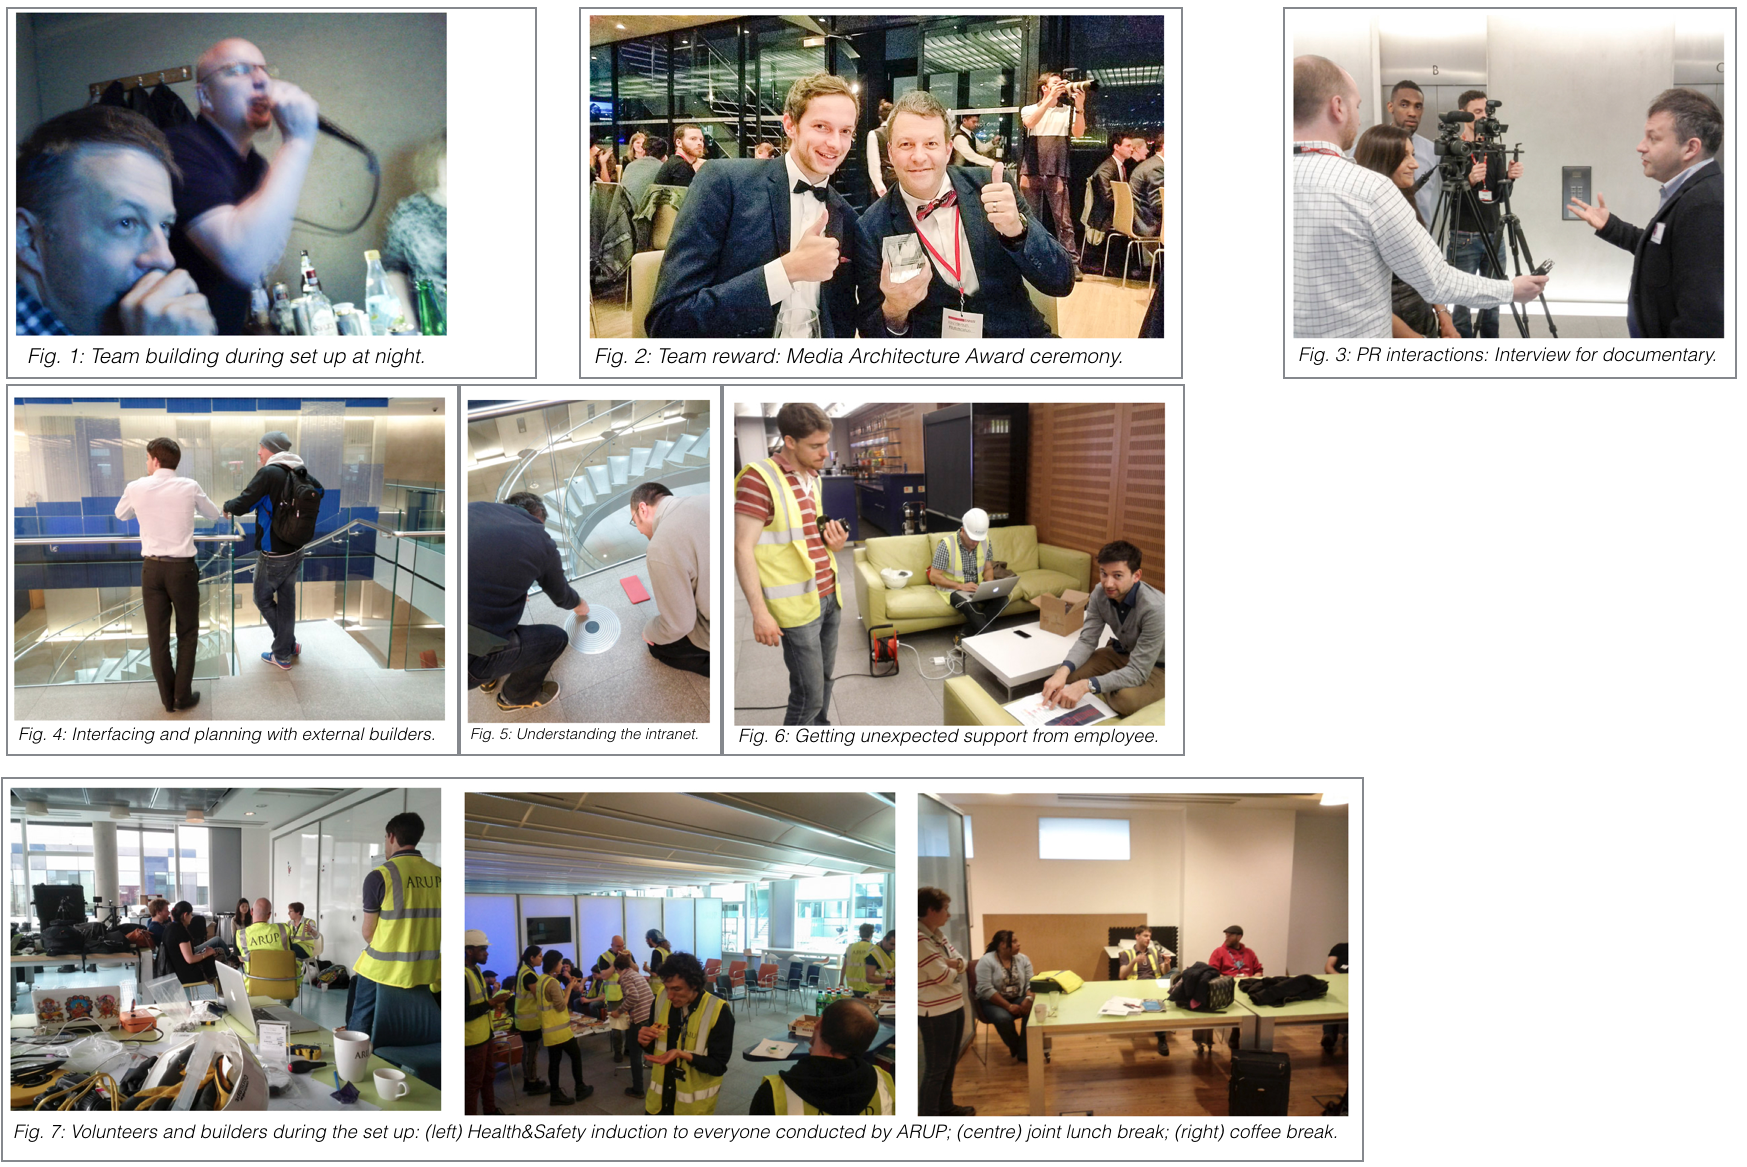
\includegraphics[width=\textwidth]{Illustrations/OnCollaboration.png}
\caption [On collaboration] {On collaboration}
\label{OnCollaboration}
\end{figure}



\subsection*{Managing expectations – the client relationship}

As a matter of fact the different parties involved in this project wanted to achieve the same goals (i.e. completion of the Sentiment Cocoon) their motivations however were different. For Arup it seemed to be the priority to showcase the Cocoon as a structure as well as a vision for better workplaces to their clients in order to demonstrate Arup’s ability to innovation and to support new designers through this competition.
For us as the designers and researchers it was preliminary important to materialise and implement our vision and the containing research knowledge. And of course to increase our professional network, by showing our skills. 
At the same time, managing expectations was a tricky venture throughout the project. For instance when initially proposing a 3D printer during the competition people actually expected what they considered a 3D printer. When we came up with a pallet-wrapping robot, they were rather disappointed of this creature that looked more like a vacuum cleaner. However, considering the fact that the robot quickly got a name (i.e. Einstein) seemed to be a sign of some kind of affection. In addition, calling the new surface a cling film structure made the whole process of wrapping Cocoon sounded a bit trivial. 
Another issue rose when we were calling the pallet-wrapping machine a robot. The health and safety department was particularly concerned about workplace safety. An autonomous machine in an office space would have been an uncontrollably risk. Only when we demonstrated that this machine is not acting like an industrial robot arm being able to cause severe damage we were able to convince the person in charge to sign off this fabrication process.
In a nutshell, the challenge for a successful client relationship is a careful management of expectations.

\section{Social implications}



\subsection{Mediated behaviours}

\subsection{Longitudinal Aspects and Sustainable Interactions}



From a long-term perspective, the rate of direct interactions with the cocoon dropped considerably after five weeks. 
A reason for this could be that many users now seemed to understand how the cocoon worked and might have become tired of it. 
The data sets suggest that this started after week five of the deployment.
In the following weeks, peaks could be identified at certain events, such as the Arup summer party on Tuesday, July 14th. 
In particular, the transition from the novelty effect to the levelling off phase is a highly relevant observation that needs further exploration.



\begin{figure}[!h] 
\centering
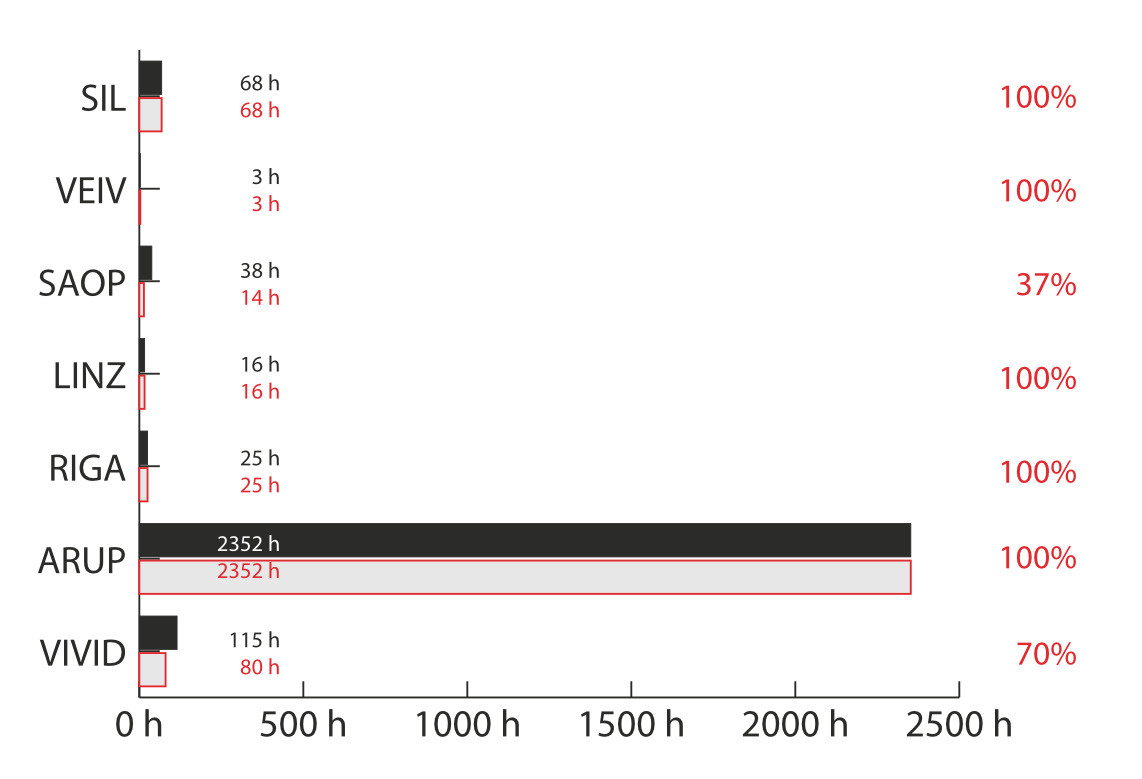
\includegraphics[width=\textwidth]{Illustrations/OverallStudyTimes.png}
\caption [Overall study times] {Overall study times.}
\label{OverallStudyTimes}
\end{figure}



\begin{figure}[!h] 
\centering
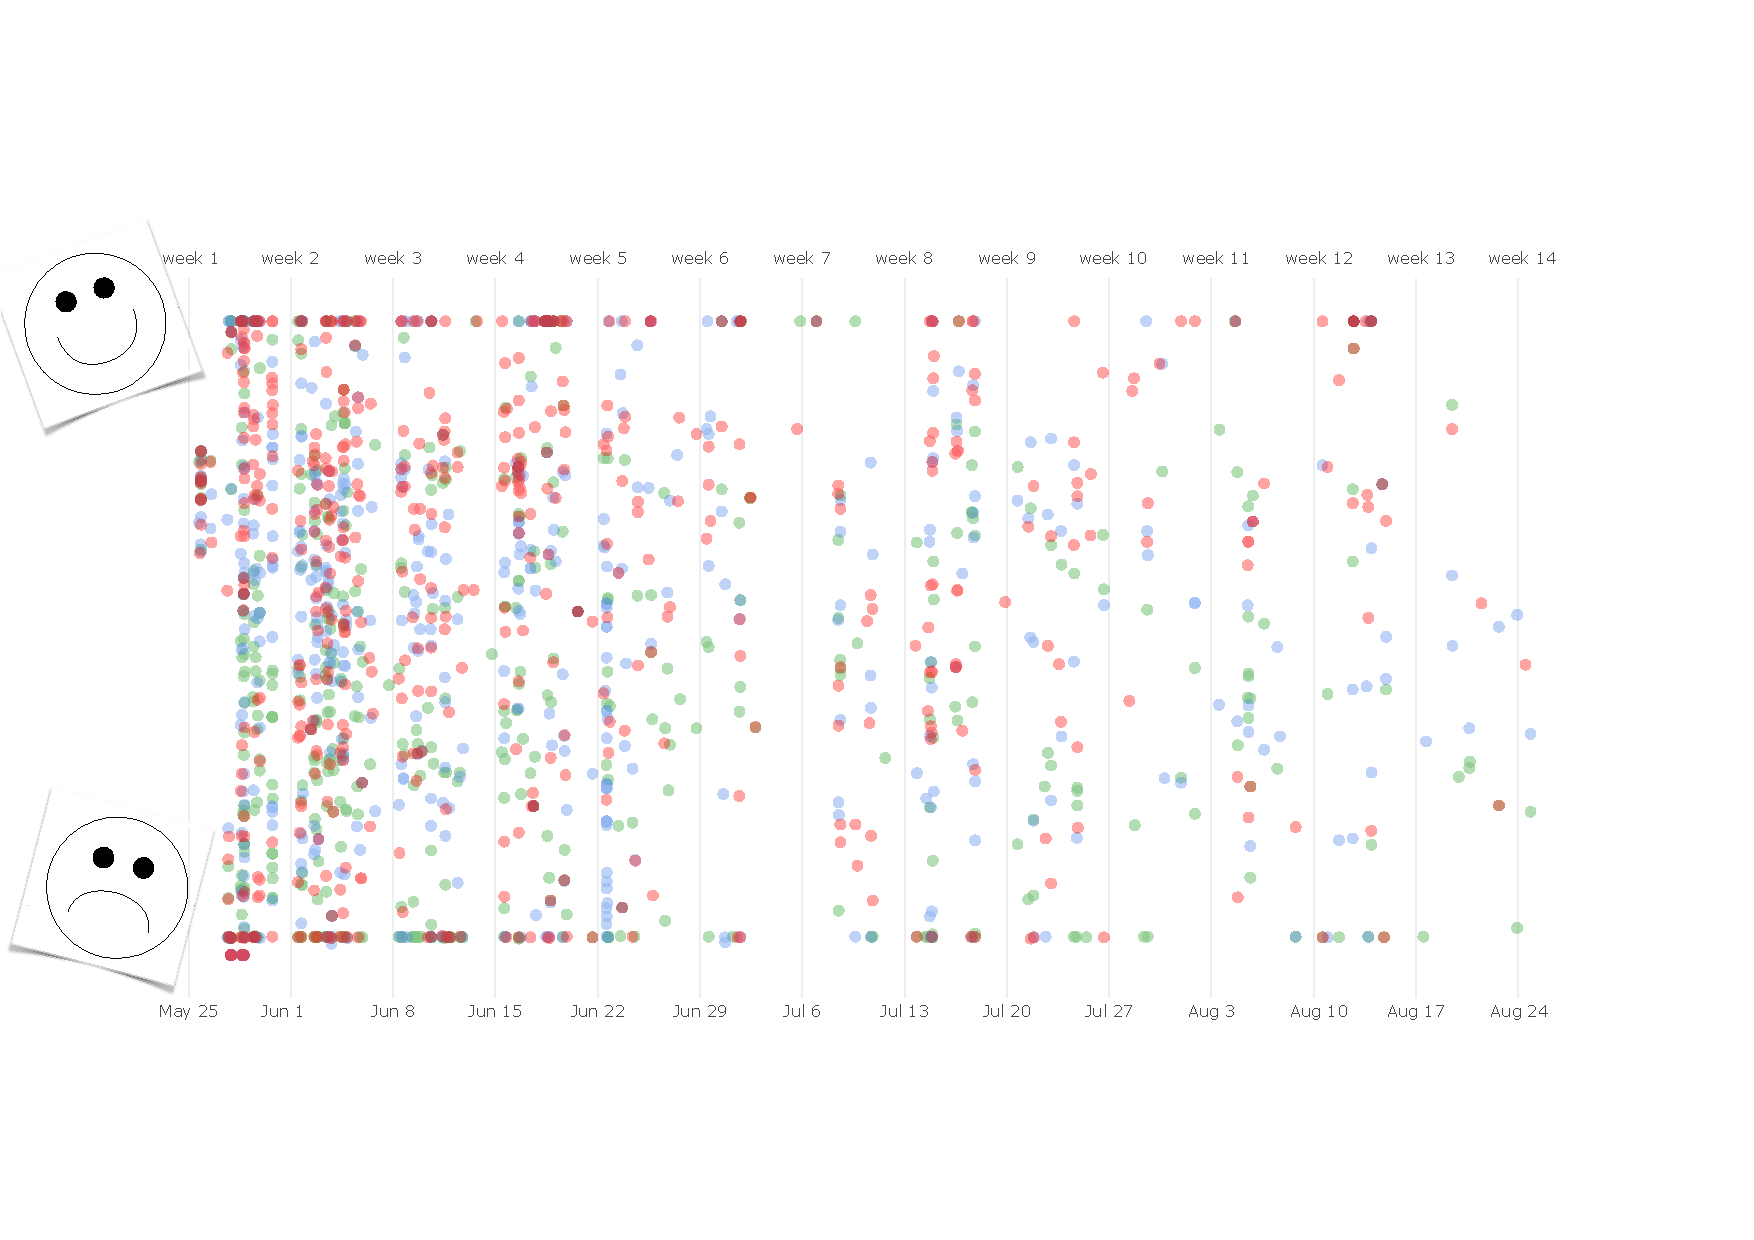
\includegraphics[width=\textwidth]{Illustrations/Sentiment-Analysis.pdf}
\caption [Longitudinal aspects] {Longitudinal data collected during the ARUP study: After week five one can clearly see that interactions with the sentiment interfaces slump.	}
\label{ARUPanalysis}
\end{figure}

\section{Spatial implications}

\subsection{Importance of space}

\subsection{Media architectural scale}

anthropometric scale versus people scale

\subsection{Ambient aspects of Media Architecture}

\subsection{Day versus Night aspects of Media Architecture}

"Despite this increasing urbanisation, we are not using our cities and towns to their fullest potential. Once shops and offices close for the evening, levels of activity in urban centres drop.
Night-time presents challenges to cities globally, be it for reasons of safety and fear, lack of destination or attraction."
Florence Lam, Arup Fellow Global Lighting Design Leader (Cities-Alive-Rethinking-Shades-of-Night.pdf)
\begin{figure}[!h] 
\centering
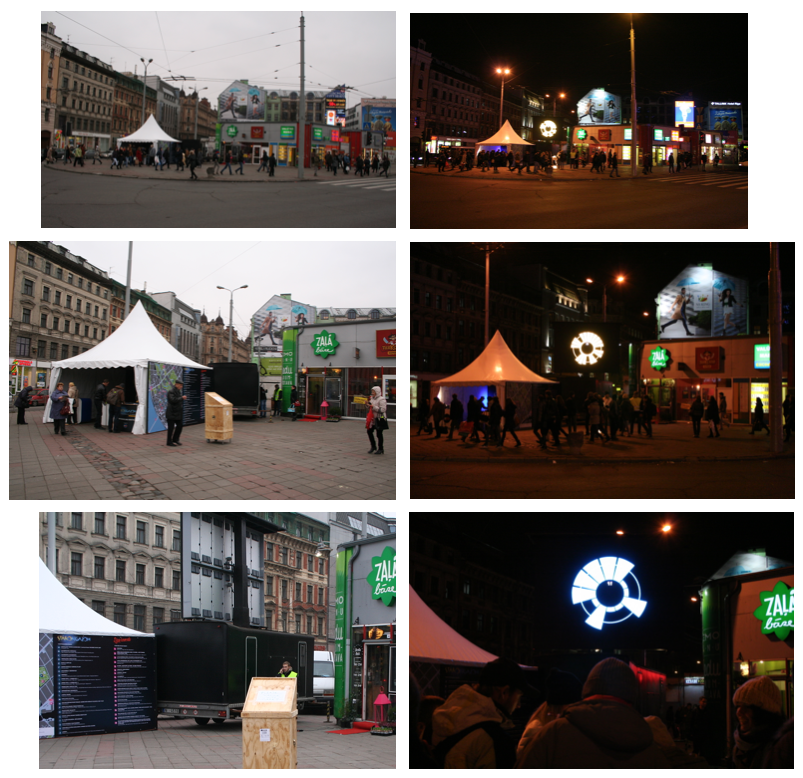
\includegraphics[width=\textwidth]{Illustrations/RIGA_day_night.png}
\caption [Day versus Night aspects of Media Architecture (RIGA)] {During the day the Urban Screen of our media installation was almost invisible within the urban context. During night time the circular appearance of our dynamic visualisation stood out amongst the mostly rectangular displays.}
\label{RIGAdaynight}
\end{figure}


\begin{figure}[!h] 
\centering
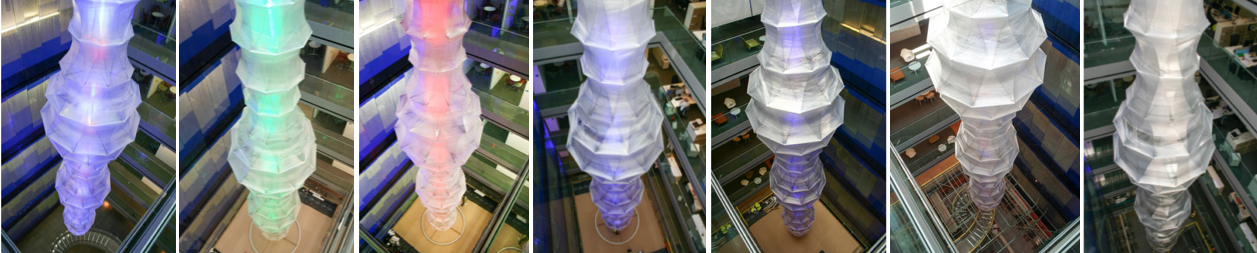
\includegraphics[width=\textwidth]{Illustrations/ARUP_daynight.png}
\caption [Day versus Night aspects of Media Architecture (ARUP)] {Natural daylight, flowing into the atrium from the skylights above, blends with the light emitted by the cocoon’s spine. 
This allows for rich interactions of varying forms of light, which are diffused through the skin of the cocoon. 
The translucency of the material fabricates an effect whereby the suspended cocoon generates a striking visual display of light that has been informed by the feelings of the building’s occupants.}
\label{ARUPdaynight}
\end{figure}

\begin{figure}[!h] 
\centering
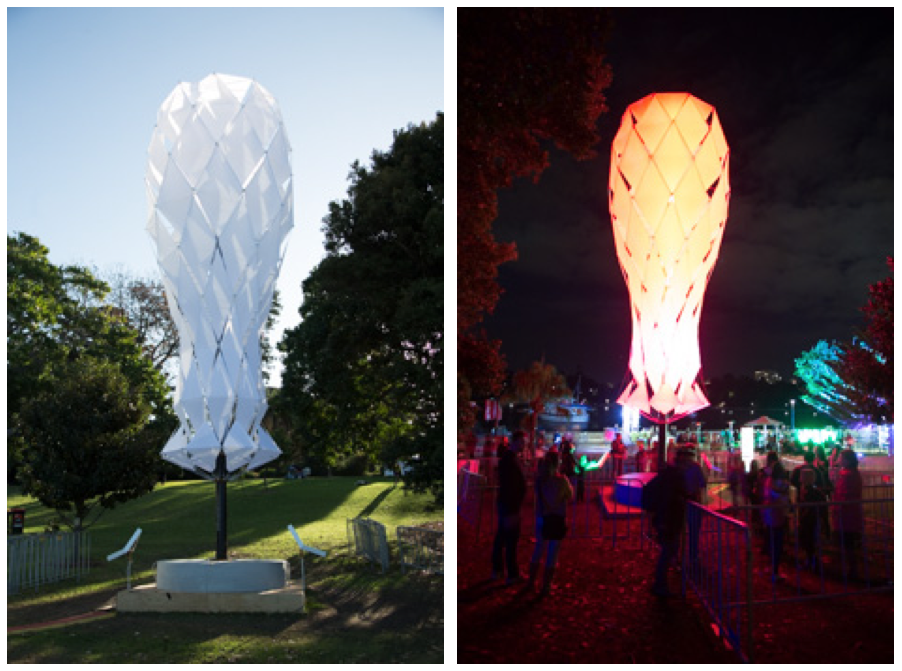
\includegraphics[width=\textwidth]{Illustrations/VIVID_daynight.png}
\caption [Day versus Night aspects of Media Architecture (VIVID)] {Aesthetically pleasing during day and night time: During day the construction and structural pattern of the cocoon become visible, the white sails and the interplay with natural daylight and the sun as well as the wind blowing through the sails creating a constantly changing appearance which develop their own intrinsic quality in contrast to the interactive colourful cocoon during night times. }
\label{RIGAdaynight}
\end{figure}






\chapter{Conclusion}
\label{chapterlabel7}

\section*{Chapter summary}

In this chapter I will introduce my research, which will lead to the main research question and the subsequent question that will assist to answer the main research question. Further an outline of the thesis will be conducted. This chapter then concludes with the overall contribution the reader can expect from reading this thesis.\newpage


\section{Future work}

\blindtext

\addcontentsline{toc}{chapter}{Appendices}




% The \appendix command resets the chapter counter, and changes the chapter numbering scheme to capital letters.
%\chapter{Appendices}
\appendix

\chapter{Media Mentions}
\label{appendixlabel1}
(stuff)

%\chapter{Another Appendix About Things}
%\label{appendixlabel2}
%(things)

\chapter{Colophon}
\label{appendixlabel3}
\textit{This is a description of the tools you used to make your thesis. It helps people make future documents, reminds you, and looks good.}

\textit{(example)} This document was set in the Times Roman typeface using \LaTeX\ and Bib\TeX , composed with a text editor. 
 % description of document, e.g. type faces, TeX used, TeXmaker, packages and things used for figures. Like a computational details section.
% e.g. http://tex.stackexchange.com/questions/63468/what-is-best-way-to-mention-that-a-document-has-been-typeset-with-tex#63503

% Side note:
%http://tex.stackexchange.com/questions/1319/showcase-of-beautiful-typography-done-in-tex-friends 


% This executes the index
\indexprologue{The index is meant to assist the reader to be reminded of key concepts }
\printindex


% You could separate these out into different files if you have
%  particularly large appendices.

% This line manually adds the Bibliography to the table of contents.
% The fact that \include is the last thing before this ensures that it
% is on a clear page, and adding it like this means that it doesn't
% get a chapter or appendix number.
\addcontentsline{toc}{chapter}{Bibliography}


% Actually generates your bibliography.
\bibliography{BibDesk_Moritz_130716}




% All done. \o/
\end{document}
